%=============================================================================
%  Disorder in Cavity-Coupled Jahn-Teller Active Molecules
%  Summer Internship Report -- Ann Lia Sam, NISER Bhubaneswar
%
%  Compile with:   pdflatex report.tex   (run twice for cross-references)
%  Figures live in ./figures/ ; no external bibliography tool is needed
%  (the reference list is a plain thebibliography environment).
%=============================================================================
\documentclass[12pt,a4paper]{article}

\usepackage[utf8]{inputenc}
\usepackage[T1]{fontenc}
\usepackage[a4paper,left=2.1cm,right=2.1cm,top=2.0cm,bottom=2.0cm]{geometry}
\usepackage{amsmath,amssymb,bm}
\usepackage{graphicx}
\usepackage{booktabs}
\usepackage{xcolor}
\usepackage{tikz}
\usetikzlibrary{arrows.meta,decorations.pathmorphing,positioning}
\usepackage[font=small,labelfont=bf]{caption}
\usepackage[section]{placeins}
\usepackage[colorlinks=true,linkcolor=blue!55!black,citecolor=blue!55!black,
            urlcolor=blue!55!black]{hyperref}

\graphicspath{{figures/}}
\raggedbottom
\linespread{0.96}

\setlength{\parskip}{0.5pt}
\renewcommand{\arraystretch}{1.1}
% compact float / caption spacing (keeps the report inside its page budget)
\setlength{\textfloatsep}{6pt plus 2pt minus 2pt}
\setlength{\intextsep}{6pt plus 2pt minus 2pt}
\setlength{\floatsep}{5pt plus 2pt minus 2pt}
\setlength{\abovecaptionskip}{3pt}
\setlength{\belowcaptionskip}{0pt}
% loosen default float placement limits -- this report is figure-dense
% (Sec. 7 alone has 6 case figures), and the defaults defer floats to
% specially-generated pages far from their referencing text.
\setcounter{topnumber}{4}
\setcounter{bottomnumber}{2}
\setcounter{totalnumber}{6}
\renewcommand{\topfraction}{0.90}
\renewcommand{\bottomfraction}{0.85}
\renewcommand{\textfraction}{0.05}
\renewcommand{\floatpagefraction}{0.65}

\newcommand{\JT}{\mathrm{JT}}
\newcommand{\Hc}{\hat H}
\newcommand{\ket}[1]{\left|#1\right\rangle}
\newcommand{\bra}[1]{\left\langle#1\right|}
\newcommand{\braket}[1]{\left\langle#1\right\rangle}
\newcommand{\PR}{\mathrm{PR}}
\newcommand{\hc}{\mathrm{H.c.}}

\title{\vspace{-1.2cm}\textbf{Disorder in Cavity-Coupled Jahn--Teller Active
Molecules}\\[0.25em]
\large From Single-Molecule Polaritons to Disorder-Averaged Collective Spectra}

\author{Ann Lia Sam\\[0.2em]
\normalsize National Institute of Science Education and Research (NISER), Bhubaneswar\\[0.4em]
\normalsize \textit{Under the guidance of} Prof.\ Krishna R.\ Nandipati and Prof.\ Athreya Shankar\\
\normalsize Indian Institute of Technology Madras}

\date{Summer Internship 2026}

\begin{document}

\thispagestyle{empty}
\begin{center}
\vspace*{0.3cm}
{\Large\bfseries Disorder in Cavity-Coupled Jahn--Teller Active\\
Molecules}\\[0.3em]
{\large From Single-Molecule Polaritons to Disorder-Averaged Collective Spectra}

\vspace{1.3em}
Summer Internship Report

\vspace{1em}
\textit{Under the guidance of}\\[0.2em]
\textbf{Prof.\ Krishna R.\ Nandipati}\\
Department of Chemistry\\
\textbf{Prof.\ Athreya Shankar}\\
Department of Physics

\vspace{2em}
\textit{Submitted by}\\[0.3em]
{\large\bfseries Ann Lia Sam}

\vspace{1em}
National Institute of Science Education and Research (NISER),\\
Bhubaneswar

\vspace{2.3em}

\includegraphics[height=2.7cm]{niser_logo.png}\hspace{2.3cm}%

\includegraphics[height=2.7cm]{iitm_logo.png}

\vspace{2.3em}
\textbf{Summer Internship 2026}
\end{center}

\newpage

\thispagestyle{empty}
\vspace*{3cm}
\begin{center}
{\LARGE\bfseries Acknowledgements}
\end{center}
\vspace{2em}
\noindent
I thank Prof.~Krishna R.~Nandipati and Prof.~Athreya Shankar (IIT Madras) for
their guidance throughout this internship, and for their valuable input during
every Thursday group meeting.
Special thanks to Suraj Kumar Pandit, PhD, and Abhinay Pandey, PhD, for
patiently clearing even my smallest doubts throughout this project.
I am also grateful to the entire lab for its warm and welcoming attitude
towards me during my time here.

\newpage

\thispagestyle{empty}
\vspace*{2cm}
\begin{center}
{\LARGE\bfseries Declaration}
\end{center}
\vspace{2em}
\noindent
I hereby declare that I have completed an internship under the guidance of
Prof.\ Krishna R.\ Nandipati (Department of Chemistry) and Prof.\ Athreya
Shankar (Department of Physics), Indian Institute of Technology Madras. I am
submitting a brief overview of my project to the National Institute of
Science Education and Research (NISER), Bhubaneswar.

\vspace{3em}
\begin{flushright}
Signature of the Student\\
Date:
\end{flushright}

\vspace{3em}
\noindent
The internship work reported in this document entitled \textbf{Disorder in
Cavity-Coupled Jahn--Teller Active Molecules} was carried out under our
supervision.

\vspace{3em}
\begin{flushright}
Signature of the Supervisor (Prof.\ Krishna R.\ Nandipati)\\
Date:
\end{flushright}

\vspace{2.5em}
\begin{flushright}
Signature of the Supervisor (Prof.\ Athreya Shankar)\\
Date:
\end{flushright}

\newpage

\thispagestyle{empty}

%=============================================================================
\section{Cavity--matter interaction}\label{sec:cavity}
%=============================================================================

A Fabry--P\'erot (FP) cavity is a pair of parallel mirrors separated by a
distance $L$ (Fig.~\ref{fig:cavity}). The mirrors quantise the electromagnetic
field inside into a discrete set of standing-wave modes of frequency
$\omega_c$ fixed by $L$, concentrating the vacuum field into a small mode
volume, which strongly enhances its interaction with any matter placed
inside.

When the light--matter coupling exceeds every loss rate in the problem (mirror
transmission, absorption, molecular linewidth), the system enters the
\emph{strong coupling} regime \cite{Ebbesen2016}: molecular excitation and
cavity photon can no longer be treated separately but hybridise into
\textbf{polaritons}, coherent superpositions of matter and light. The two
hybrid states - the \emph{lower} (LP) and \emph{upper} (UP) polariton -
are split by the \textbf{Rabi splitting} $\Omega$. Because they carry both
molecular and photonic character, strong coupling has become a route to
modifying photophysics and photochemistry without chemically altering the
molecules \cite{Ebbesen2016,Feist2018,Herrera2016}.

\begin{figure}[htbp]
\centering
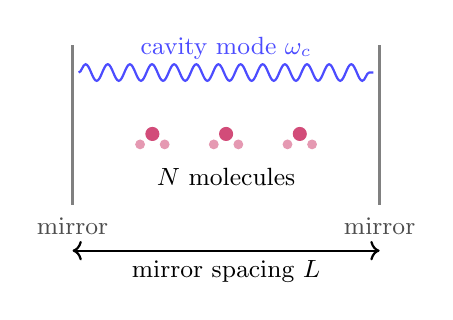
\begin{tikzpicture}[scale=0.78]
  \draw[very thick,gray] (0,0) -- (0,2.6);
  \draw[very thick,gray] (5.0,0) -- (5.0,2.6);
  \node[gray!60!black] at (0,-0.35) {\small mirror};
  \node[gray!60!black] at (5.0,-0.35) {\small mirror};
  \draw[blue!70,thick,decorate,decoration={snake,amplitude=3pt,segment length=8pt}]
       (0.1,2.15) -- (4.9,2.15);
  \node[blue!70] at (2.5,2.55) {\small cavity mode $\omega_c$};
  \foreach \x in {1.3,2.5,3.7}{
    \filldraw[purple!70] (\x,1.15) circle (3pt);
    \filldraw[purple!40] (\x-0.2,0.98) circle (2pt);
    \filldraw[purple!40] (\x+0.2,0.98) circle (2pt);
  }
  \node at (2.5,0.45) {\small $N$ molecules};
  \draw[<->,thick] (0,-0.75)--(5.0,-0.75);
  \node[below] at (2.5,-0.75) {\small mirror spacing $L$};
\end{tikzpicture}
\caption{$N$ molecules inside a Fabry--P\'erot cavity. The mirrors quantise
the field into discrete standing-wave modes of frequency $\omega_c$; in the
strong-coupling regime molecule and photon hybridise into polaritons.}
\label{fig:cavity}
\end{figure}
\FloatBarrier

The coupling in molecular polaritonics is also \emph{collective}: for $N$
identical molecules the bright (symmetric)
superposition of molecular excitations couples to the photon with a strength
enhanced by $\sqrt{N}$, so the Rabi splitting scales as $\Omega=2\sqrt{N}g$
with $g=\Omega/(2\sqrt N)$ the \emph{per-molecule} coupling. The remaining
$N-1$ orthogonal combinations carry no photon weight at all: they are the
\textbf{dark states}. This bright/dark separation is exact only for
\emph{identical} molecules, and its breakdown under disorder is the
subject of Secs.~\ref{sec:disorder}--\ref{sec:results}.

%=============================================================================
\section{Jahn--Teller active molecules and the $(E\times e)$ model}\label{sec:jt}
%=============================================================================

\begin{figure}[htbp]
\centering
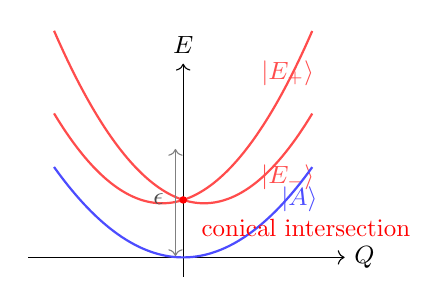
\begin{tikzpicture}[scale=0.82]
  \draw[->] (-2.4,0) -- (2.5,0) node[right]{\small $Q$};
  \draw[->] (0,-0.3) -- (0,3.0) node[above]{\small $E$};
  \draw[thick,red!70,domain=-2:2,samples=100,smooth]
    plot (\x,{0.9*(\x*\x*0.55 - 0.9) + 1.7 + 0.32*abs(\x)});
  \draw[thick,red!70,domain=-2:2,samples=100,smooth]
    plot (\x,{0.9*(\x*\x*0.55 - 0.9) + 1.7 - 0.32*abs(\x)});
  \node[red!70] at (1.62,2.85) {\small $\ket{E_+}$};
  \node[red!70] at (1.62,1.24) {\small $\ket{E_-}$};
  \draw[thick,blue!70,domain=-2:2,samples=100,smooth] plot (\x,{0.35*\x*\x});
  \node[blue!70] at (1.8,0.9) {\small $\ket{A}$};
  \draw[<->,gray] (-0.12,0.02) -- (-0.12,1.68);
  \node[gray!60!black,left] at (-0.15,0.9) {\small $\epsilon$};
  \filldraw[red] (0,0.89) circle (1.4pt);
  \node[red,anchor=west,scale=0.9] at (0.15,0.45) {conical intersection};
\end{tikzpicture}
\caption{Cut through the $(E\times e)$ potential energy surfaces along one
component of the degenerate mode coordinate $Q$: ground state $\ket{A}$
(blue) and the JT-split excited doublet (red), which touch at a conical
intersection. In the full two-dimensional $(Q_x,Q_y)$ space the lower excited
sheet is the ``Mexican hat''.}
\label{fig:mexicanhat}
\end{figure}
\FloatBarrier

The \textbf{Jahn--Teller (JT) theorem} \cite{JahnTeller1937} states that a
non-linear molecule in an orbitally degenerate electronic state is unstable:
it spontaneously distorts along a non-totally-symmetric coordinate so as to
lift the degeneracy. A standard example is the \textbf{$(E\times e)$
problem} \cite{LonguetHiggins1958,Bersuker2006,Koppel1984}, in which a doubly
degenerate electronic state $E$ (components $\ket{E_x},\ket{E_y}$) couples to
a doubly degenerate vibrational mode $e$ with coordinates $(Q_x,Q_y)$.

Molecules with an $n$-fold rotational axis $C_{n\ge3}$ possess such doubly
degenerate irreducible representations \cite{Nandipati2023}; planar aromatics
such as sym-triazine ($D_{3h}$) and benzene ($D_{6h}$) are standard examples
\cite{Whetten1986,Harris1989}, and the sym-triazine parameter set is used
throughout this work. Two properties of the $E$ subspace matter here: by
selection rules the two orthogonal polarisation directions of light
propagating along the $C_n$ axis couple the totally symmetric ground state
$\ket{A}$ to the corresponding $E_{x/y}$ component, and the vibronic coupling
between $\ket{E_x}$ and $\ket{E_y}$ mixes their electronic character.

It is convenient to work in the complex electronic basis
\begin{equation}
  \ket{E_\pm}=\frac{\ket{E_x}\pm i\ket{E_y}}{\sqrt2},
  \label{eq:Epm}
\end{equation}
in which the JT coupling has a transparent angular-momentum interpretation.
The adiabatic potential energy surfaces of the excited doublet form a
\emph{Mexican hat} with a \textbf{conical intersection} at the reference
geometry $Q_0$ (Fig.~\ref{fig:mexicanhat}); the nuclear motion around the
brim is a \emph{pseudorotation} that carries vibrational angular momentum,
which is what allows JT systems to exchange angular momentum with circularly
polarised light \cite{Nandipati2021}.

%=============================================================================
\section{Single molecule: cavity Jahn--Teller polaritons}\label{sec:1mol}
%=============================================================================

This section reproduces the model and the main spectroscopic result of
Nandipati and Vendrell \cite{Nandipati2023}.

\subsection{The cavity--Jahn--Teller Hamiltonian}

The molecule is placed inside the FP cavity with its $C_n$ axis along the
cavity axis $z$, so that the two normal-incidence cavity modes with
polarisations $(\bm e_x,\bm e_y)$ couple to the $E_x$ and $E_y$ excitations
respectively. The cavity-JT (CJT) Hamiltonian is
\begin{equation}
  \hat H=\hat H_{\JT}+\hat H_C+\hat H_{CM},
  \label{eq:Htot1}
\end{equation}
where $\hat H_{\JT}$ is the linear $(E\times e)$ JT Hamiltonian, $\hat H_C$
the cavity Hamiltonian, and $\hat H_{CM}$ the light--matter coupling. In the
electronic basis $\{\ket{E_+},\ket{A},\ket{E_-}\}$ the molecular JT
Hamiltonian reads \cite{Nandipati2023}
\begin{equation}
  \hat H_{\JT}=\sum_{r=+,-}\Big[\hbar\omega\,\hat b^\dagger_r\hat b_r
   +\epsilon\big(\ket{E_r}\bra{E_r}\big)\Big]
   +\frac{\kappa}{\sqrt2}\Big\{\big(\hat b^\dagger_++\hat b_-\big)
   \ket{E_-}\bra{E_+}+\hc\Big\},
  \label{eq:HJT}
\end{equation}
where $\omega$, $\epsilon$ and $\kappa$ are respectively the frequency of the
$e$ modes, the energy of the $E$ electronic states at the reference geometry
$Q_0$, and the linear JT coupling parameter. The vibrational ladder
operators are the circular combinations
\begin{equation}
  \hat b_\pm=\frac{\hat b_x\mp i\hat b_y}{\sqrt2},\qquad
  \hat b^\dagger_\pm=\frac{\hat b^\dagger_x\pm i\hat b^\dagger_y}{\sqrt2},
  \label{eq:bpm}
\end{equation}
with $\hat b_{x},\hat b_{y}$ the ladder operators of the real degenerate
modes $Q_x,Q_y$.

Written in this form, Eq.~\eqref{eq:HJT} makes explicit that the vibronic
coupling \emph{exchanges angular momentum} between the electronic subspace and
the vibrational pseudorotation. The vibrational angular momentum perpendicular
to the $(x,y)$ plane, and the electronic angular-momentum-like operator inside
the $E$ subspace, are
\begin{align}
  \hat L_z&=\hbar\big(\hat b^\dagger_+\hat b_+-\hat b^\dagger_-\hat b_-\big),
  &
  \hat S_z&=\hbar\big(\ket{E_+}\bra{E_+}-\ket{E_-}\bra{E_-}\big),
  \label{eq:LzSz}
\end{align}
the latter with eigenvalues $0,\pm\hbar$. The \emph{vibronic} angular momentum of the
molecular JT subsystem is then $\hat J_{\JT}=2\hat L_z+\hat S_z$, the factor
$2$ following from the $\pi$-radian (rather than $2\pi$) periodicity of the
pseudorotation \cite{LonguetHiggins1958}. One checks that
$[\hat H_{\JT},\hat J_{\JT}]=0$ - the symmetry of the linear $(E\times e)$
Hamiltonian responsible for the double degeneracy of the vibronic spectrum.

The cavity and the light--matter coupling are treated within the Condon
approximation of constant transition dipole and the rotating-wave
approximation:
\begin{align}
  \hat H_C&=\hbar\omega_c\big(\hat a^\dagger_+\hat a_++
             \hat a^\dagger_-\hat a_-\big),\nonumber\\
  \hat H_{CM}&=\frac{\Omega}{2}\big(\hat a^\dagger_+\ket{A}\bra{E_+}+
             \hat a^\dagger_-\ket{A}\bra{E_-}+\hc\big),
  \label{eq:HCM}
\end{align}
where $\hbar\omega_c$ is the cavity photon energy and $\Omega/2$ the
molecule--cavity coupling in energy units, so that at zero detuning the Rabi
splitting equals $\Omega$. As for the vibrations, circular cavity modes are
built from the linear polarisations,
$\hat a_\pm=(\hat a_x\mp i\hat a_y)/\sqrt2$ and
$\hat a^\dagger_\pm=(\hat a^\dagger_x\pm i\hat a^\dagger_y)/\sqrt2$
\cite{Crisp1991}; these carry photonic angular momentum $\pm\hbar$ and are
referred to as the cavity \emph{polarizations}. The
standing circular modes of a conventional-mirror cavity have a well-defined
angular momentum but no net helicity, since the helicities of the two
counter-propagating photon modes forming the standing wave cancel
\cite{Barnett2012}. The $z$ component of the photonic angular momentum is
\begin{equation}
  \hat l_z=\hbar\big(\hat a^\dagger_+\hat a_+-\hat a^\dagger_-\hat a_-\big).
  \label{eq:lz}
\end{equation}

\paragraph{Conservation law.} Defining the total vibronic--photonic angular
momentum
\begin{equation}
  \boxed{\ \hat J=2\hat L_z+\hat S_z+\hat l_z\ },
  \label{eq:Jtot1}
\end{equation}
one finds $[\hat H,\hat J]=0$ \cite{Nandipati2023}. The eigenstates of the
CJT Hamiltonian - the \textbf{JT polaritons} - are therefore labelled by
$j=2L+s+l$, with $L=n_+-n_-$ the pseudorotational quantum number
($n_\pm=0,1,\dots$ circular vibrational quanta), $s=0,\pm1$ labelling the
$\ket{A}$ and $\ket{E_\pm}$ electronic states, and $l=p_+-p_-$ where
$p_\pm=0,1$ are the circularly polarised photon occupations. States are doubly
degenerate with $j=\pm1$; absorbing a right-circularly polarised (RCP) photon
from the overall ground state reaches the $j=-1$ block, studied throughout.

\subsection{Result: the single-molecule polaritonic spectrum}

\begin{figure}[htbp]
\centering
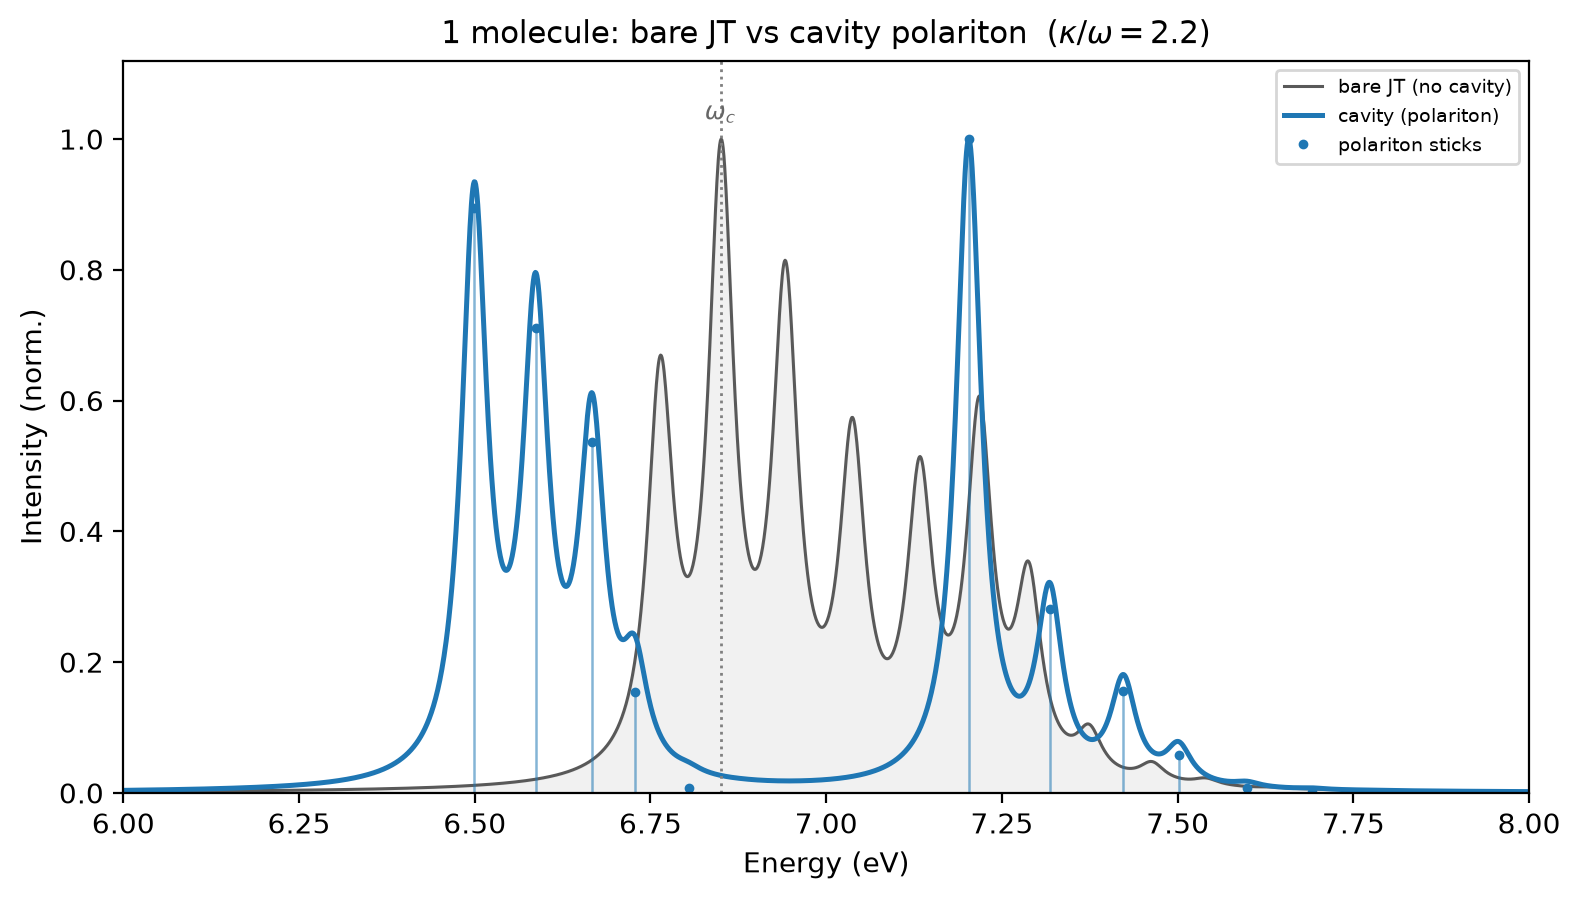
\includegraphics[width=0.62\textwidth]{fig_1mol_sticks.png}
\caption{Reproduction of the single-molecule cavity-JT polariton spectrum
\cite{Nandipati2023}. Grey: the bare $(E\times e)$ JT absorption spectrum of
sym-triazine (no cavity). Blue: the cavity (polaritonic) spectrum, with the
polaritonic stick spectrum underneath. Parameters $\epsilon=7$~eV,
$\omega=0.082$~eV, $\kappa/\omega=2.2$, $\omega_c=6.85$~eV,
$\Omega/2\omega_c=0.05$. The cavity is tuned to the brightest bare JT line;
the spectrum splits into LP and UP branches.}
\label{fig:1mol}
\end{figure}
\FloatBarrier

The absorption spectrum follows from diagonalising $\hat H$ in the
$(n_{\mathrm{ex}}=1,\ j=-1)$ block and taking the intensity of each eigenstate
as its overlap with the initial state (molecule in its vibronic ground state
plus one RCP photon). Figure~\ref{fig:1mol} shows the result for the
sym-triazine parameters $\epsilon=7$~eV, $\omega=0.082$~eV, $\kappa/\omega=2.2$
\cite{Whetten1986}, with $\omega_c=6.85$~eV resonant with the brightest bare
JT transition and $\Omega/2\omega_c=0.05$. Switching the cavity on
redistributes the bare JT oscillator strength (grey) into two well-separated
\textbf{LP} and \textbf{UP} branches of mixed vibronic--photonic peaks. What
matters for what follows is that at $N=1$ conservation
of $j$ together with $n_{\mathrm{ex}}=1$ restricts the molecule to only
\textbf{three vibronic sectors}, $v\in\{0,-1,-2\}$: the range is
\emph{bounded}.

%=============================================================================
\section{Collective vibronic cascade for $N$ molecules}\label{sec:2mol}
%=============================================================================

This section reproduces the model and the key observables of Pandit, Pandey,
Shankar and Nandipati \cite{Pandit2025}.

\subsection{Model}

We now consider $N$ JT active molecules coupled identically to the two
orthogonally polarised modes of the FP cavity. Each molecule $k$ has two
degenerate excited electronic levels well separated by an energy
$\epsilon=\hbar\omega_\epsilon$ from the ground state $\ket{A}$. In terms of
the linear combinations $\ket{E_\pm}=(\ket{E_x}\pm i\ket{E_y})/\sqrt2$ and
$\hat b^{(\dagger)}_\pm=(\hat b_x\pm i\hat b_y)^{(\dagger)}/\sqrt2$, the
Hamiltonian for molecule $k$ is ($\hbar=1$)
\begin{equation}
  \hat H_{m,k}=\sum_{r=+,-}\Big[\omega\,\hat b^\dagger_{r,k}\hat b_{r,k}
    +\omega_\epsilon\ket{E_r}_k\bra{E_r}_k\Big]
    +\kappa\Big[\big(\hat b^\dagger_{+,k}+\hat b_{-,k}\big)
    \ket{E_-}_k\bra{E_+}_k+\mathrm{h.c.}\Big],
  \label{eq:Hmk}
\end{equation}
the second line being the linear $(E\times e)$ JT interaction of strength
$\kappa$. Coupling the $\ket{A}\leftrightarrow\ket{E_\pm}$ transitions to the
two circularly polarised cavity modes within the rotating-wave approximation,
the total Hamiltonian is
\begin{equation}
  \hat H=\hat H_c+\sum_{k=1}^{N}\big(\hat H_{m,k}+\hat H_{m-c,k}\big),
  \label{eq:Htot2}
\end{equation}
with the free cavity Hamiltonian
$\hat H_c=\omega_c(\hat a^\dagger_+\hat a_++\hat a^\dagger_-\hat a_-)$ and
\begin{equation}
  \hat H_{m-c,k}=\frac{\Omega}{2\sqrt N}
    \big(\hat a^\dagger_+\ket{A}_k\bra{E_+}_k+
         \hat a^\dagger_-\ket{A}_k\bra{E_-}_k+\mathrm{h.c.}\big).
  \label{eq:Hmck}
\end{equation}
The normalisation by $\sqrt N$ compensates the collective enhancement of the
molecule--cavity coupling, so that the per-molecule strength
$\Omega/(2\sqrt N)=g$ is approximately independent of $N$; note that
Eq.~\eqref{eq:Hmck} reduces to Eq.~\eqref{eq:HCM} at $N=1$.

\subsection{Vibronic angular momentum, conserved quantities and sectors}

Defining the electronic and vibrational angular-momentum operators
$\hat S_{z,k}=\ket{E_+}_k\bra{E_+}_k-\ket{E_-}_k\bra{E_-}_k$ and
$\hat L_{z,k}=\hat b^\dagger_+\hat b_+-\hat b^\dagger_-\hat b_-$, the
molecular Hamiltonian commutes with the total \emph{vibronic} angular
momentum operator
\begin{equation}
  \hat V_k=2\hat L_{z,k}+\hat S_{z,k}.
  \label{eq:Vk}
\end{equation}
Its eigenstates therefore carry a well-defined vibronic quantum number $v$ and
group into \emph{sectors} of fixed $v$, in terms of which
\begin{equation}
  \hat H_{m,k}=\sum_{v}\sum_i \lambda^v_i\ket{\lambda^v_i}_k\bra{\lambda^v_i}_k,
  \label{eq:Hmk_diag}
\end{equation}
where $\lambda^v_i$ and $\ket{\lambda^v_i}$ are the $i$th eigenfrequency and
eigenstate in sector $v$. The ground manifold consists of trivial eigenstates
$\ket{A,n_+,n_-}$, populating only even $v$ since
$\hat V_k\ket{A,n_+,n_-}=2(n_+-n_-)\ket{A,n_+,n_-}$; the excited manifold
consists of non-trivial JT eigenstates which, because
$\hat S_z\ket{E_\pm}=(\pm1)\ket{E_\pm}$, populate only odd $v$.

The total Hamiltonian \eqref{eq:Htot2} conserves two quantum numbers: the
total number of electronic and photonic excitations,
\begin{equation}
  \hat N_{\mathrm{ex}}=\sum_{k=1}^{N}
    \big(\ket{E_+}_k\bra{E_+}_k+\ket{E_-}_k\bra{E_-}_k\big)
    +\hat a^\dagger_+\hat a_++\hat a^\dagger_-\hat a_-.
  \label{eq:Nex}
\end{equation}
Second, introducing the photonic angular momentum
$\hat P=\hat a^\dagger_+\hat a_+-\hat a^\dagger_-\hat a_-$, the total angular
momentum
\begin{equation}
  \hat J=\sum_{k=1}^{N}\hat V_k+\hat P .
  \label{eq:Jtot2}
\end{equation}
These follow respectively from the Jaynes--Cummings nature of the
cavity--molecule interaction and from the dipole selection rules, and let the
Hamiltonian be block-diagonalised into sectors of fixed
$(n_{\mathrm{ex}},j)$. All results below are obtained in the optically relevant
single-excitation sector $(n_{\mathrm{ex}}=1,\ j=-1)$.

\subsection{The collective vibronic cascade}

\begin{figure}[htbp]
\centering
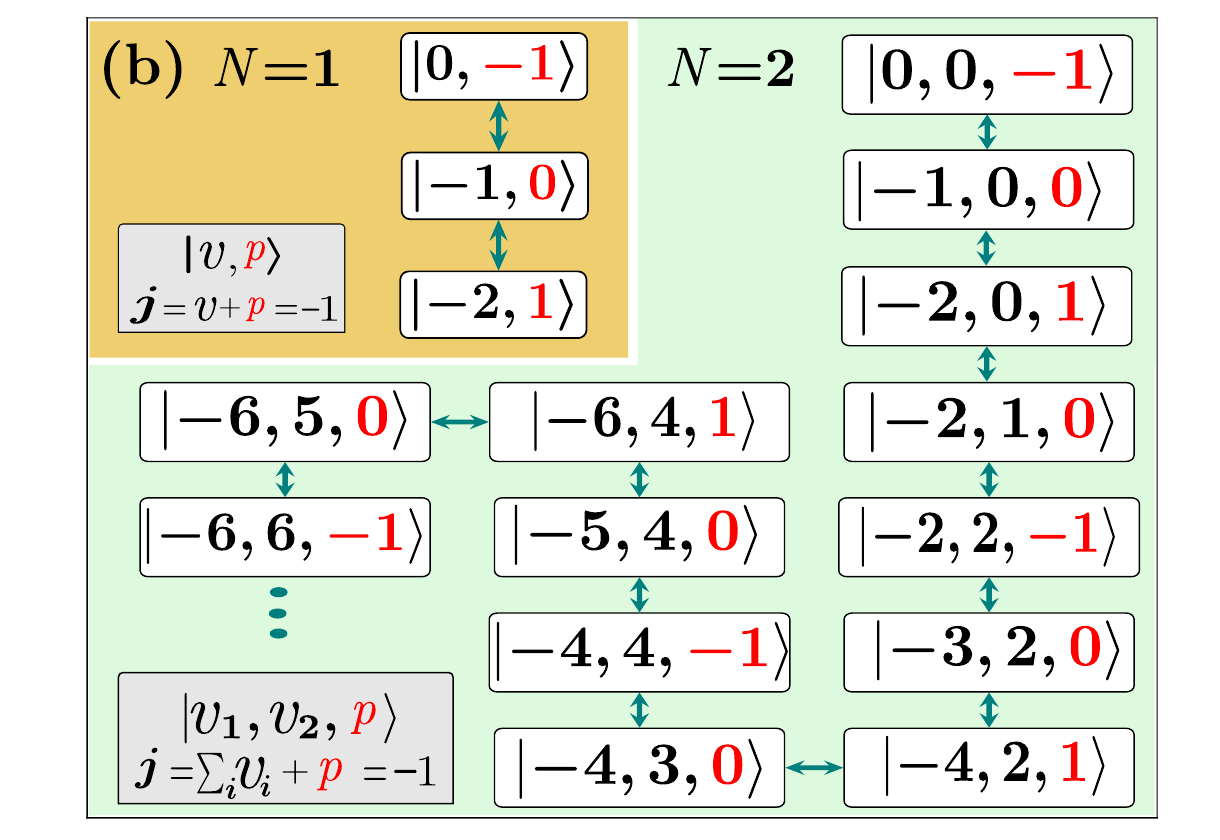
\includegraphics[width=0.62\textwidth]{fig2b_pandit2025.png}
\caption{Reproduction of Fig.~2(b) of Ref.~\cite{Pandit2025}: basis states
populated starting from all molecules in the vibronic ground state plus one
RCP photon, in the notation $\ket{v,p}$ ($N=1$) and $\ket{v_1,v_2,p}$ ($N=2$).
For $N=1$ the chain terminates after three sectors; for $N\ge2$ there is no
restriction on the individual $v_k$ and the ladder is unbounded - the
collective vibronic cascade.}
\label{fig:cascade}
\end{figure}
\FloatBarrier

For a \emph{single} molecule in the $(1,-1)$ sector the photon carries $p=-1$
(RCP) or $p=0$, and conservation of $j=-1$ forces $v\in\{0,-1,-2\}$ - the
bounded range behind the modest structure of Fig.~\ref{fig:1mol}.

For \emph{two or more} molecules this changes qualitatively. The conserved
quantity is the \emph{total} vibronic momentum $v=\sum_k v_k$, still
restricted to $\{0,-1,-2\}$, but the individual $v_k$ are now unconstrained:
one molecule can be driven to large positive $v_1$ provided the other
compensates with large negative $v_2$. Since the cavity photon is repeatedly
absorbed and re-emitted by different molecules, it \emph{mediates} the
transfer of angular momentum between them, generating the unbounded ladder of
Fig.~\ref{fig:cascade}: the \textbf{collective vibronic cascade}
\cite{Pandit2025}.

\subsection{Quantifying the cascade: sector population $P(v)$ and
participation ratio}

To quantify how far the cascade spreads, each polaritonic eigenstate is
decomposed over the single-molecule vibronic sectors. For $N=1$ these
eigenstates have the form
\begin{equation}
  \ket{\psi}=\sum_{v,i,p}C^v_{i,p}\ket{\lambda^v_i,p},
  \label{eq:psi1}
\end{equation}
where $p=0,\pm1$ indicates no cavity photon or one photon in the LCP/RCP
mode, so that the occupation of sector $v_0$ is simply
\begin{equation}
  P(v)=\sum_{i,p}\big|C^{v_0}_{i,p}\big|^2 .
  \label{eq:Pv1}
\end{equation}
For $N=2$ the permutation-symmetric eigenstates take the form
\begin{align}
  \ket{\psi}=&\sum_{v,i,p}C^v_{i,p}\ket{\lambda^v_i,\lambda^v_i,p}
   +\!\!\sum_{\substack{v,i,j,p\\ j>i}}\!\!C^v_{i,j,p}\tfrac{1}{\sqrt2}
   \big(\ket{\lambda^v_i,\lambda^v_j}+\ket{\lambda^v_j,\lambda^v_i}\big)\ket{p}
   \nonumber\\
  &+\!\!\sum_{\substack{v_1,v_2,i,j,p\\ v_2>v_1}}\!\!C^{v_1,v_2}_{i,j,p}
   \tfrac{1}{\sqrt2}\big(\ket{\lambda^{v_1}_i,\lambda^{v_2}_j}
   +\ket{\lambda^{v_2}_j,\lambda^{v_1}_i}\big)\ket{p},
  \label{eq:psi2}
\end{align}
and the probability of finding, say, molecule~1 in sector $v_0$ is
\begin{equation}
  P(v_0)=\sum_{i,p}\big|C^{v_0}_{i,p}\big|^2
   +\sum_{\substack{i,j,p\\ j>i}}\big|C^{v_0}_{i,j,p}\big|^2
   +\frac12\sum_{\substack{v,i,j,p\\ v<v_0}}\big|C^{v,v_0}_{i,j,p}\big|^2
   +\frac12\sum_{\substack{v,i,j,p\\ v>v_0}}\big|C^{v_0,v}_{i,j,p}\big|^2 .
  \label{eq:Pv2}
\end{equation}
The factor $1/2$ accounts for the symmetric structure of the two-molecule
state; by construction $\sum_v P(v)=1$. The spread over sectors is measured by
the \textbf{participation ratio}
\begin{equation}
  \PR=\frac{1}{\sum_v P^2(v)} .
  \label{eq:PR}
\end{equation}
$\PR=1$ means the state lives in a single sector; larger values mean it is
spread over many. For $N=1$ the bound $v\in\{0,-1,-2\}$ implies $\PR\le3$,
whereas for $N=2$ values up to $\PR\approx20$ occur. The \textbf{$P(v)$
heatmap} plots, for every \emph{bright} polaritonic eigenstate ($x$ axis,
energy ordered), the distribution $P(v)$ over sectors $v$ ($y$ axis).

\subsection{Results: two-molecule spectra and the clean $P(v)$ heatmap}

\begin{figure}[htbp]
\centering
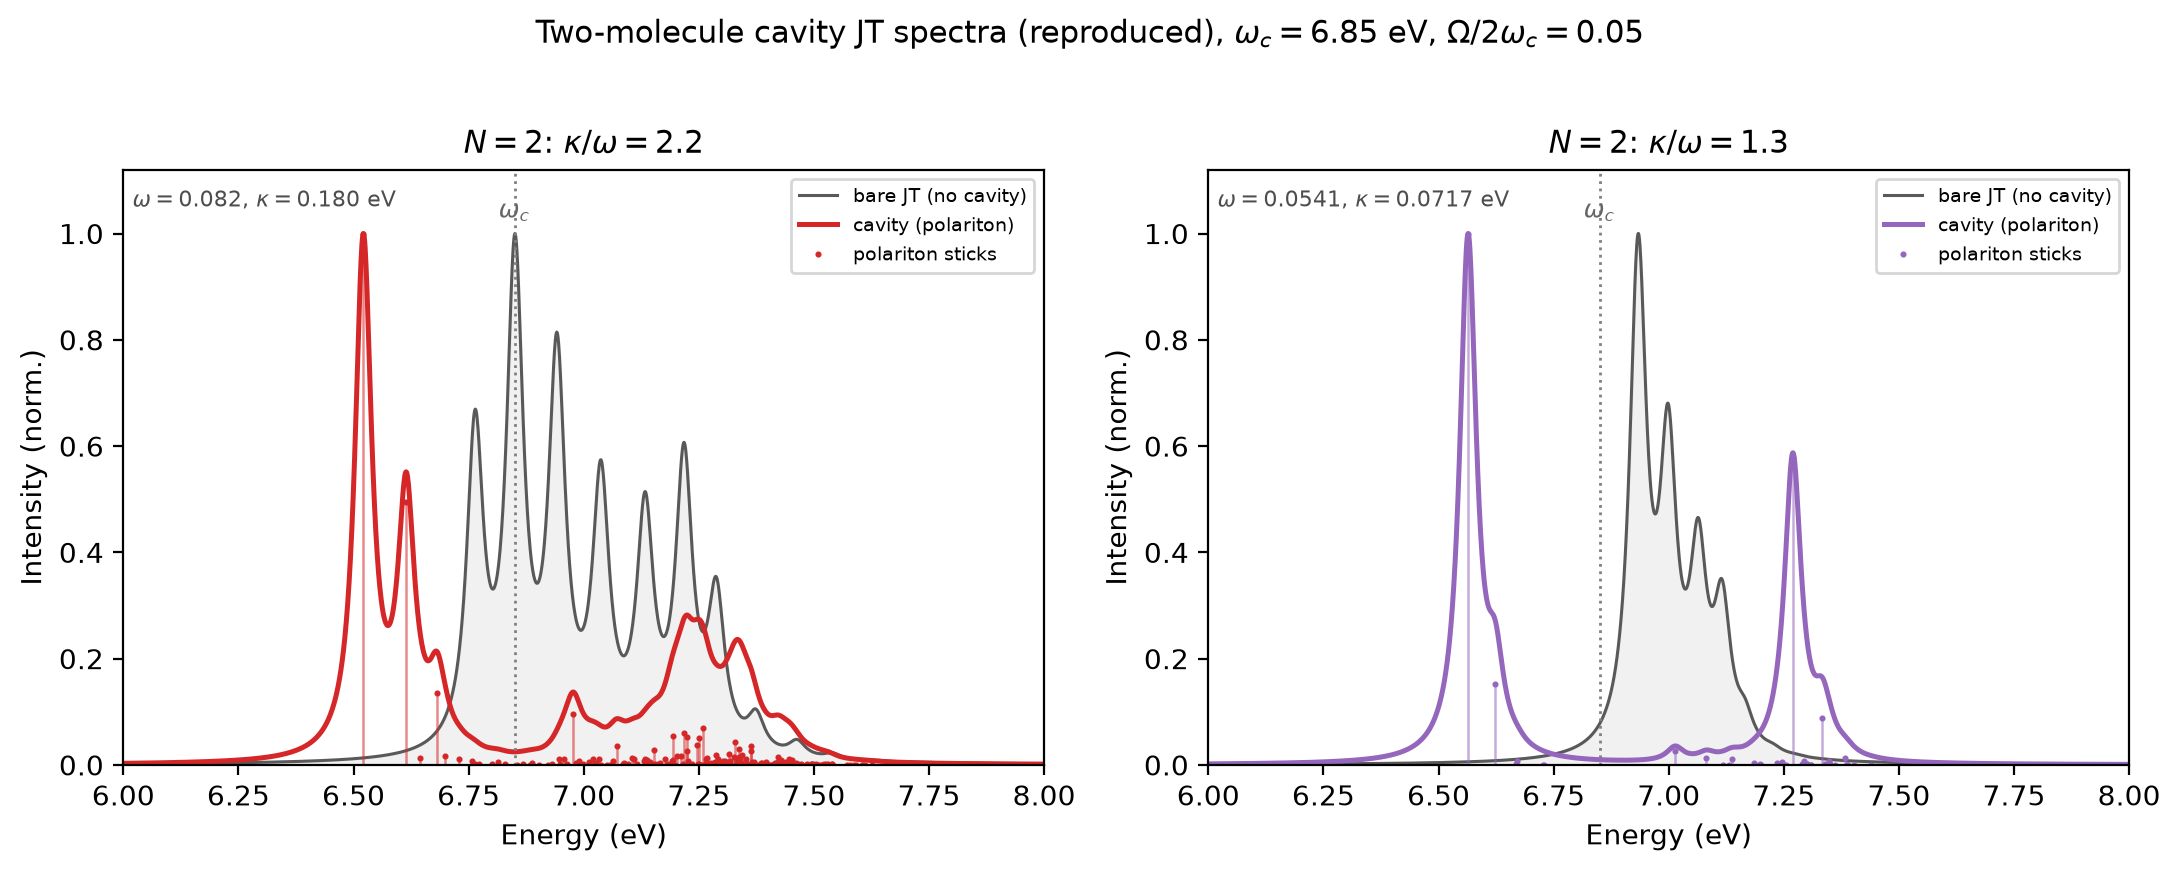
\includegraphics[width=0.80\textwidth]{fig_2mol_two_kappa.png}
\caption{Reproduction of the two-molecule cavity-JT polaritonic spectra
\cite{Pandit2025}. Grey: bare JT spectrum (no cavity). Coloured: $N=2$ cavity
polariton spectrum with the polaritonic stick spectrum (dots mark eigenstates
with intensity above a $10^{-2}$ relative tolerance). \textbf{Left:}
$\kappa/\omega=2.2$ ($\omega=0.082$~eV, $\kappa=0.180$~eV). \textbf{Right:}
$\kappa/\omega=1.3$ ($\omega=0.0541$~eV, $\kappa=0.0717$~eV). Both at
$\omega_c=6.85$~eV and $\Omega/2\omega_c=0.05$. The UP branch is visibly
broadened relative to the single-molecule case of Fig.~\ref{fig:1mol}.}
\label{fig:2mol}
\end{figure}
\FloatBarrier

\begin{figure}[htbp]
\centering
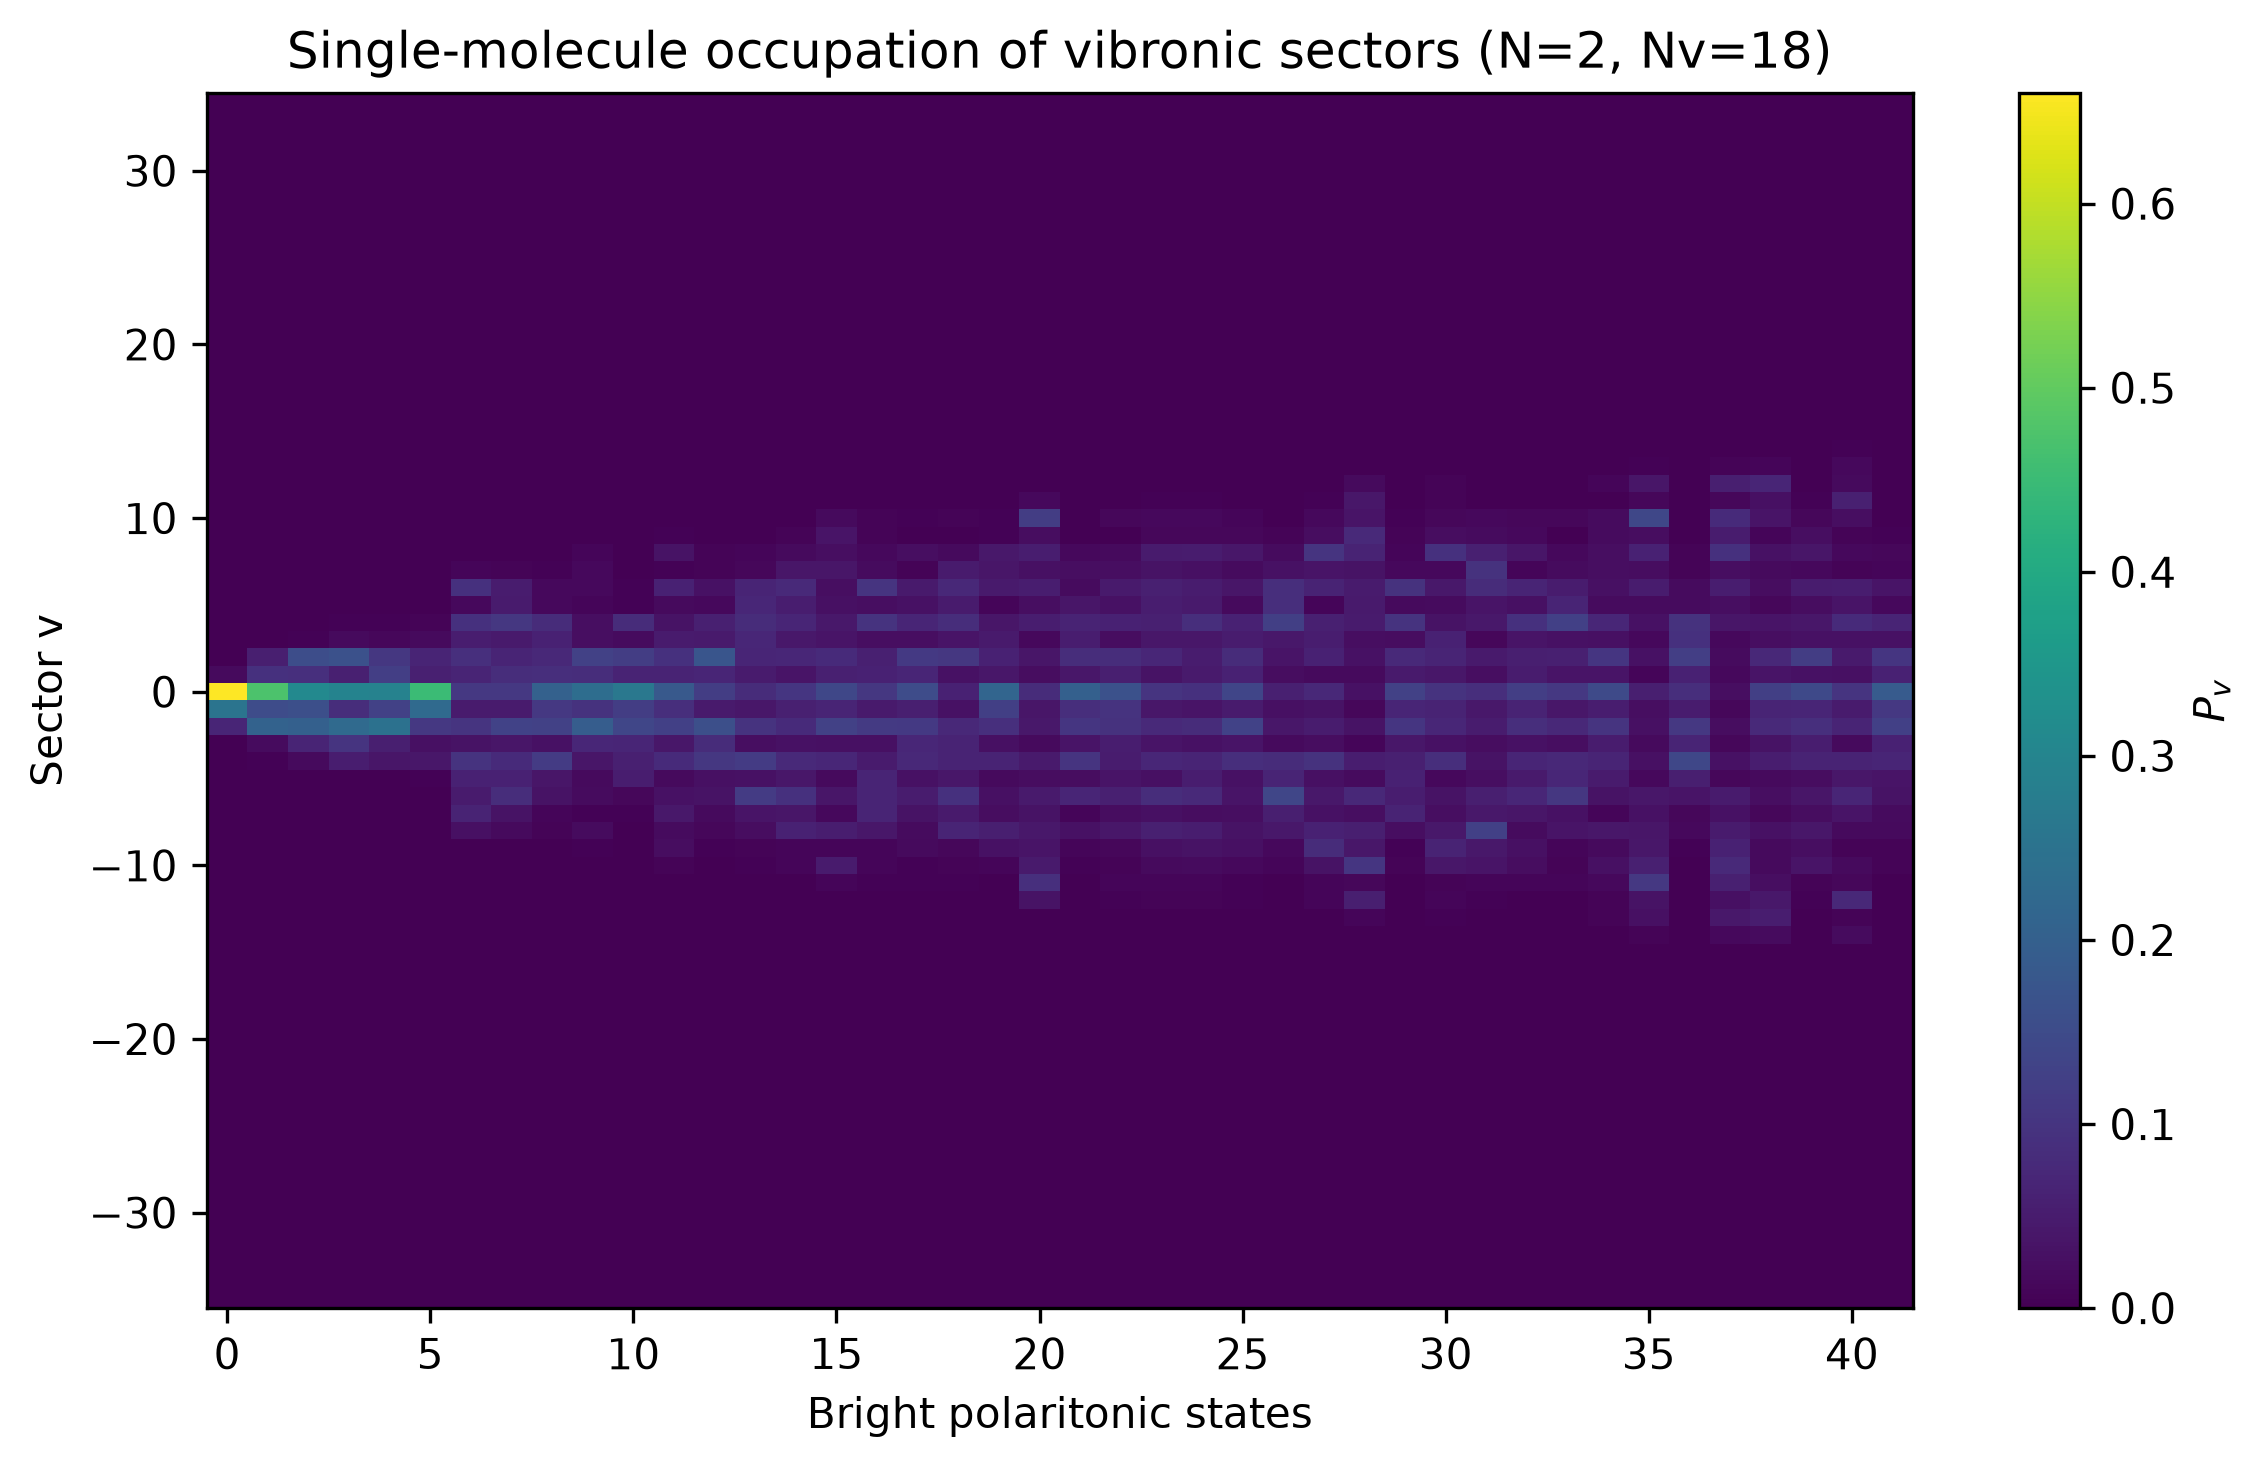
\includegraphics[width=0.48\textwidth]{fig_clean_heatmap.png}
\caption{Clean ($\sigma=0$) $N=2$ vibronic-sector heatmap, computed at
$\kappa/\omega=2.2$: the
single-molecule occupation probability $P(v)$ of each bright polaritonic
eigenstate. $x$: bright states in order of increasing energy; $y$: sector
$v$; colour: $P(v)$. Vibrational cutoff $N_v=18$. There are $42$ bright
eigenstates, $\PR_{\max}=19.9$, $\PR_{\mathrm{mean}}=12.7$, and sectors
$v\in[-14,13]$ are populated. This is the reference against which every
disordered case in Sec.~\ref{sec:results} is compared.}
\label{fig:cleanheatmap}
\end{figure}
\FloatBarrier

Figure~\ref{fig:2mol} shows the $N=2$ polaritonic spectra for two vibronic
coupling strengths. Compared with $N=1$ (Fig.~\ref{fig:1mol}), the LP branch
remains fairly well resolved but the UP branch broadens into many short stems
- a clear signature of the cascade, since a large number
of polaritonic states form that respond only weakly to cavity driving.
Figure~\ref{fig:cleanheatmap} makes the mechanism explicit: the bright states
spread over $v\in[-14,13]$ with $\PR$ reaching $\approx20$, versus the hard
bound $\PR\le3$ of the single molecule. This heatmap is the quantitative
baseline for the whole disorder study.

%=============================================================================
\section{Introducing disorder}\label{sec:disorder}
%=============================================================================

\subsection{Why disorder?}

Both models above assume $N$ \emph{identical} molecules. Real ensembles are
inhomogeneous: local environments, conformations and strain shift the
electronic transition energy from molecule to molecule. This static
\emph{energy disorder} is the standard explanation for inhomogeneous
linewidths, and it destroys the permutation symmetry underlying the
clean bright/dark separation of Sec.~\ref{sec:cavity}. The outlook of
Ref.~\cite{Pandit2025} names the inclusion of disorder in molecular energies
as the natural next step for the cavity-JT problem; that is the gap this work
addresses.

\subsection{The disordered Holstein--Tavis--Cummings model}

\begin{figure}[htbp]
\centering
\begin{minipage}[c]{0.32\textwidth}
  \centering
  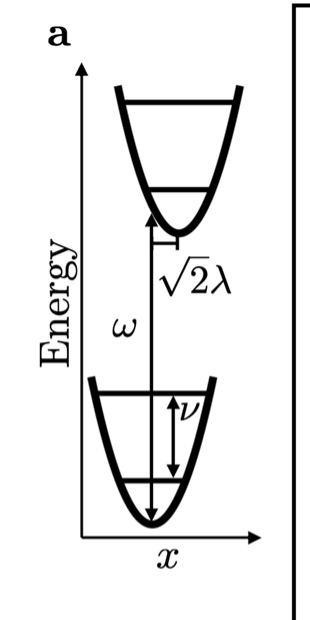
\includegraphics[width=0.78\linewidth]{fig_disorder_twolevel.png}
\end{minipage}\hfill
\begin{minipage}[c]{0.6\textwidth}
  \centering
  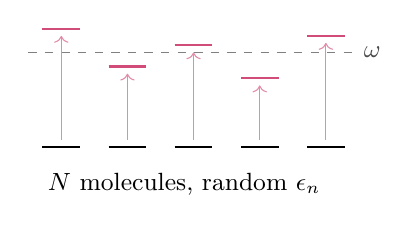
\begin{tikzpicture}[scale=0.60, every node/.style={font=\small}]
    \draw[dashed,gray] (-0.3,2) -- (6.6,2);
    \node[gray!60!black,anchor=west] at (6.6,2) {$\omega$};
    \foreach \x/\o in {0/0.5, 1.4/-0.3, 2.8/0.15, 4.2/-0.55, 5.6/0.35} {
      \draw[thick] (\x,0) -- (\x+0.8,0);
      \draw[thick,purple!70] (\x,2+\o) -- (\x+0.8,2+\o);
      \draw[->,purple!45,thin] (\x+0.4,0.15) -- (\x+0.4,{1.85+\o});
    }
    \node[below] at (3,-0.35) {$N$ molecules, random $\epsilon_n$};
  \end{tikzpicture}
\end{minipage}
\caption{\textbf{Left:} a two-level molecule on displaced harmonic surfaces
(vibrational spacing $\nu$, displacement $\sqrt2\lambda$) - the Holstein
model. \textbf{Right:} an ensemble of such molecules with random transition
energies $\omega+\epsilon_n$, the static energy disorder of
Ref.~\cite{Wellnitz2022}.}
\label{fig:twolevel}
\end{figure}
\FloatBarrier

The clearest framework for what disorder does to a cavity-coupled
molecular ensemble \emph{with vibrations} is the \textbf{disordered
Holstein--Tavis--Cummings (HTC)} model of Wellnitz, Pupillo and Schachenmayer
\cite{Wellnitz2022}: each molecule is a two-level system on a displaced
harmonic potential (Fig.~\ref{fig:twolevel}), with ($\hbar=1$)
\begin{equation}
  \hat H=\hat H_{\mathrm{TC}}+\hat H_{\mathrm{vib}}
        +\hat H_{\mathrm{H}}+\hat H_{\mathrm{dis}},
  \label{eq:HTC_total}
\end{equation}
with the Tavis--Cummings, vibrational, Holstein and disorder terms
\begin{align}
  \hat H_{\mathrm{TC}}&=\sum_{n=1}^{N}\Delta\,\hat\sigma^+_n\hat\sigma^-_n
     +g\sum_{n=1}^{N}\big(\hat a^\dagger\hat\sigma^-_n+\hat\sigma^+_n\hat a\big),
     \label{eq:HTC}\\
  \hat H_{\mathrm{vib}}&=\nu\sum_{n=1}^{N}\hat b^\dagger_n\hat b_n,
     \label{eq:Hvib}\\
  \hat H_{\mathrm{H}}&=\lambda\nu\sum_{n=1}^{N}
     \big(\hat b_n+\hat b^\dagger_n\big)\hat\sigma^+_n\hat\sigma^-_n,
     \label{eq:HH}\\
  \hat H_{\mathrm{dis}}&=\sum_n\epsilon_n\,\hat\sigma^+_n\hat\sigma^-_n .
     \label{eq:Hdis}
\end{align}
Here $\hat\sigma^\pm_n$ are the raising/lowering operators of the $n$th
molecule, $\Delta=\omega-\omega_C$ the detuning, $\lambda^2$ the dimensionless
Huang--Rhys factor, and $g\equiv g_c/\sqrt N$ the single-molecule coupling with
$g_c$ collective - the same $\sqrt N$ structure as Eq.~\eqref{eq:Hmck}. The
offsets $\epsilon_n$ have zero mean and variance $W^2$.

In the single-excitation subspace and in the clean limit,
$\hat H_{\mathrm{TC}}$ has two polariton eigenstates
$\ket{\pm}=\big(\hat a^\dagger/\sqrt2\pm\sum_n\hat\sigma^+_n/\sqrt{2N}\big)
\ket{0_{\mathrm{exc+ph}}}$ split by $2g_c$, plus $N-1$ degenerate dark states
of zero photon weight. Ref.~\cite{Wellnitz2022} quantifies two effects of
$\hat H_{\mathrm{dis}}$:
(i)~\textbf{Dark states brighten}: in perturbation theory the ``grey'' states
$\ket{d}$ acquire photon weight
$\sum_d|\braket{d|1_{\mathrm{ph}}}|^2\approx W^2/g_c^2$ (plus
$\approx\lambda^2\nu^2/2g_c^2$ from the Holstein term), so strictly invisible
states \textbf{appear in absorption}. (ii)~\textbf{Polaritons stay protected
while the coupling beats the disorder}: they are pushed outside the disorder
band by $\pm g_c$ and remain well-defined hybrid modes as long as
$W\lesssim g_c$, the model crossing over to the disorder-dominated regime
around $W\sim2g_c$.
The effect is \emph{non-monotonic}: disorder-enhanced excitation
transfer and vibrational entanglement \emph{peak} at $W\sim g_c$, rather than
growing without bound. Disorder is not simply detrimental.

\subsection{The arrowhead-matrix picture}

The reason for both effects is explained by the random
\textbf{arrowhead matrix} analysis of Dubail \emph{et al.} \cite{Dubail2021}:
in the single-excitation sector the disordered Tavis--Cummings Hamiltonian is
an $(N{+}1)\times(N{+}1)$ arrowhead matrix, with the random molecular energies
on the diagonal and the photon - the ``arrow tip'' - coupled to all of them
with strength $g_c/\sqrt N$. Two results are used here. First, the photon
weight of an eigenstate $\psi_a$,
\begin{equation}
  \mathrm{PW}_a=\big|\psi_{a,N+1}\big|^2\equiv
  \big|\braket{G,1|\psi_a}\big|^2,
  \label{eq:PW}
\end{equation}
is $O(1)$ for the two polaritons and $O(1/N)$ for each dark state (hence
$O(1)$ in total): the dark states collectively steal a finite share of the
photon. Second, the dark eigenvalues \emph{interlace} the bare molecular
energies, so the polaritons are the only outliers of the band; once the
disorder width exceeds the collective splitting they sink into the band and
lose their photon weight. Since absorption here starts from
$\ket{A,\dots,A;1_{\mathrm{ph}}}$, the intensity of an eigenstate \emph{is} its
photon weight: the spectra computed below are precisely the photon spectral
function $A(\omega)=\sum_a\mathrm{PW}_a\,\delta(\omega-\varepsilon_a)$ of
Ref.~\cite{Dubail2021}, and the $P(v)$ heatmap is its vibronic-sector
resolution.

%=============================================================================
\section{Disorder in the cavity-JT model: method and implementation}
\label{sec:method}
%=============================================================================

\subsection{How disorder enters}

Following Eq.~\eqref{eq:Hdis}, disorder is added to the cavity-JT model of
Sec.~\ref{sec:2mol} by making each molecule's excited-state energy random. In
the JT case each molecule has \emph{two} excited sublevels $\ket{E_\pm}$
which shift rigidly together, so the disorder term reads
\begin{equation}
  \hat H_{\mathrm{dis}}=\sum_{n}\epsilon_n\sum_{r=+,-}
    \hat\sigma^\dagger_{n,r}\hat\sigma_{n,r}
  =\sum_n\epsilon_n\big(\ket{E_+}\bra{E_+}_n+\ket{E_-}\bra{E_-}_n\big),
  \label{eq:Hdis_JT}
\end{equation}
with $\hat\sigma^\dagger_{n,r}=\ket{E_r}\bra{A}_n$ and
$\hat\sigma_{n,r}=\ket{A}\bra{E_r}_n$. Equivalently, and this is how it is
implemented, the transition energy of molecule $i$ in Eq.~\eqref{eq:Hmk} is drawn
independently from a Gaussian,
\begin{equation}
  \epsilon_i\sim\mathcal N\!\left(\epsilon,\,W^2\right),\qquad i=1,\dots,N,
  \qquad \epsilon=7.0~\mathrm{eV},
  \label{eq:gauss}
\end{equation}
so that $\delta_i=\epsilon_i-\epsilon$ has zero mean and variance $W^2$.
Throughout, $\sigma$ and $W$ denote the same disorder width.

\begin{table}[t]
\centering
\caption{Energy scales of the $N=2$ cavity-JT model with disorder. All values
in eV.}
\label{tab:scales}
\scriptsize
\begin{tabular}{@{}llll@{}}
\toprule
Quantity & Value & Quantity & Value\\
\midrule
vibrational quantum $\omega$ & $0.08196$ & JT coupling $\kappa$ ($\kappa/\omega=2.2$) & $0.180312$\\
cavity energy $\omega_c$ & $6.85$ & molecular energy $\epsilon$ & $7.0$\\
Rabi splitting $\Omega=2\sqrt N g$ ($\Omega/2\omega_c=0.05$) & $0.685$ & collective coupling $\sqrt N g=\Omega/2$ & $0.3425$\\
per-molecule coupling $g=\Omega/2\sqrt N$ & $0.2422$ & Lorentzian FWHM $\gamma$ & $0.025$\\
disorder width $W=\sigma$ & $0.48$ & ratios & $W/g=1.98$, $W/\Omega=0.70$\\
\bottomrule
\end{tabular}
\end{table}

\subsection{Choice of the disorder strength}

Table~\ref{tab:scales} collects the energy scales. The disorder width was
fixed at $W=0.48$~eV, i.e.
\begin{equation}
  \frac{W}{g}\approx2.0,\qquad \frac{W}{\sqrt N g}\approx1.4,
  \qquad \frac{W}{\Omega}\approx0.70 .
\end{equation}
In the language of Sec.~\ref{sec:disorder} this places the system just
\emph{below} the $W\sim2g_c$ crossover: nominally still strong coupling. A single strong value was chosen deliberately
rather than a weak/medium/strong sweep - at weak disorder every realization
simply reproduces the clean result, whereas at $W\approx2g$ the individual
realizations are physically distinct, which is what makes the case analysis
of Sec.~\ref{sec:results} informative. Figure~\ref{fig:gaussian} shows the
distribution.

\begin{figure}[htbp]
\centering
\begin{minipage}[t]{0.49\textwidth}
  \centering
  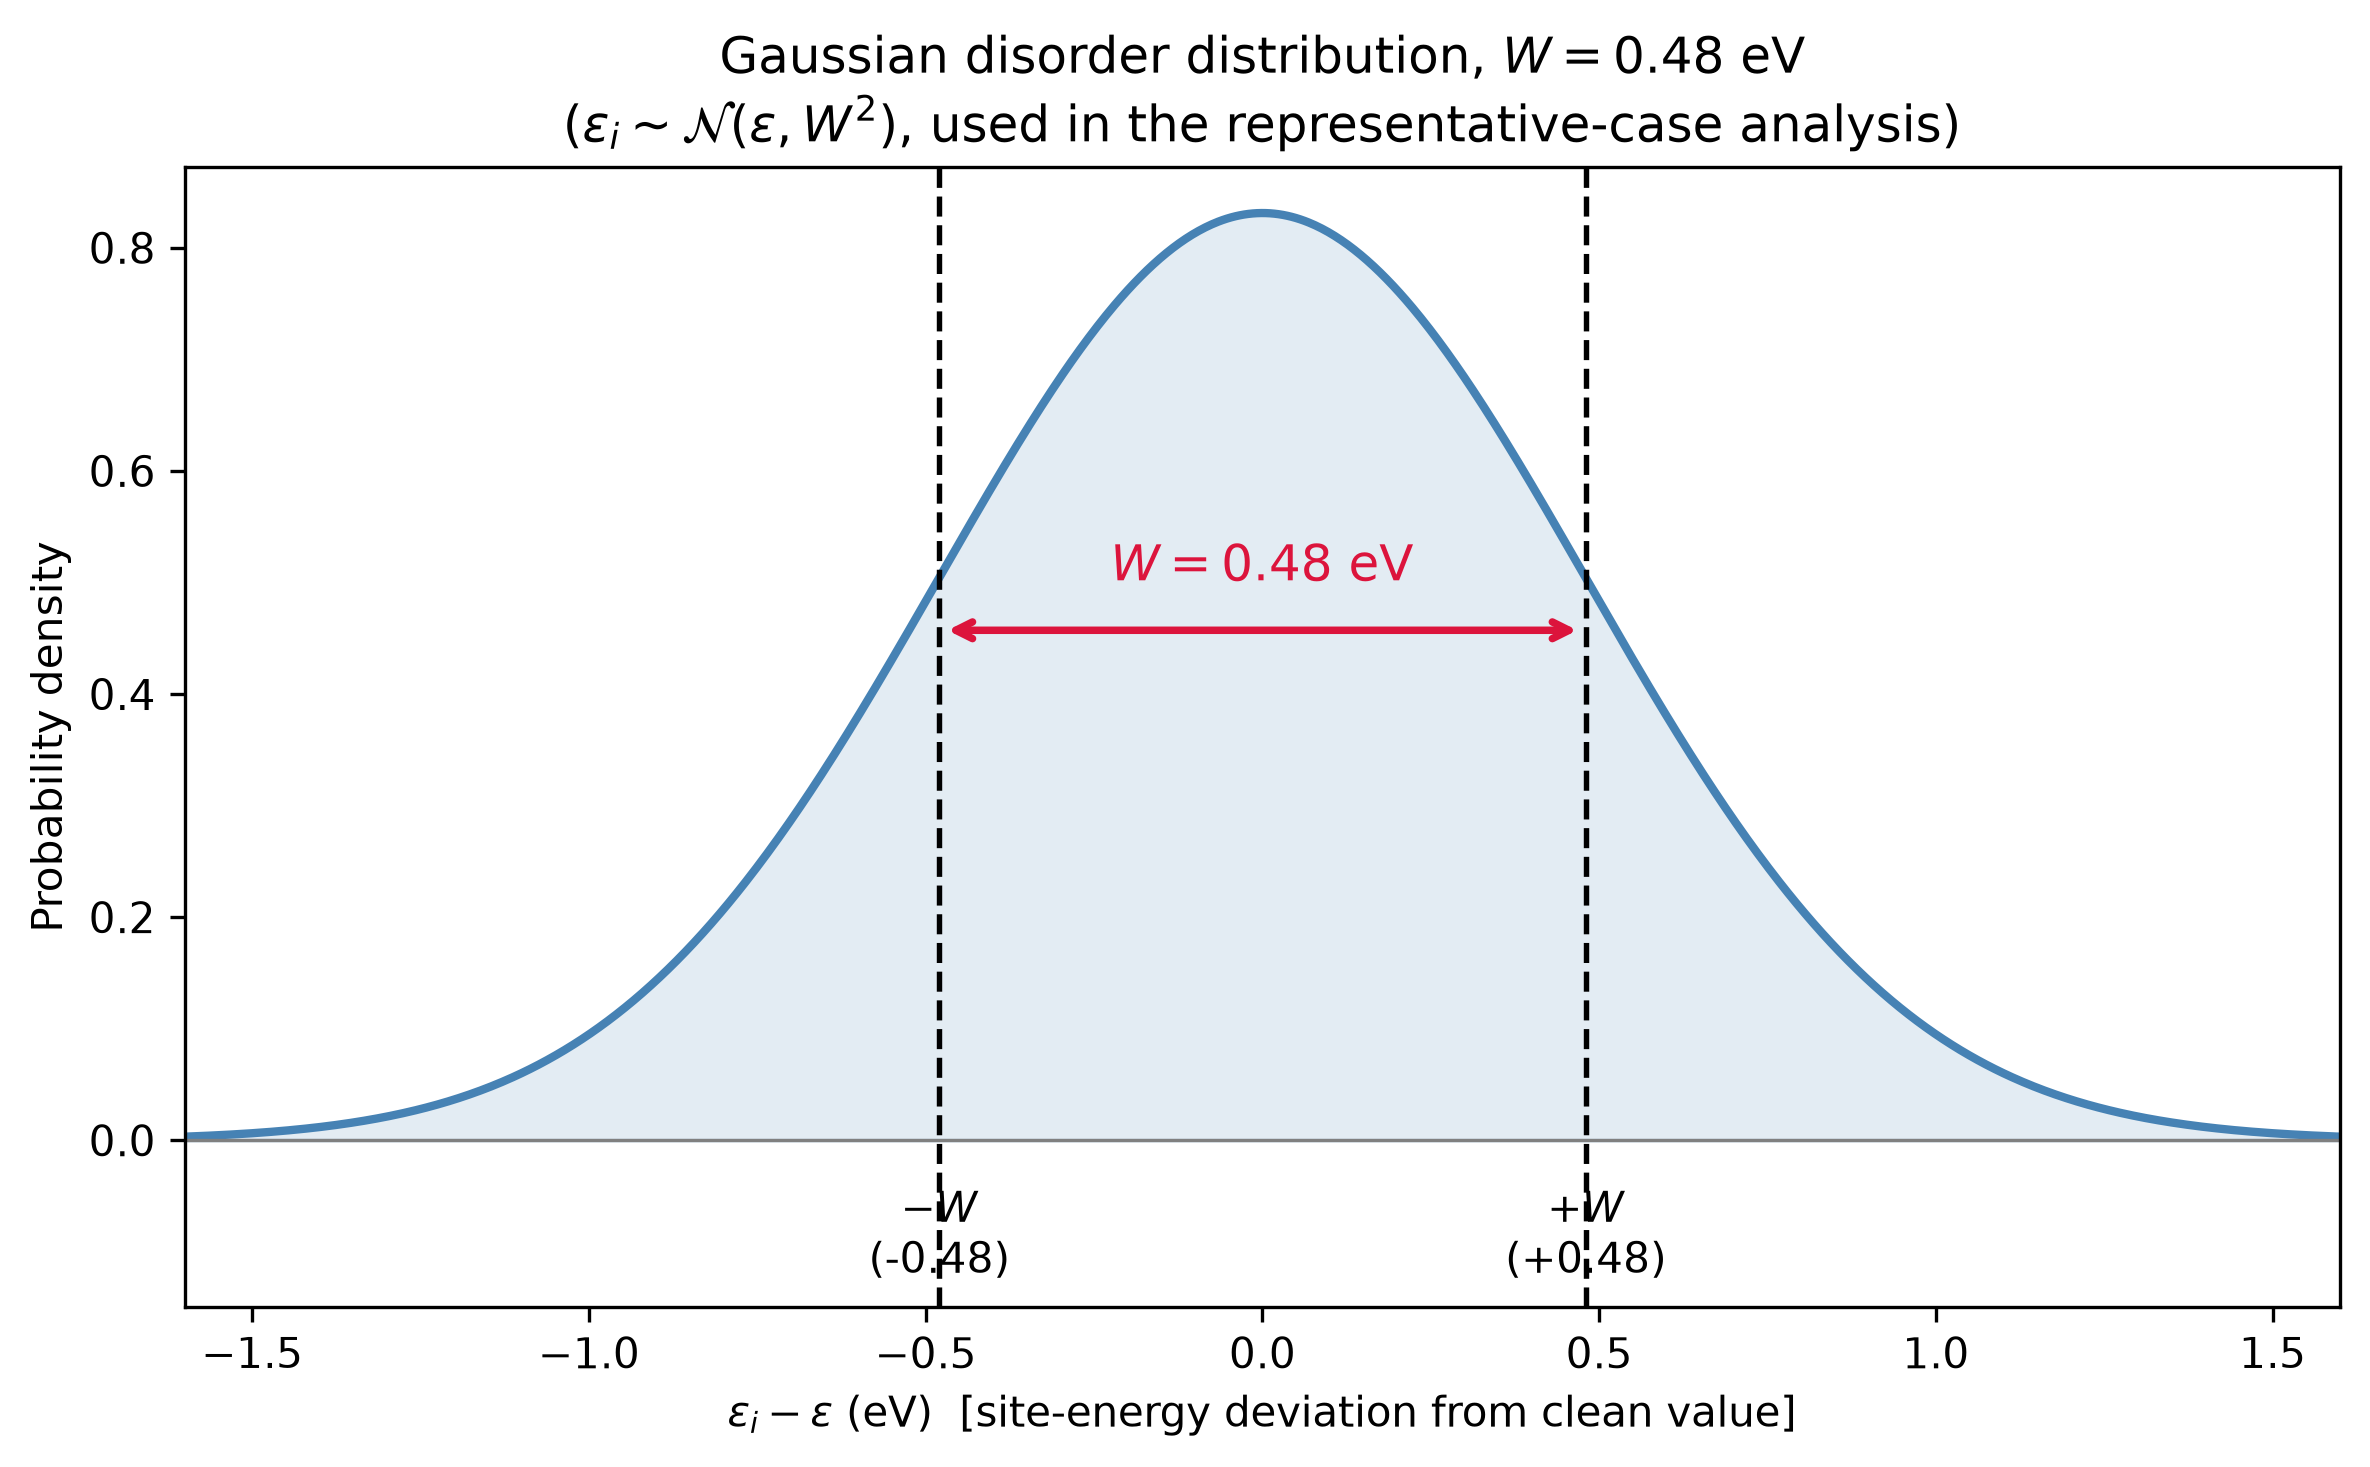
\includegraphics[width=0.98\linewidth]{fig_gaussian.png}
  \caption{Gaussian disorder distribution used throughout,
  $\epsilon_i\sim\mathcal N(\epsilon,W^2)$ with $W=0.48$~eV. Dashed lines
  mark $\pm W$. Absorption is averaged over $100$ realizations drawn from
  this distribution.}
  \label{fig:gaussian}
\end{minipage}\hfill
\begin{minipage}[t]{0.49\textwidth}
  \centering
  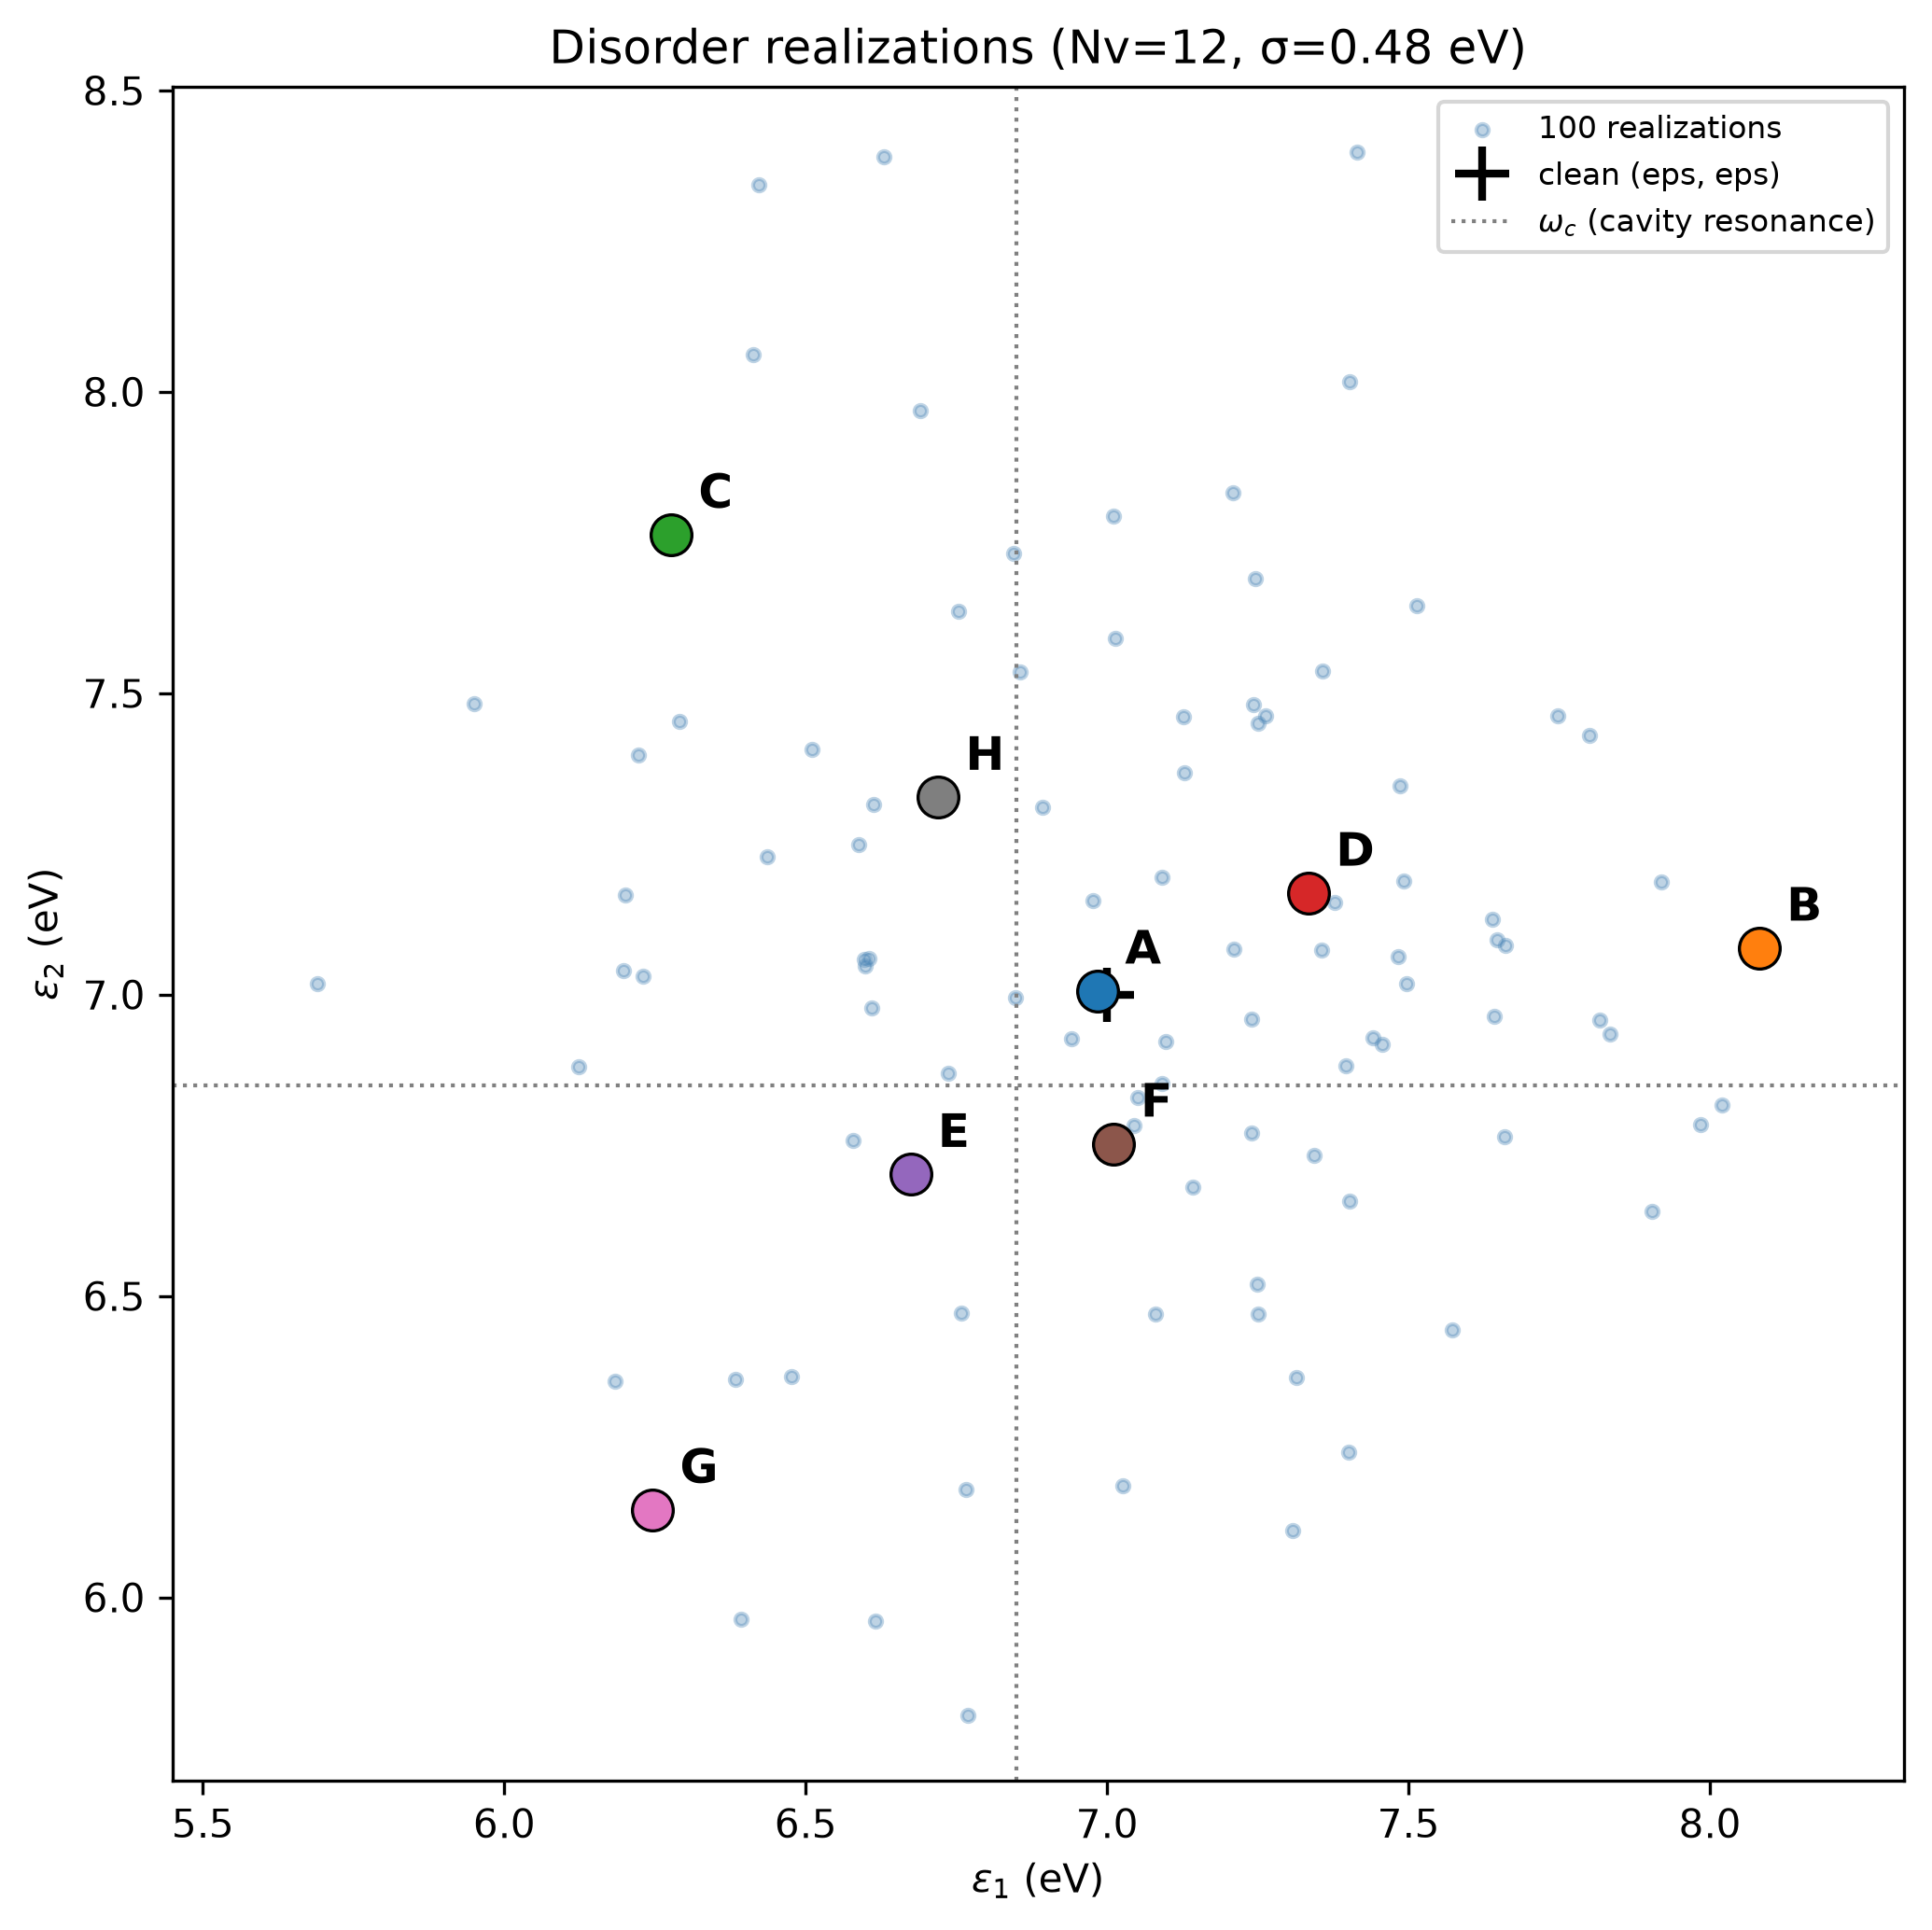
\includegraphics[width=0.78\linewidth]{fig_scatter.png}
  \caption{The $(\epsilon_1,\epsilon_2)$ cloud of $100$ disorder realizations
  at $W=0.48$~eV. Dotted lines mark $\omega_c$, the ``$+$'' marks the clean
  point $(\epsilon,\epsilon)$. Labelled points are the eight representative
  realizations A--H of Table~\ref{tab:cases}.}
  \label{fig:scatter}
\end{minipage}
\end{figure}
\FloatBarrier

\subsection{Numerical procedure}

For each disorder realization the following steps are carried out.

\begin{enumerate}\itemsep1pt
  \item \textbf{Basis construction.} A product basis state is the 8-tuple
  $(e_1,n_{+1},n_{-1},e_2,n_{+2},n_{-2},p_+,p_-)$, with $e_k\in\{A,E_+,E_-\}$,
  vibrational occupations $0\le n_{\pm k}<N_v$ and photon occupations
  $p_\pm\in\{0,1\}$. At $N_v=12$ the full product space has $746\,496$ states.
  \item \textbf{Symmetry filtering.} Only states with $n_{\mathrm{ex}}=1$
  [Eq.~\eqref{eq:Nex}] and $j=-1$ [Eq.~\eqref{eq:Jtot2}, evaluated as
  $j=2L_z+S_z+l_z$ with $L_z=(n_{+1}-n_{-1})+(n_{+2}-n_{-2})$,
  $l_z=p_+-p_-$] are kept, reducing the dimension to $6\,900$ - by a factor
  $108$ - which is what makes a converged $N_v=12$ calculation feasible.
  \item \textbf{Hamiltonian assembly.} The disorder-independent part of
  $\hat H$ (vibrational, cavity, JT and matter--cavity terms) is built
  \emph{once} per $N_v$; only the electronic diagonal, which carries
  $\epsilon_1,\epsilon_2$, is rebuilt per realization.
  \item \textbf{Diagonalization and intensities.} $\hat H$ is diagonalised;
  the absorption intensity of eigenstate $\ket{\psi_a}$ is
  $I_a=|\braket{i_0|\psi_a}|^2$ with
  $i_0=\ket{A,0,0;A,0,0;p_+{=}0,p_-{=}1}$, i.e.\ both molecules in the
  vibronic ground state plus one RCP photon. By Eq.~\eqref{eq:PW} this
  intensity is the photon weight of the eigenstate.
  \item \textbf{Broadening and averaging.} Each line is convolved with a
  Lorentzian of FWHM $\gamma$ and the result averaged over $M$ realizations,
  \begin{equation}
    A(E)=\frac{1}{M}\sum_{m=1}^{M}\sum_a I^{(m)}_a\,
    \frac{1}{\pi}\frac{\gamma/2}{\big(E-E^{(m)}_a\big)^2+(\gamma/2)^2},
    \label{eq:spec}
  \end{equation}
  on a grid of $2000$ points over $E\in[6,8]$~eV with $\gamma=0.025$~eV and
  $M=100$.
\end{enumerate}

For the $P(v)$ heatmaps a second, independent route is used, following the
Supplementary Material of Ref.~\cite{Pandit2025}: each molecule's JT
Hamiltonian \eqref{eq:Hmk} is diagonalised first to obtain the vibronic
eigenstates $\ket{\lambda^v_i}$ and their sector labels $v$; the two-molecule
plus cavity Hamiltonian is then built in that basis, restricted to
$(n_{\mathrm{ex}}=1,j=-1)$ and diagonalised, and $P(v)$, $\PR$ follow from
Eqs.~\eqref{eq:Pv2}--\eqref{eq:PR}. Since the JT eigenvectors are independent
of the transition energy (disorder shifts the excited eigenvalues rigidly), the
vibronic basis is computed once and reused for every realization. A state
counts as \textbf{bright} when its intensity exceeds $10^{-2}$ of the
brightest.

Because the sector-restricted dimension stays modest, everything here is
obtained by \emph{exact diagonalization}; Ref.~\cite{Pandit2025} complements
this with multi-configuration time-dependent Hartree (MCTDH) propagation
\cite{Vendrell2018} in order to reach $N=4$ and $N=8$, which is the route any
extension of this work to larger ensembles would have to take.

\subsection{Validation}

Because the disorder layers were added to an existing absorption pipeline, two
regression tests pin the results. The first checks that the
representative-realization analysis replays exactly the same random-number
stream as the disorder average - so a ``case'' really is one of the
realizations behind that average - and that the averaged spectrum is
unchanged by the addition. The second checks that the independent
vibronic-basis route used for the heatmaps reproduces the eigenvalues and
intensities of the direct product-basis route to $\sim10^{-9}$, and that
$\sum_vP(v)=1$ for every eigenstate. Case~A below, a near-zero-disorder draw,
is a further physical control: it must - and does - reproduce the clean
spectrum and heatmap.

%=============================================================================
\section{Results: representative disorder realizations}\label{sec:results}
%=============================================================================

\subsection{The $(\epsilon_1,\epsilon_2)$ cloud and the selection of cases}

A disorder-averaged spectrum such as Eq.~\eqref{eq:spec} hides the physics: it
superposes $100$ very different individual spectra. To recover the mechanism I
therefore analysed the cloud of drawn pairs $(\epsilon_1,\epsilon_2)$ directly
(Fig.~\ref{fig:scatter}) and selected \textbf{eight physically meaningful
realizations}, Cases A--H, each defined by a criterion on the \emph{actually
drawn} energies. Two natural coordinates organise the plane:
\begin{equation}
  s=\frac{\delta_1+\delta_2}{2}\quad\text{(common-mode shift)},\qquad
  \Delta=\epsilon_1-\epsilon_2\quad\text{(inter-molecular mismatch)},
\end{equation}
with $\delta_i=\epsilon_i-\epsilon$. These are orthogonal axes: $s$ moves both
molecules together relative to the photon and is compared with the collective
coupling $\sqrt N g$, whereas $\Delta$ breaks the permutation symmetry between
them and is compared with the per-molecule coupling $g$.

Note that $W$ is the Gaussian's standard deviation, not a hard bound
($\approx32\%$ of draws fall beyond $\pm1W$; here $38\%/35\%$ for
$\delta_1/\delta_2$). Three cases (B, C, G$^\dagger$) were selected by
\emph{maximizing} a detuning or mismatch and so land, by construction, at
$1.5$--$2.3\,W$ for at least one molecule - a locally stronger disorder
that drives them into the localized/decoupled regime of
Sec.~\ref{sec:results}, not a sampling inconsistency.

One point worth noting: a molecule is
\emph{cavity-resonant} when its brightest vibronic transition equals
$\omega_c$, which happens at $\epsilon_i\approx\epsilon=7.0$~eV and \emph{not}
at $\epsilon_i\approx\omega_c=6.85$~eV: $\omega_c$ was tuned to the clean
bright peak, which sits $\approx0.149$~eV below $\epsilon$ because of the JT
stabilisation. All criteria are therefore written in the signed detuning
$\delta_i$; case H is a deliberate exception targeting $\omega_c$ itself. The
cases are evaluated in order from a shared pool, so each claims a
\emph{distinct} realization.

\begin{table}[t]
\centering
\caption{The eight representative realizations selected from the $100$-draw
cloud at $W=0.48$~eV, with their selection criteria and outcomes.
$\delta_i=\epsilon_i-\epsilon$, $\Delta=\epsilon_1-\epsilon_2$,
$s=(\delta_1+\delta_2)/2$, $g=0.242$~eV. ``\#bright'' is the number of
polaritonic states with intensity above $10^{-2}$ of the maximum; the
$v$-range lists sectors with $P(v)>10^{-2}$ for at least one bright state.
The clean $\sigma=0$ reference is $42$ bright, $\PR_{\max}=19.9$,
$v\in[-14,13]$. $^\dagger$: $\ge\!1$ molecule has $|\delta_i|>W$ (tail draw; see text).}
\label{tab:cases}
\small
\setlength{\tabcolsep}{3.2pt}
\begin{tabular}{@{}clccccccc@{}}
\toprule
 & Criterion & $\epsilon_1$ & $\epsilon_2$ & $\Delta$ & $s/g$ &
 \#bright & $\PR_{\max}$ & $v$-range\\
\midrule
A & resonant baseline      & 6.984 & 7.006 & $0.02$ & $\phantom{-}0.0$ & 39 & 20.6 & $[-14,13]$\\
D & common blue detuning   & 7.334 & 7.169 & $0.17$ & $+1.0$ & 12 & 12.5 & $[-8,8]$\\
E & common red detuning    & 6.674 & 6.702 & $0.03$ & $-1.3$ & 104 & 22.4 & $[-15,14]$\\
F & single-mol.\ resonant  & 7.010 & 6.752 & $0.26\ (g)$ & $-0.5$ & 132 & 21.6 & $[-14,13]$\\
H & A--C line, interior    & 6.720 & 7.328 & $0.61\ (2.5g)$ & $\phantom{-}0.0$ & 46 & 16.2 & $[-10,9]$\\
C$^\dagger$ & opposite disorder (far)& 6.277 & 7.763 & $1.49\ (6g)$ & $\phantom{-}0.0$ & 14 & 8.5 & $[-10,10]$\\
B$^\dagger$ & large mismatch (same side) & 8.082 & 7.078 & $1.00\ (4g)$ & $+2.4$ & 11 & 3.8 & $[-8,8]$\\
G$^\dagger$ & bare-molecule limit    & 6.246 & 6.146 & $0.10$ & $-3.3$ & \phantom{0}8 & 4.5 & $[-4,3]$\\
\bottomrule
\end{tabular}
\end{table}

Table~\ref{tab:cases} lists the cases in the order discussed below, a physical
walk through the disorder plane rather than an alphabetical one: from the
resonant baseline A, moving the pair together (D, E), then breaking the
symmetry between the molecules by increasing amounts (F, H, C, B), and finally
decoupling both from the cavity (G).

\subsection{Case A - resonant baseline (effectively no disorder)}

\begin{figure}[htbp]
\centering
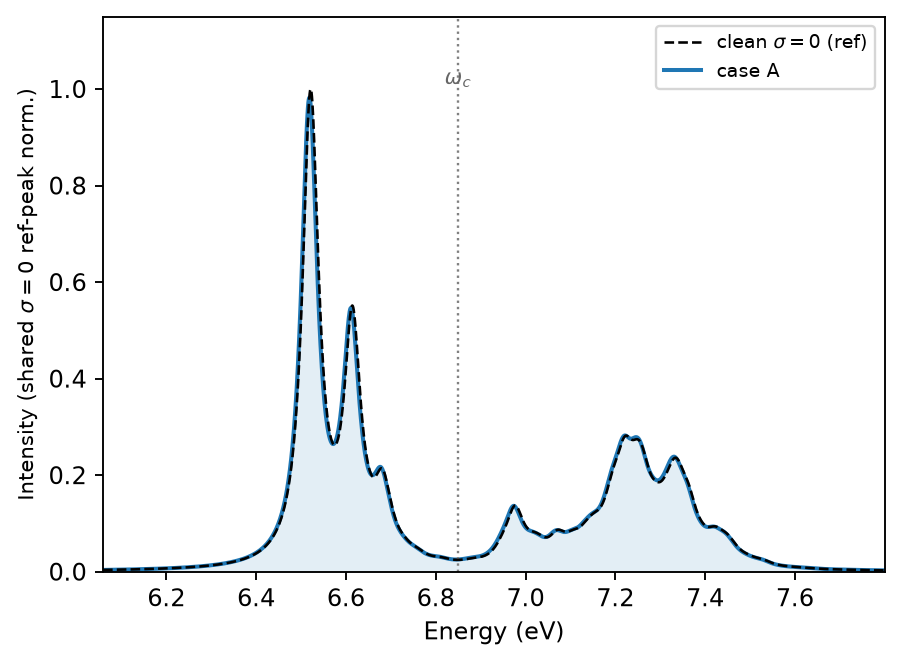
\includegraphics[width=0.39\textwidth]{fig_case_A_spec.png}\hfill
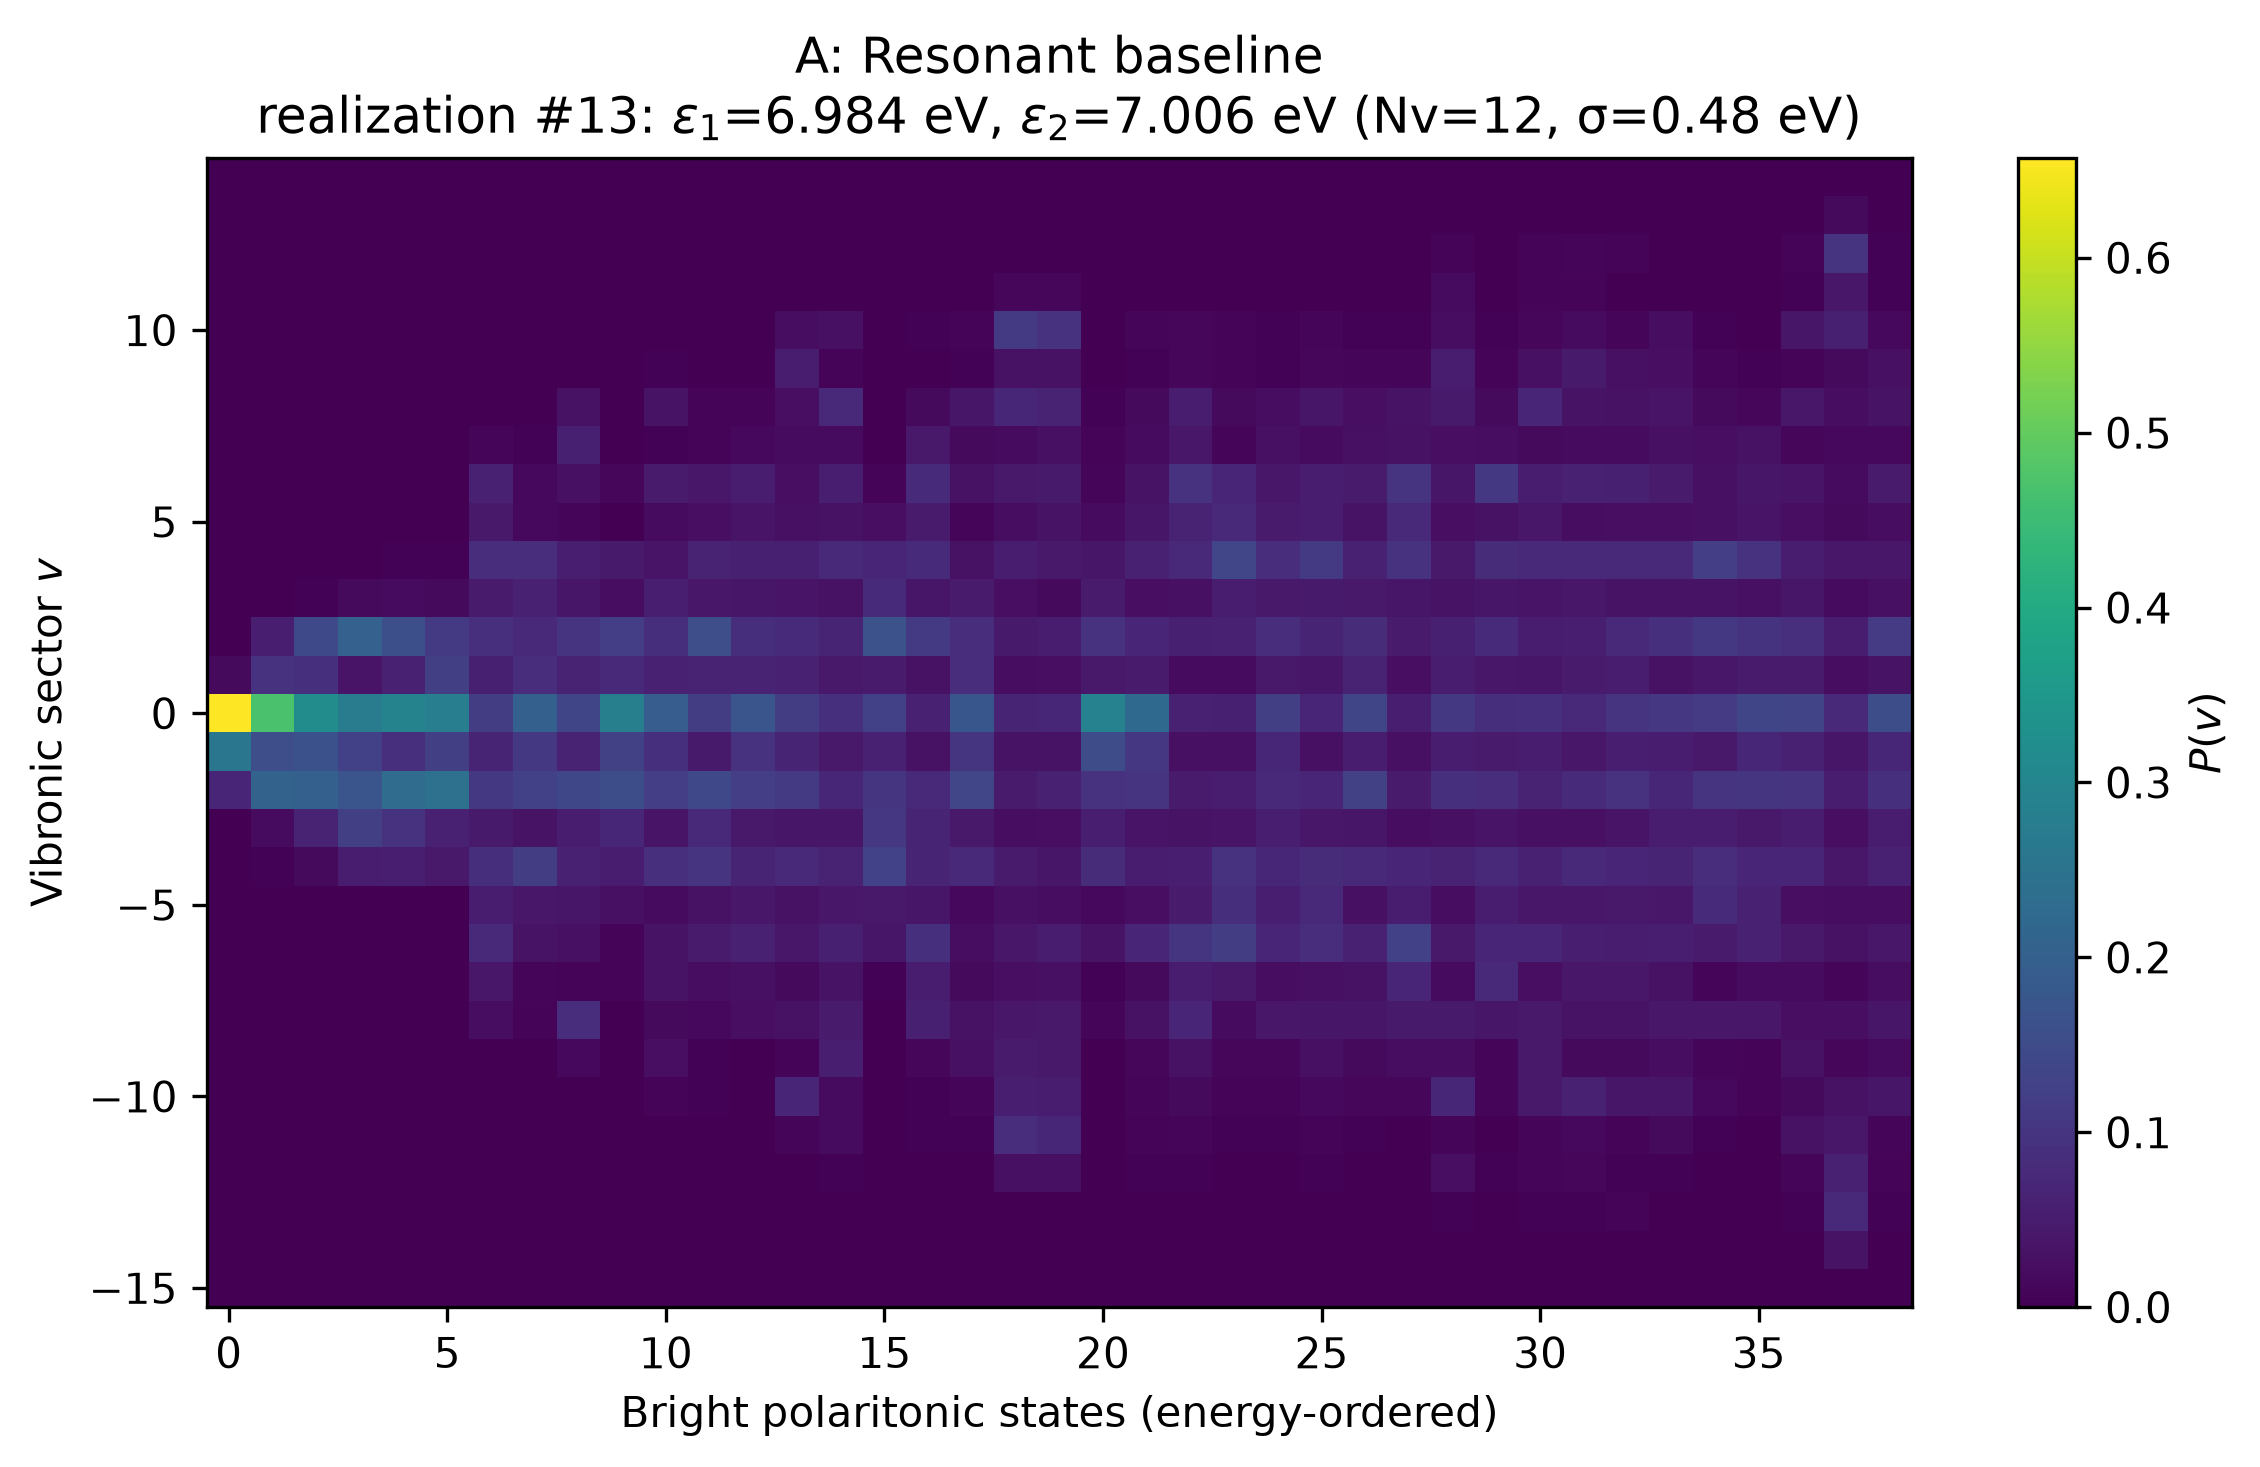
\includegraphics[width=0.44\textwidth]{fig_case_A_heatmap.png}
\caption{\textbf{Case A}, $(\epsilon_1,\epsilon_2)=(6.984,7.006)$.
\emph{Left:} absorption spectrum (blue) against the clean $\sigma=0$
reference (dashed). \emph{Right:} $P(v)$ heatmap of the bright polaritonic
states.}
\label{fig:caseA}
\end{figure}
\FloatBarrier

Both molecules are drawn essentially on resonance and matched
($\Delta=0.02$, $s\approx0$; Fig.~\ref{fig:caseA}). The spectrum reproduces
the clean one peak for peak (LP at $6.518$~eV with shoulders at $6.611$,
$6.676$~eV; UP triplet at $7.222$, $7.247$, $7.331$~eV), and the heatmap gives
$39$ bright states, $\PR_{\max}=20.6$, $v\in[-14,13]$, against $42$, $19.9$,
$[-14,13]$ for the clean reference. Case A is thus an internal control: the
disorder machinery leaves the clean physics intact, and it anchors every other
comparison.

\subsection{Cases D and E - moving both molecules together}

\begin{figure}[htbp]
\centering
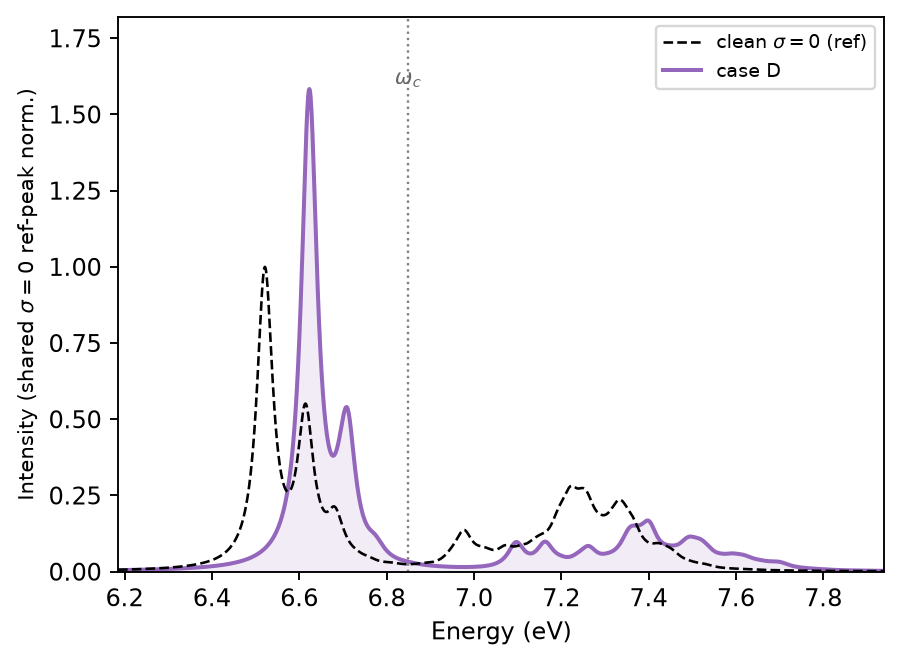
\includegraphics[width=0.39\textwidth]{fig_case_D_spec.png}\hfill
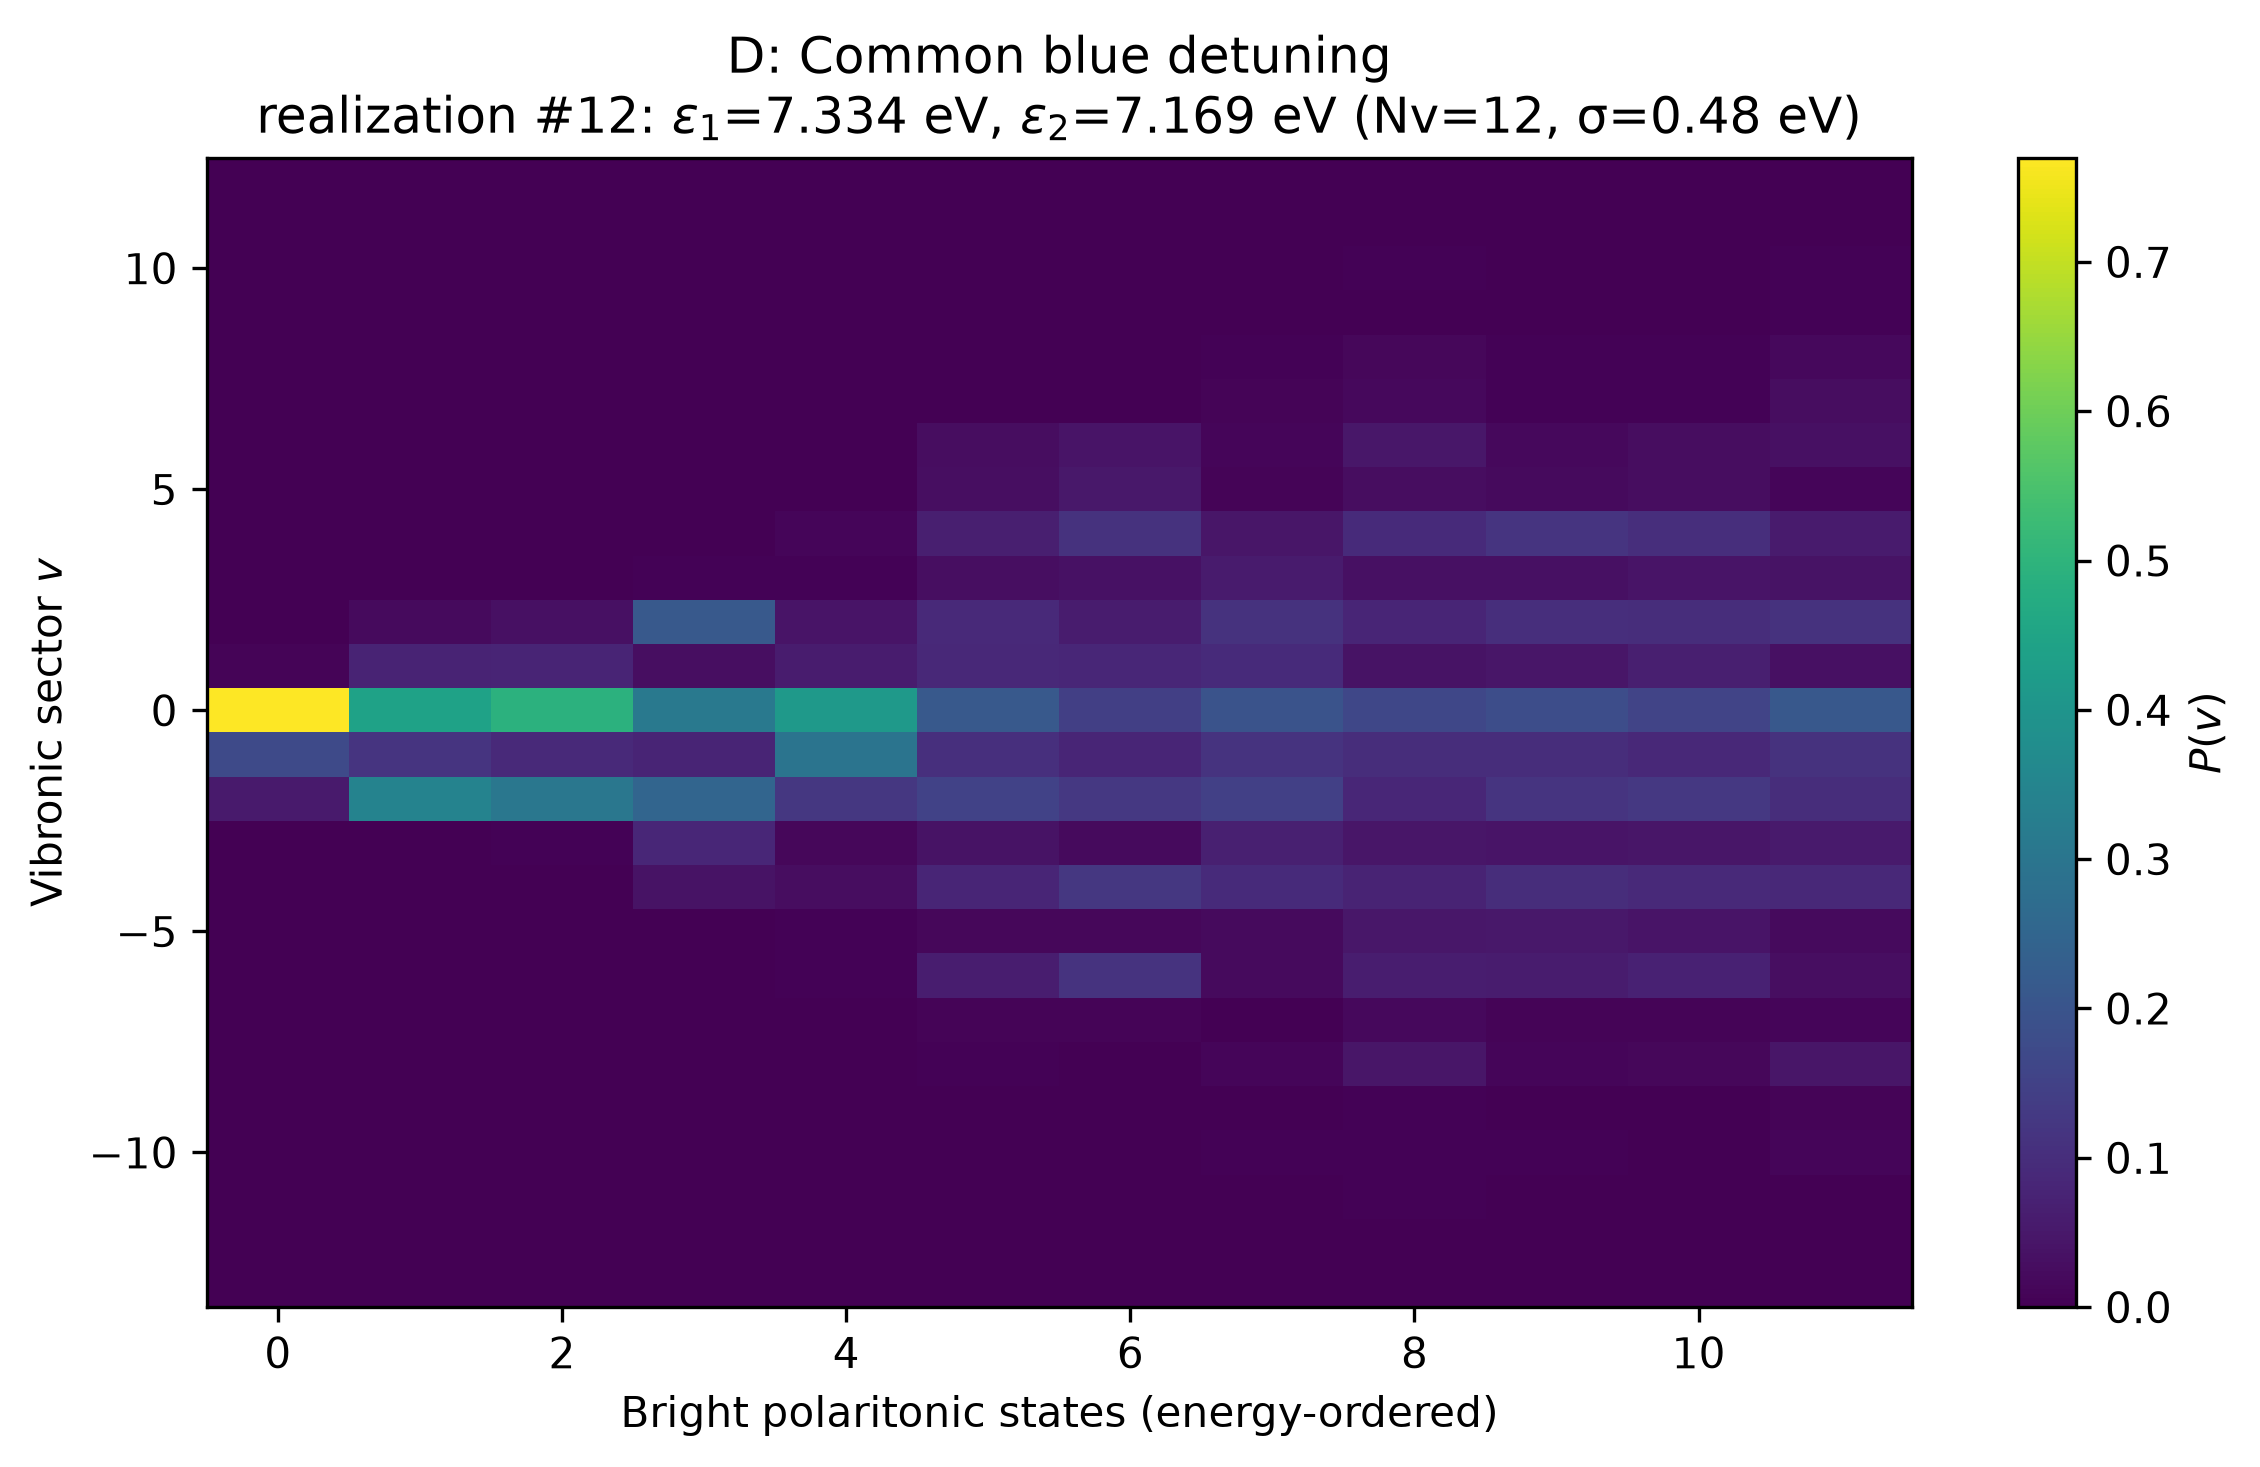
\includegraphics[width=0.44\textwidth]{fig_case_D_heatmap.png}\\[0.4em]
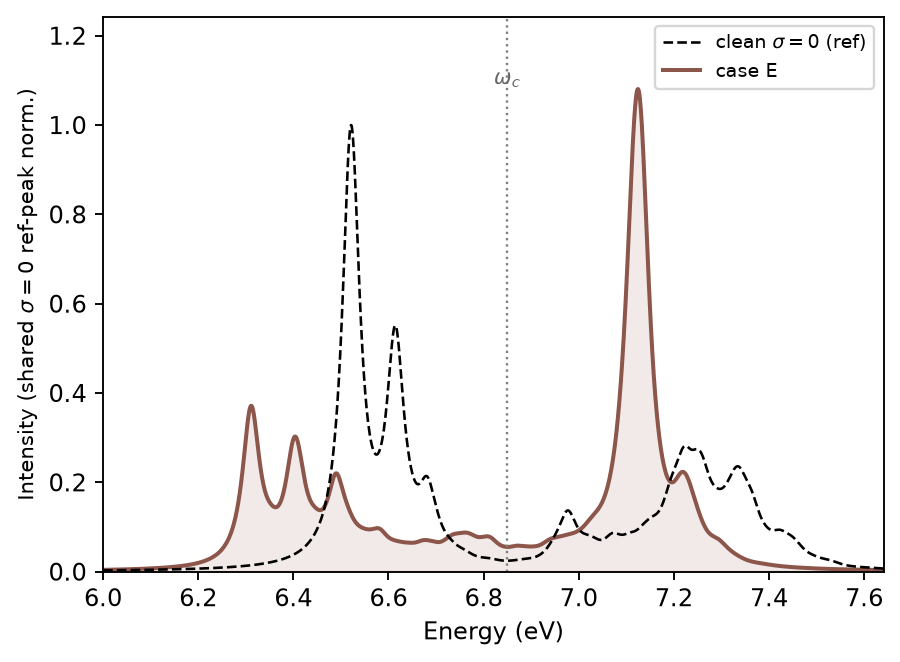
\includegraphics[width=0.39\textwidth]{fig_case_E_spec.png}\hfill
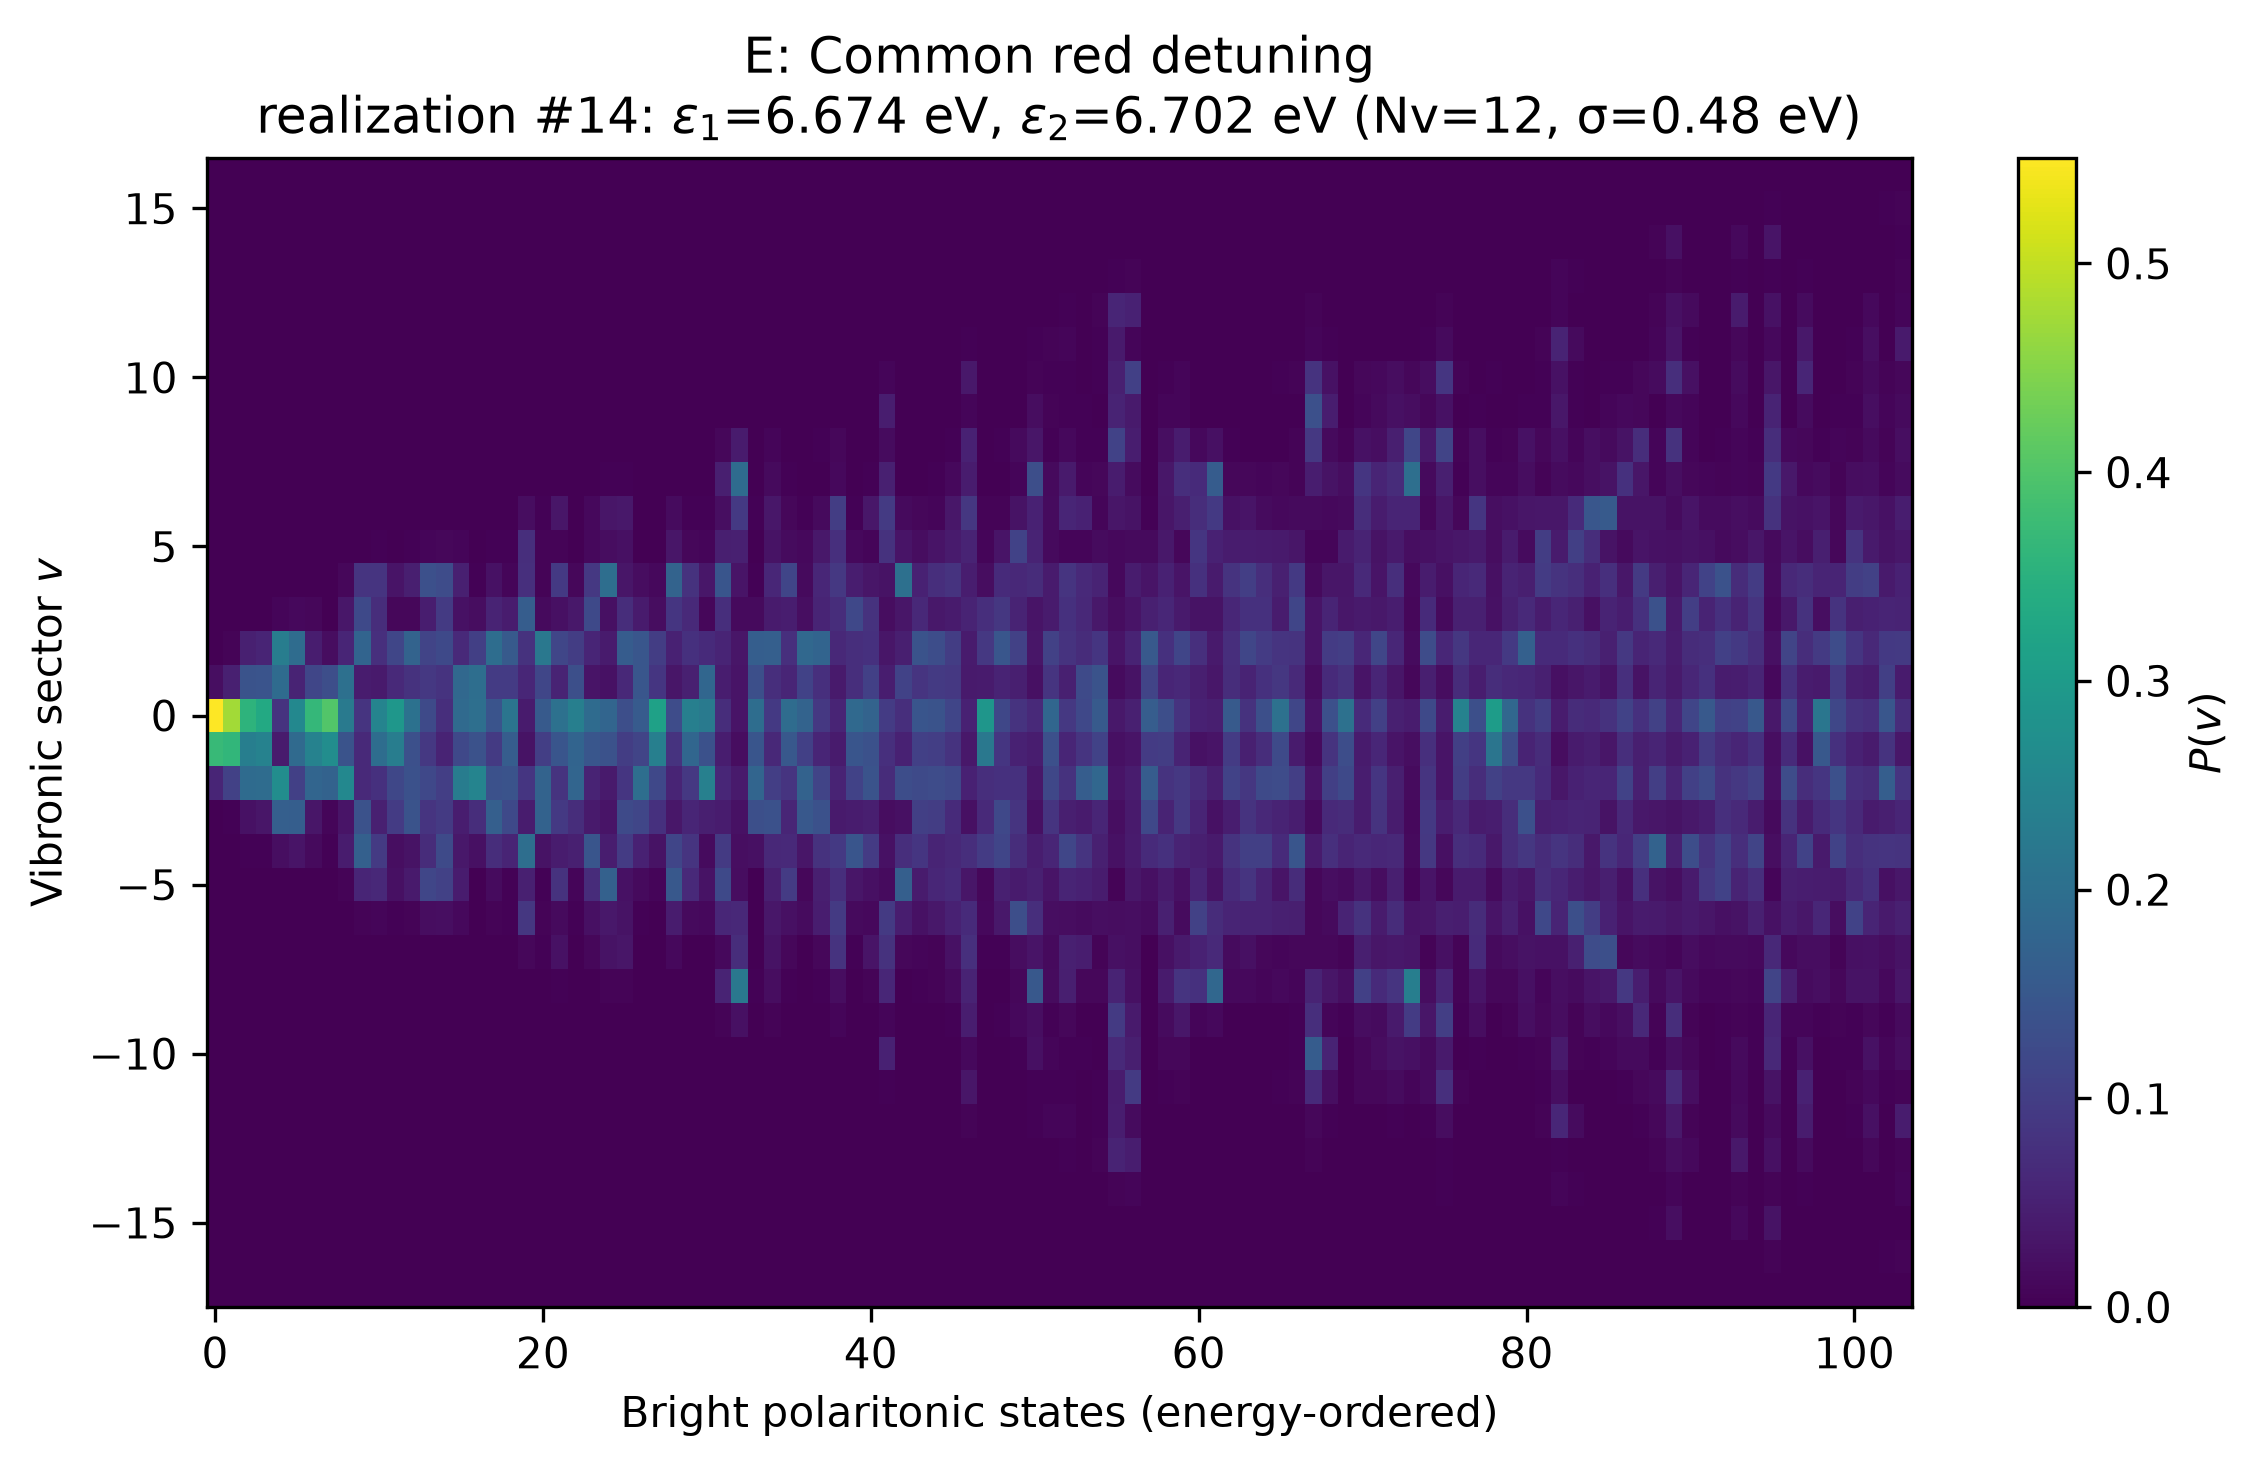
\includegraphics[width=0.44\textwidth]{fig_case_E_heatmap.png}
\caption{\textbf{Top - Case D}, common blue detuning,
$(\epsilon_1,\epsilon_2)=(7.334,7.169)$, $s=+1.0g$.
\textbf{Bottom - Case E}, common red detuning,
$(\epsilon_1,\epsilon_2)=(6.674,6.702)$, $s=-1.3g$. Left: spectra against the
clean reference (dashed); right: $P(v)$ heatmaps.}
\label{fig:caseDE}
\end{figure}
\FloatBarrier

Cases D and E (Fig.~\ref{fig:caseDE}) keep the two molecules matched
($\Delta$ small) but shift them together, blue by $s=+1.0g$ and red by
$s=-1.3g$. They are nominally mirror images, but they
are \emph{not} physically equivalent.

In \textbf{Case D} the spectrum blue-shifts and collapses to two resolved LP
peaks ($6.623$, $6.708$~eV) with the UP pushed up to $\approx7.37$~eV; only
$12$ states stay bright, $\PR_{\max}$ drops to $12.5$ and the range narrows to
$v\in[-8,8]$ - the cascade is reduced to roughly $60\%$ of baseline. In
\textbf{Case E} the whole spectrum red-shifts (LP cluster at $6.311$, $6.404$,
$6.490$~eV) and the UP feature at $7.125$~eV becomes the \emph{brightest}
peak, inverting the oscillator-strength ordering of A. Its heatmap is the
richest of all eight cases: $104$ bright states ($2.6\times$ the clean
reference), $\PR_{\max}=22.4$, and the widest range $v\in[-15,14]$.

Here is a more direct way to see why. Since the molecules stay matched, the
shifted pair still behaves as a single unit detuned from the cavity by $s$,
and a detuned molecule--cavity system always splits into two branches: one
that tracks the molecule's own (shifted) energy and keeps its full JT
vibronic structure, and one that stays closer to $\omega_c$ and is mostly
photon in character. How rich each branch looks in absorption then depends on
how much of the bare JT vibronic manifold (Fig.~\ref{fig:1mol}, whose density
is not symmetric about $\epsilon$) sits close enough to the molecule-like
branch to borrow some of its photon weight. E's red shift moves its
molecule-like branch down into a denser stretch of that bare structure, so
many nearby vibronic sub-levels borrow enough photon weight to cross the
brightness threshold - giving the richest heatmap of the eight cases. D's
blue shift moves its molecule-like branch up into a sparser stretch instead,
so far fewer sub-levels light up, while the photon-like branch left behind
near $\omega_c$ contributes only the two simple peaks seen in
Fig.~\ref{fig:caseDE}. Case E is the cavity-JT realisation of the
disorder-\emph{enhanced} regime of
Ref.~\cite{Wellnitz2022}, which peaks when the offset is of order $g_c$.

\subsection{Cases F, H, C and B - breaking the symmetry between molecules}

\begin{figure}[htbp]
\centering
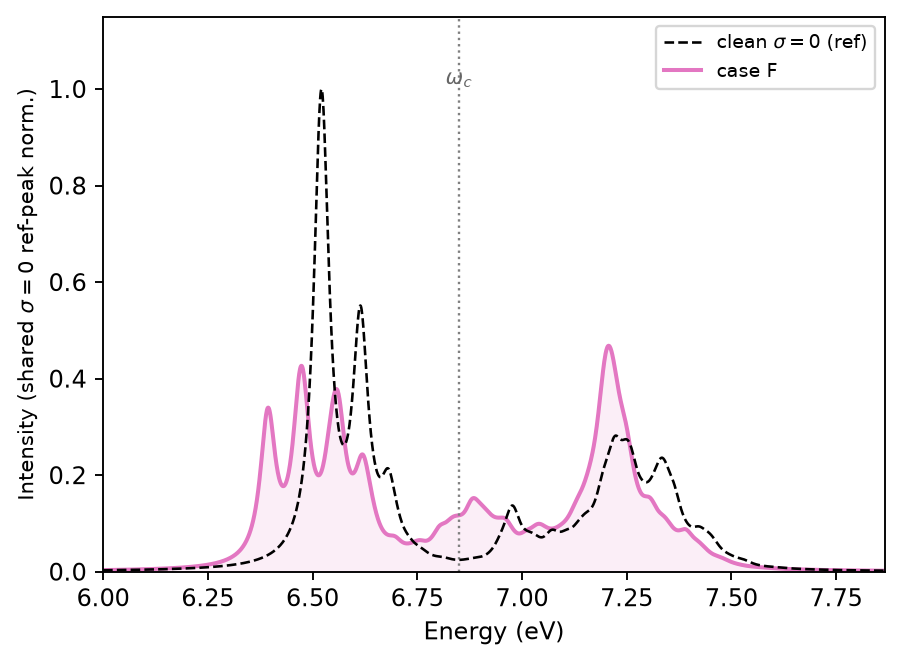
\includegraphics[width=0.39\textwidth]{fig_case_F_spec.png}\hfill
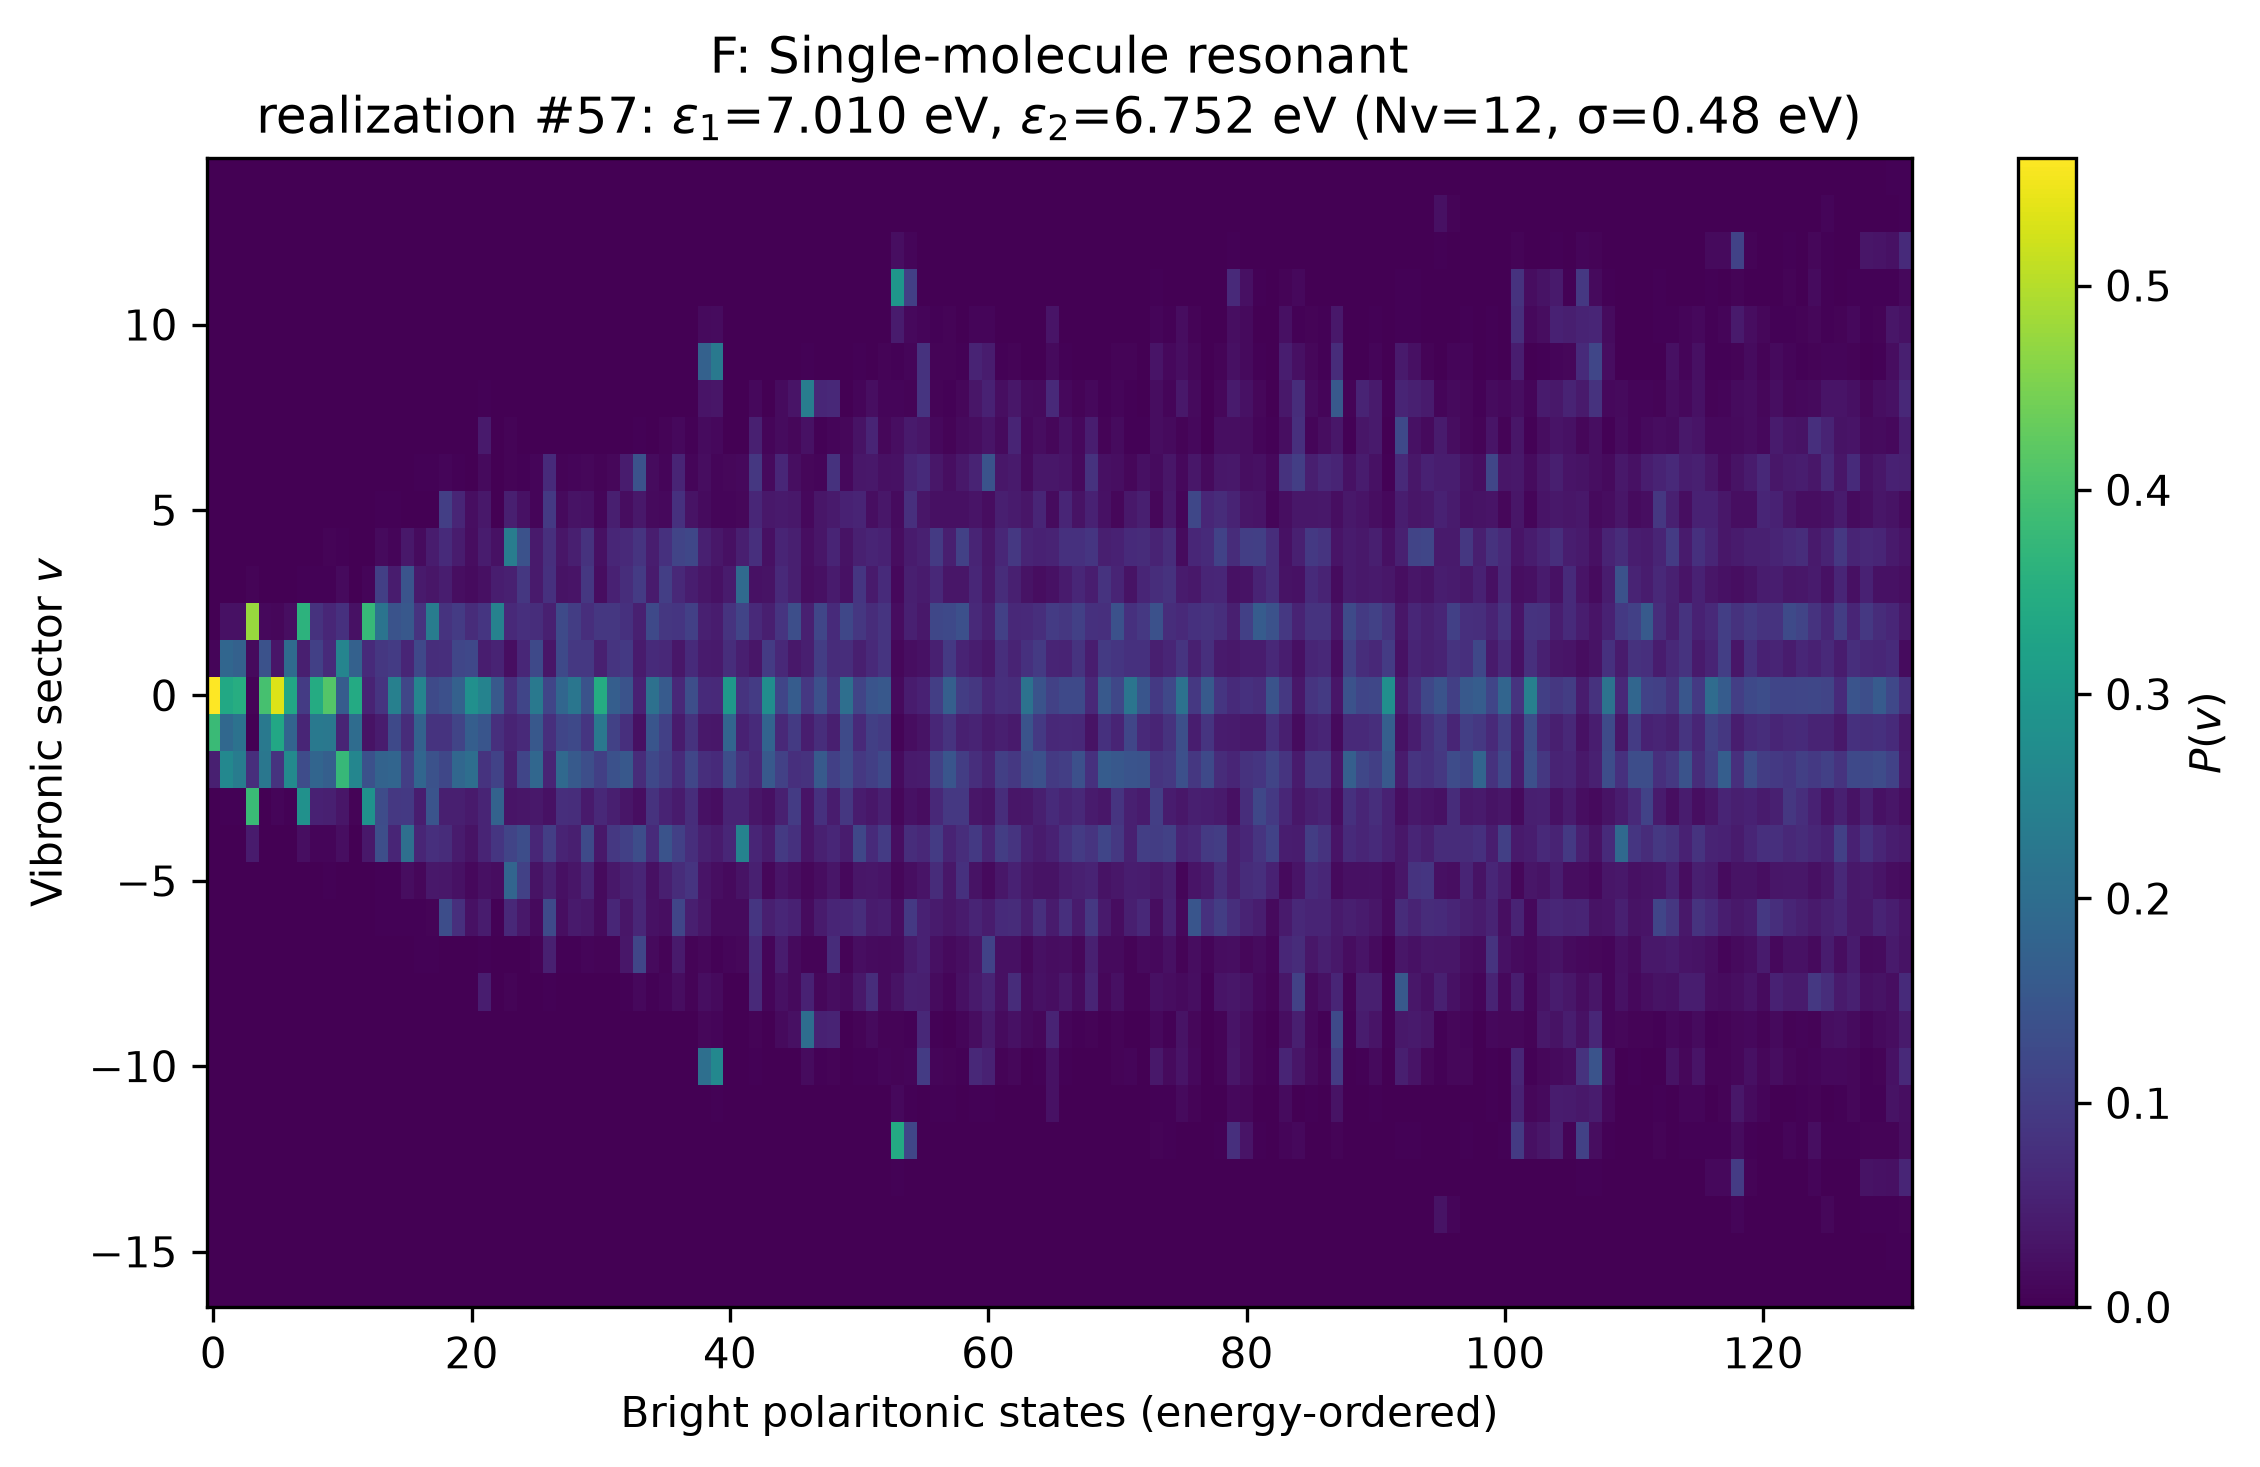
\includegraphics[width=0.44\textwidth]{fig_case_F_heatmap.png}\\[0.4em]
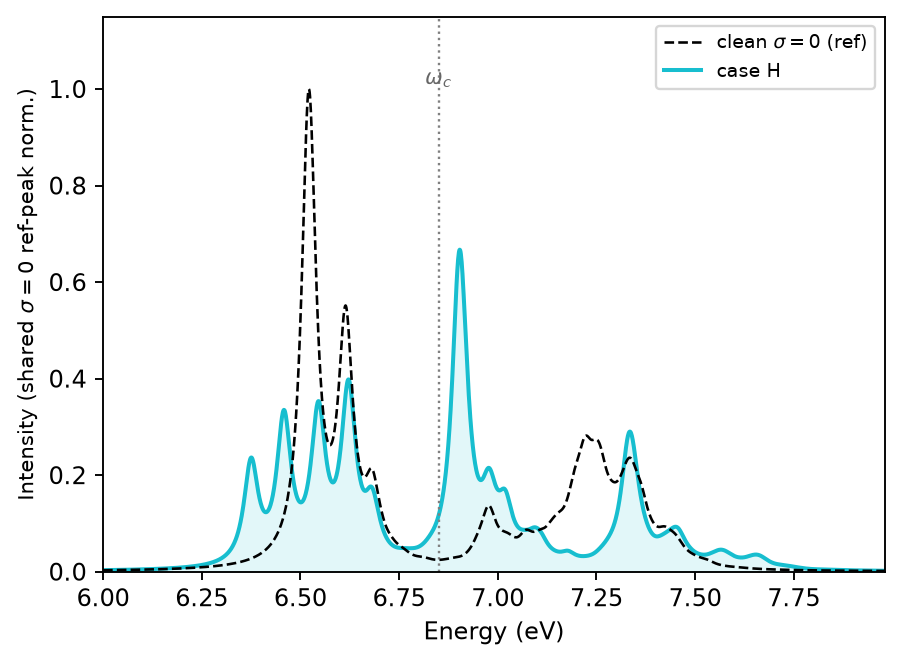
\includegraphics[width=0.39\textwidth]{fig_case_H_spec.png}\hfill
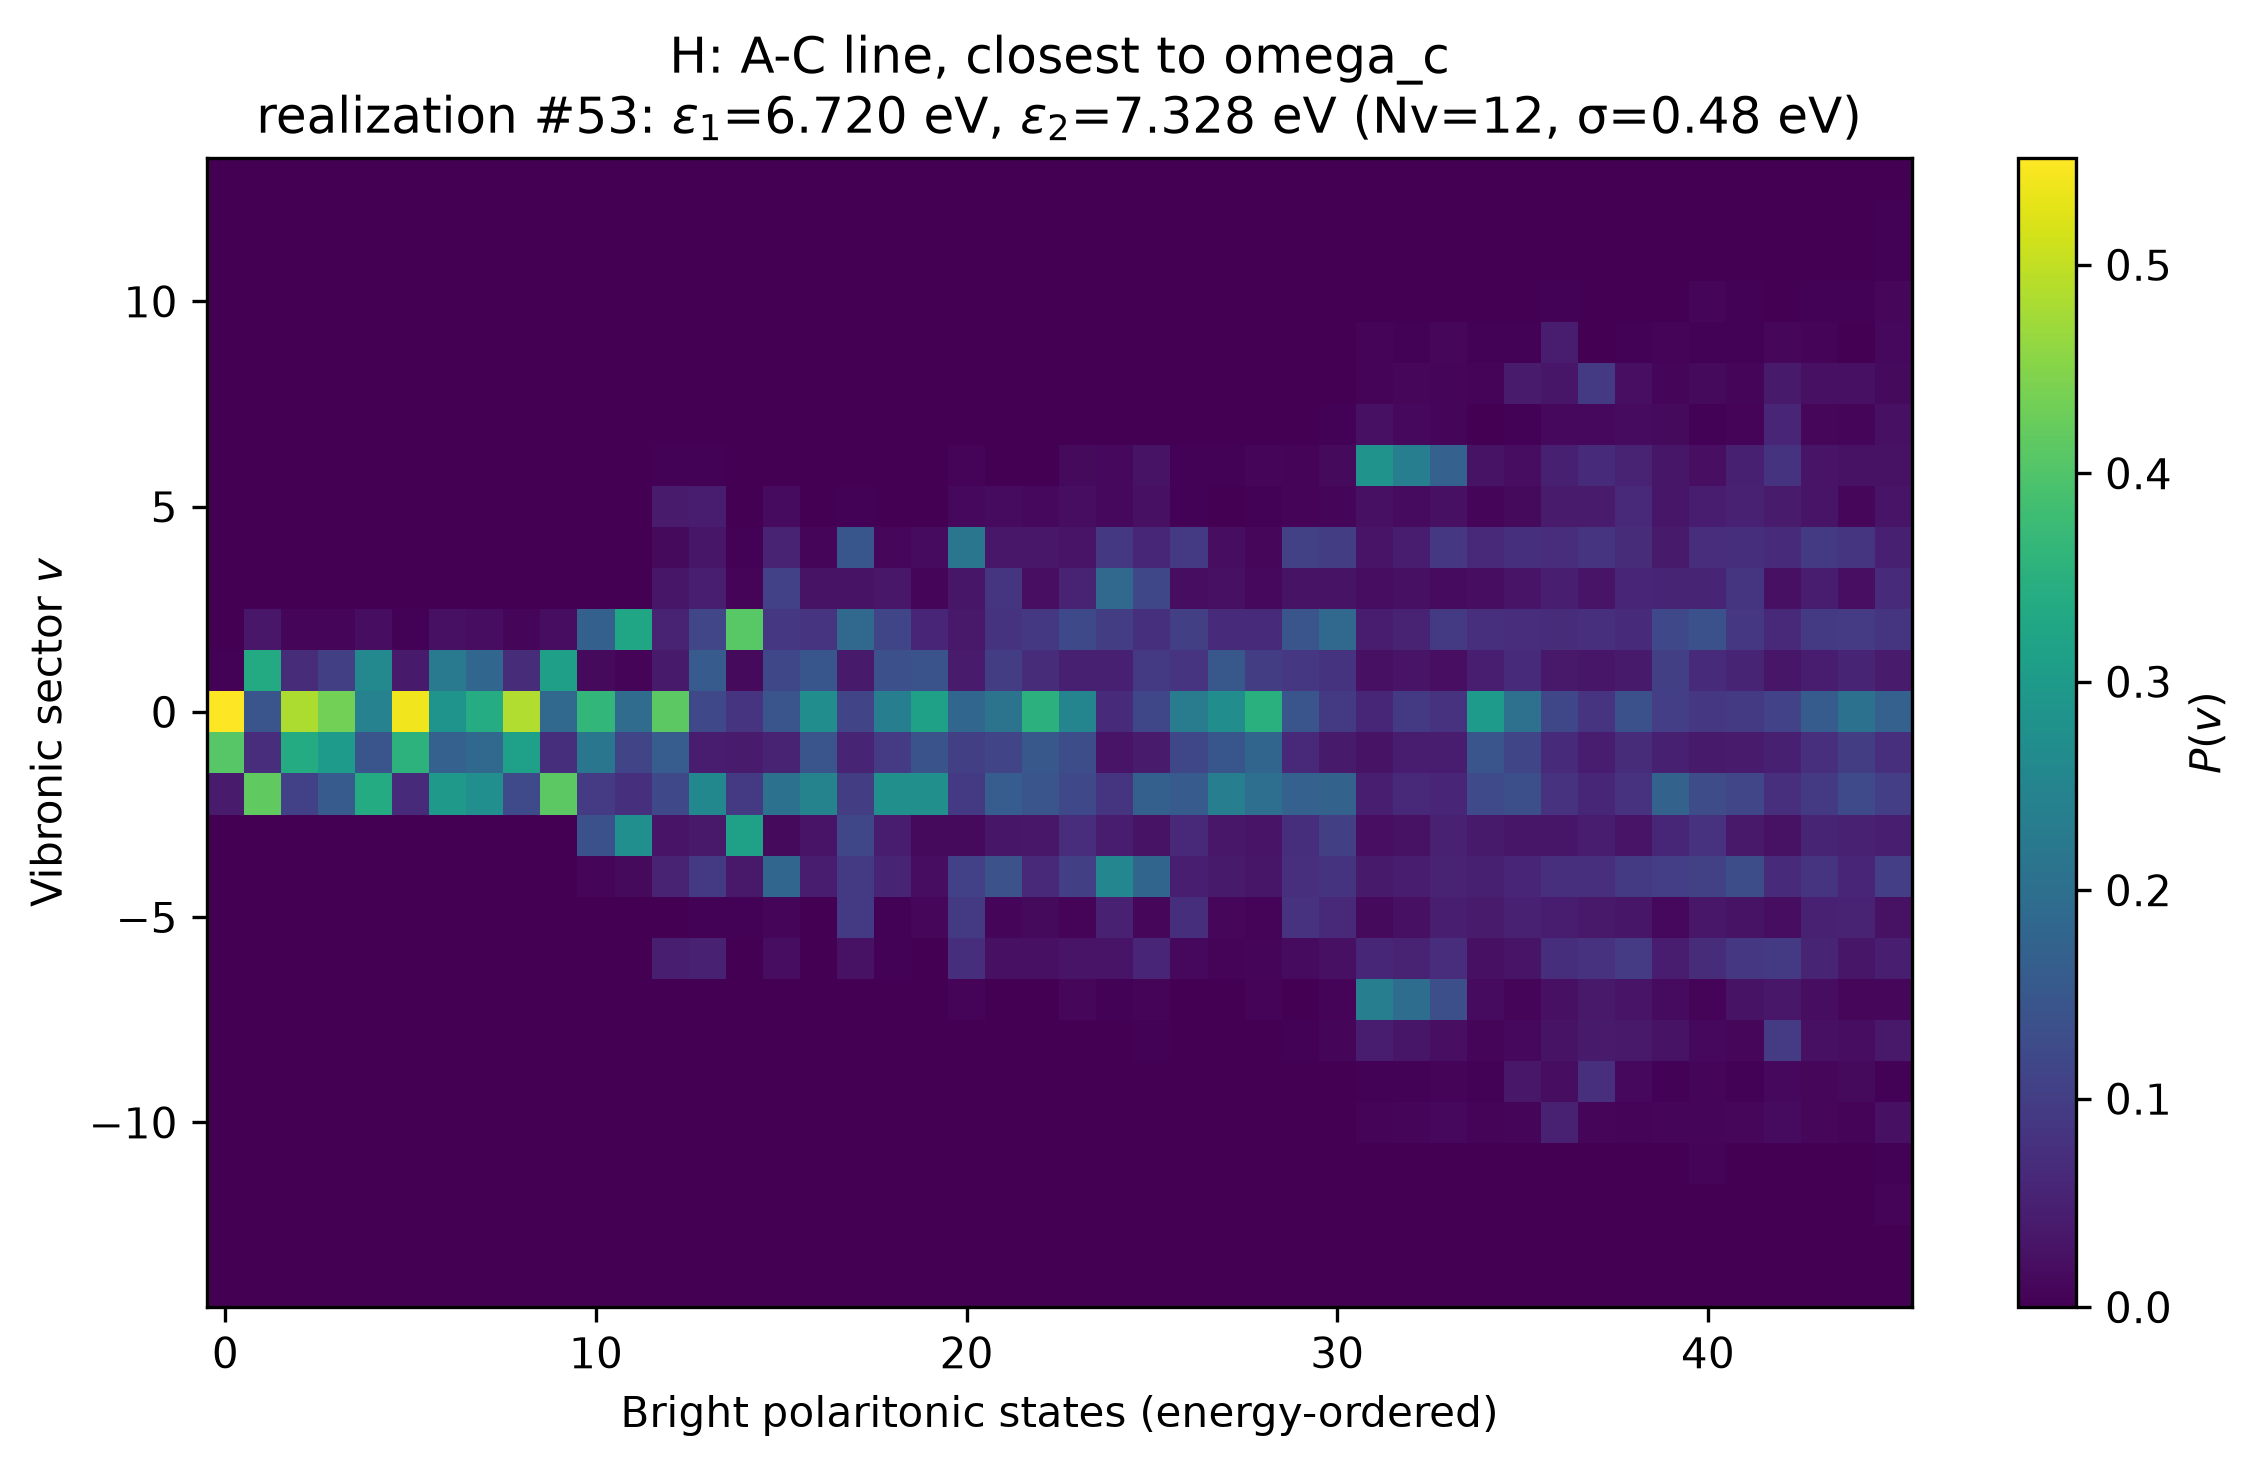
\includegraphics[width=0.44\textwidth]{fig_case_H_heatmap.png}
\caption{\textbf{Top - Case F}, single-molecule resonant,
$(\epsilon_1,\epsilon_2)=(7.010,6.752)$, $\Delta=g$.
\textbf{Bottom - Case H}, interior point of the A--C line (opposite
disorder), $(\epsilon_1,\epsilon_2)=(6.720,7.328)$, $\Delta=2.5g$, $s\approx0$.}
\label{fig:caseFH}
\end{figure}
\FloatBarrier

\textbf{Case F} (Fig.~\ref{fig:caseFH}, top) introduces a genuine
inter-molecular mismatch of exactly one coupling, $\Delta=g$: one molecule is brought back onto resonance
($\delta_1\approx0$) while the other stays detuned by $-g$. With
$\Delta\approx g$ the system sits right at the crossover and the two molecules
still hybridise collectively: $132$ bright states result - the most of any case -
with $\PR_{\max}=21.6$ and $v\in[-14,13]$. The spectrum is correspondingly
the most structured of the set: ten resolved features spread from $6.39$ to
$7.39$~eV, with the UP peak at $7.207$~eV the brightest and the LP cluster
($6.394$, $6.473$, $6.557$, $6.619$~eV) carrying $50$--$90\%$ of it, so the
oscillator strength is spread out rather than concentrated.

\textbf{Case H} was constructed on the line joining A and C in the
$(\epsilon_1,\epsilon_2)$ plane - the $s\approx0$ anti-diagonal along which
the two molecules are detuned \emph{oppositely} - at the interior point
closest to $\omega_c$. Here $\Delta=2.5g$ with $s\approx0$. The result is
mixed: $46$ bright states, \emph{more} than A's $39$, so the
opposite-disorder mismatch produces more peaks
in absorption; but $\PR_{\max}=16.2$ and $v\in[-10,9]$, both \emph{below} A.
Disorder here simultaneously exposes more of the manifold and degrades the
spread of each individual state. The brightest peak sits at $6.903$~eV,
essentially at $\omega_c$, with oscillator strength spread across the whole
band instead of concentrated in one polariton.

\begin{figure}[htbp]
\centering
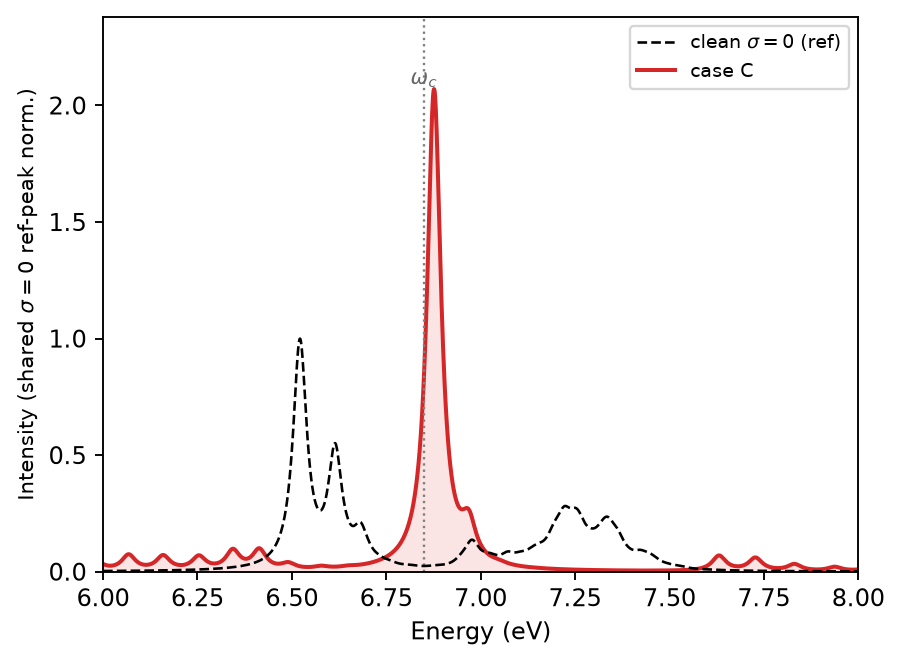
\includegraphics[width=0.39\textwidth]{fig_case_C_spec.png}\hfill
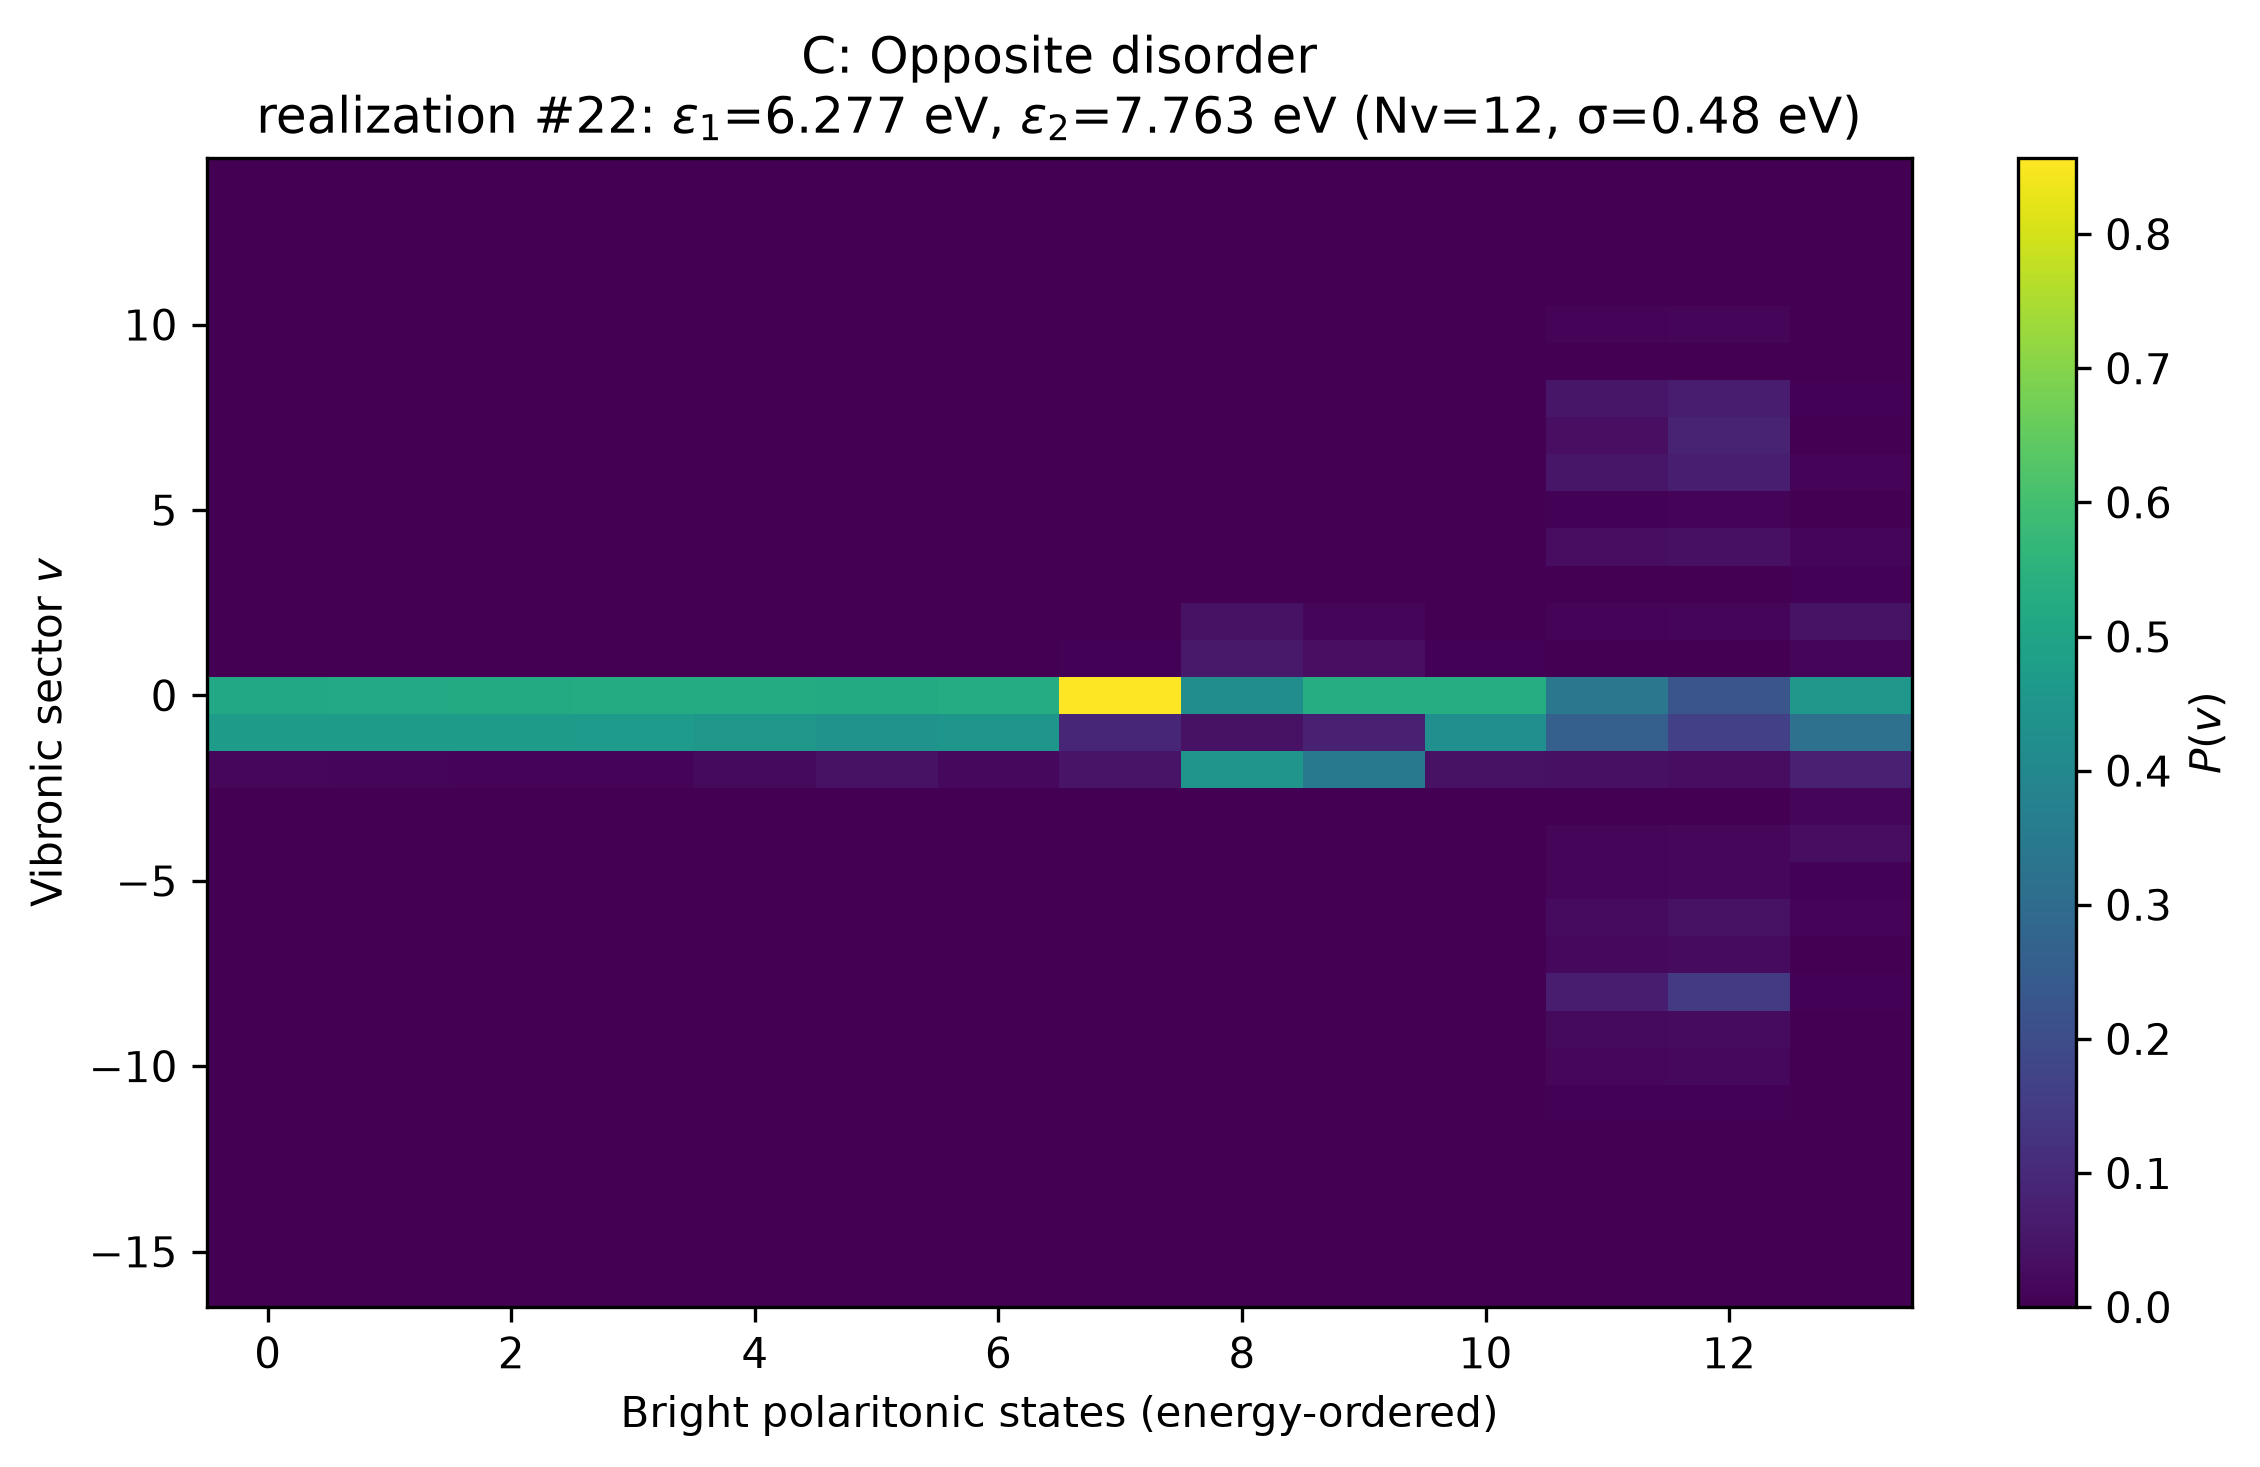
\includegraphics[width=0.44\textwidth]{fig_case_C_heatmap.png}\\[0.4em]
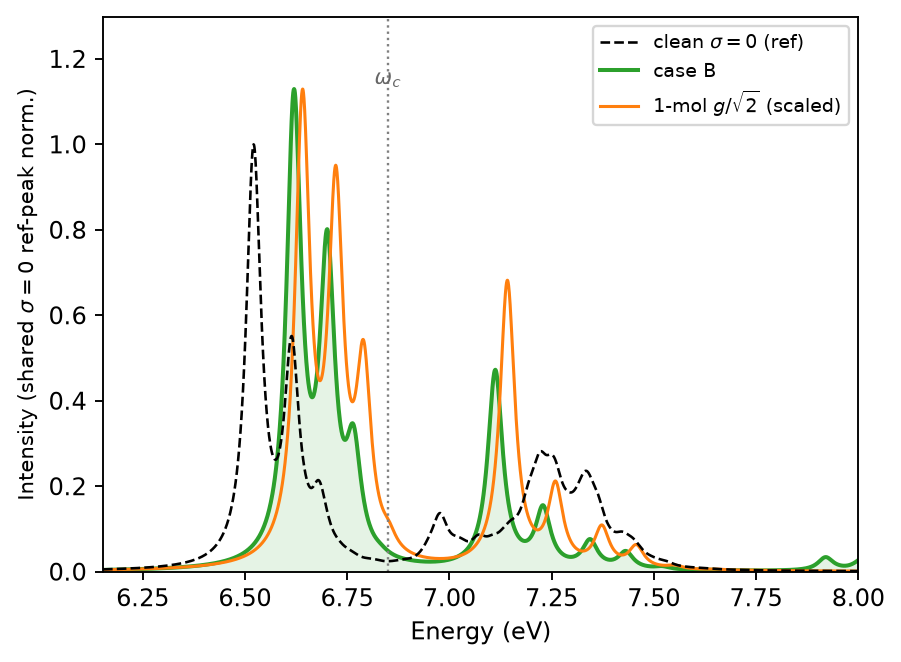
\includegraphics[width=0.39\textwidth]{fig_case_B_spec.png}\hfill
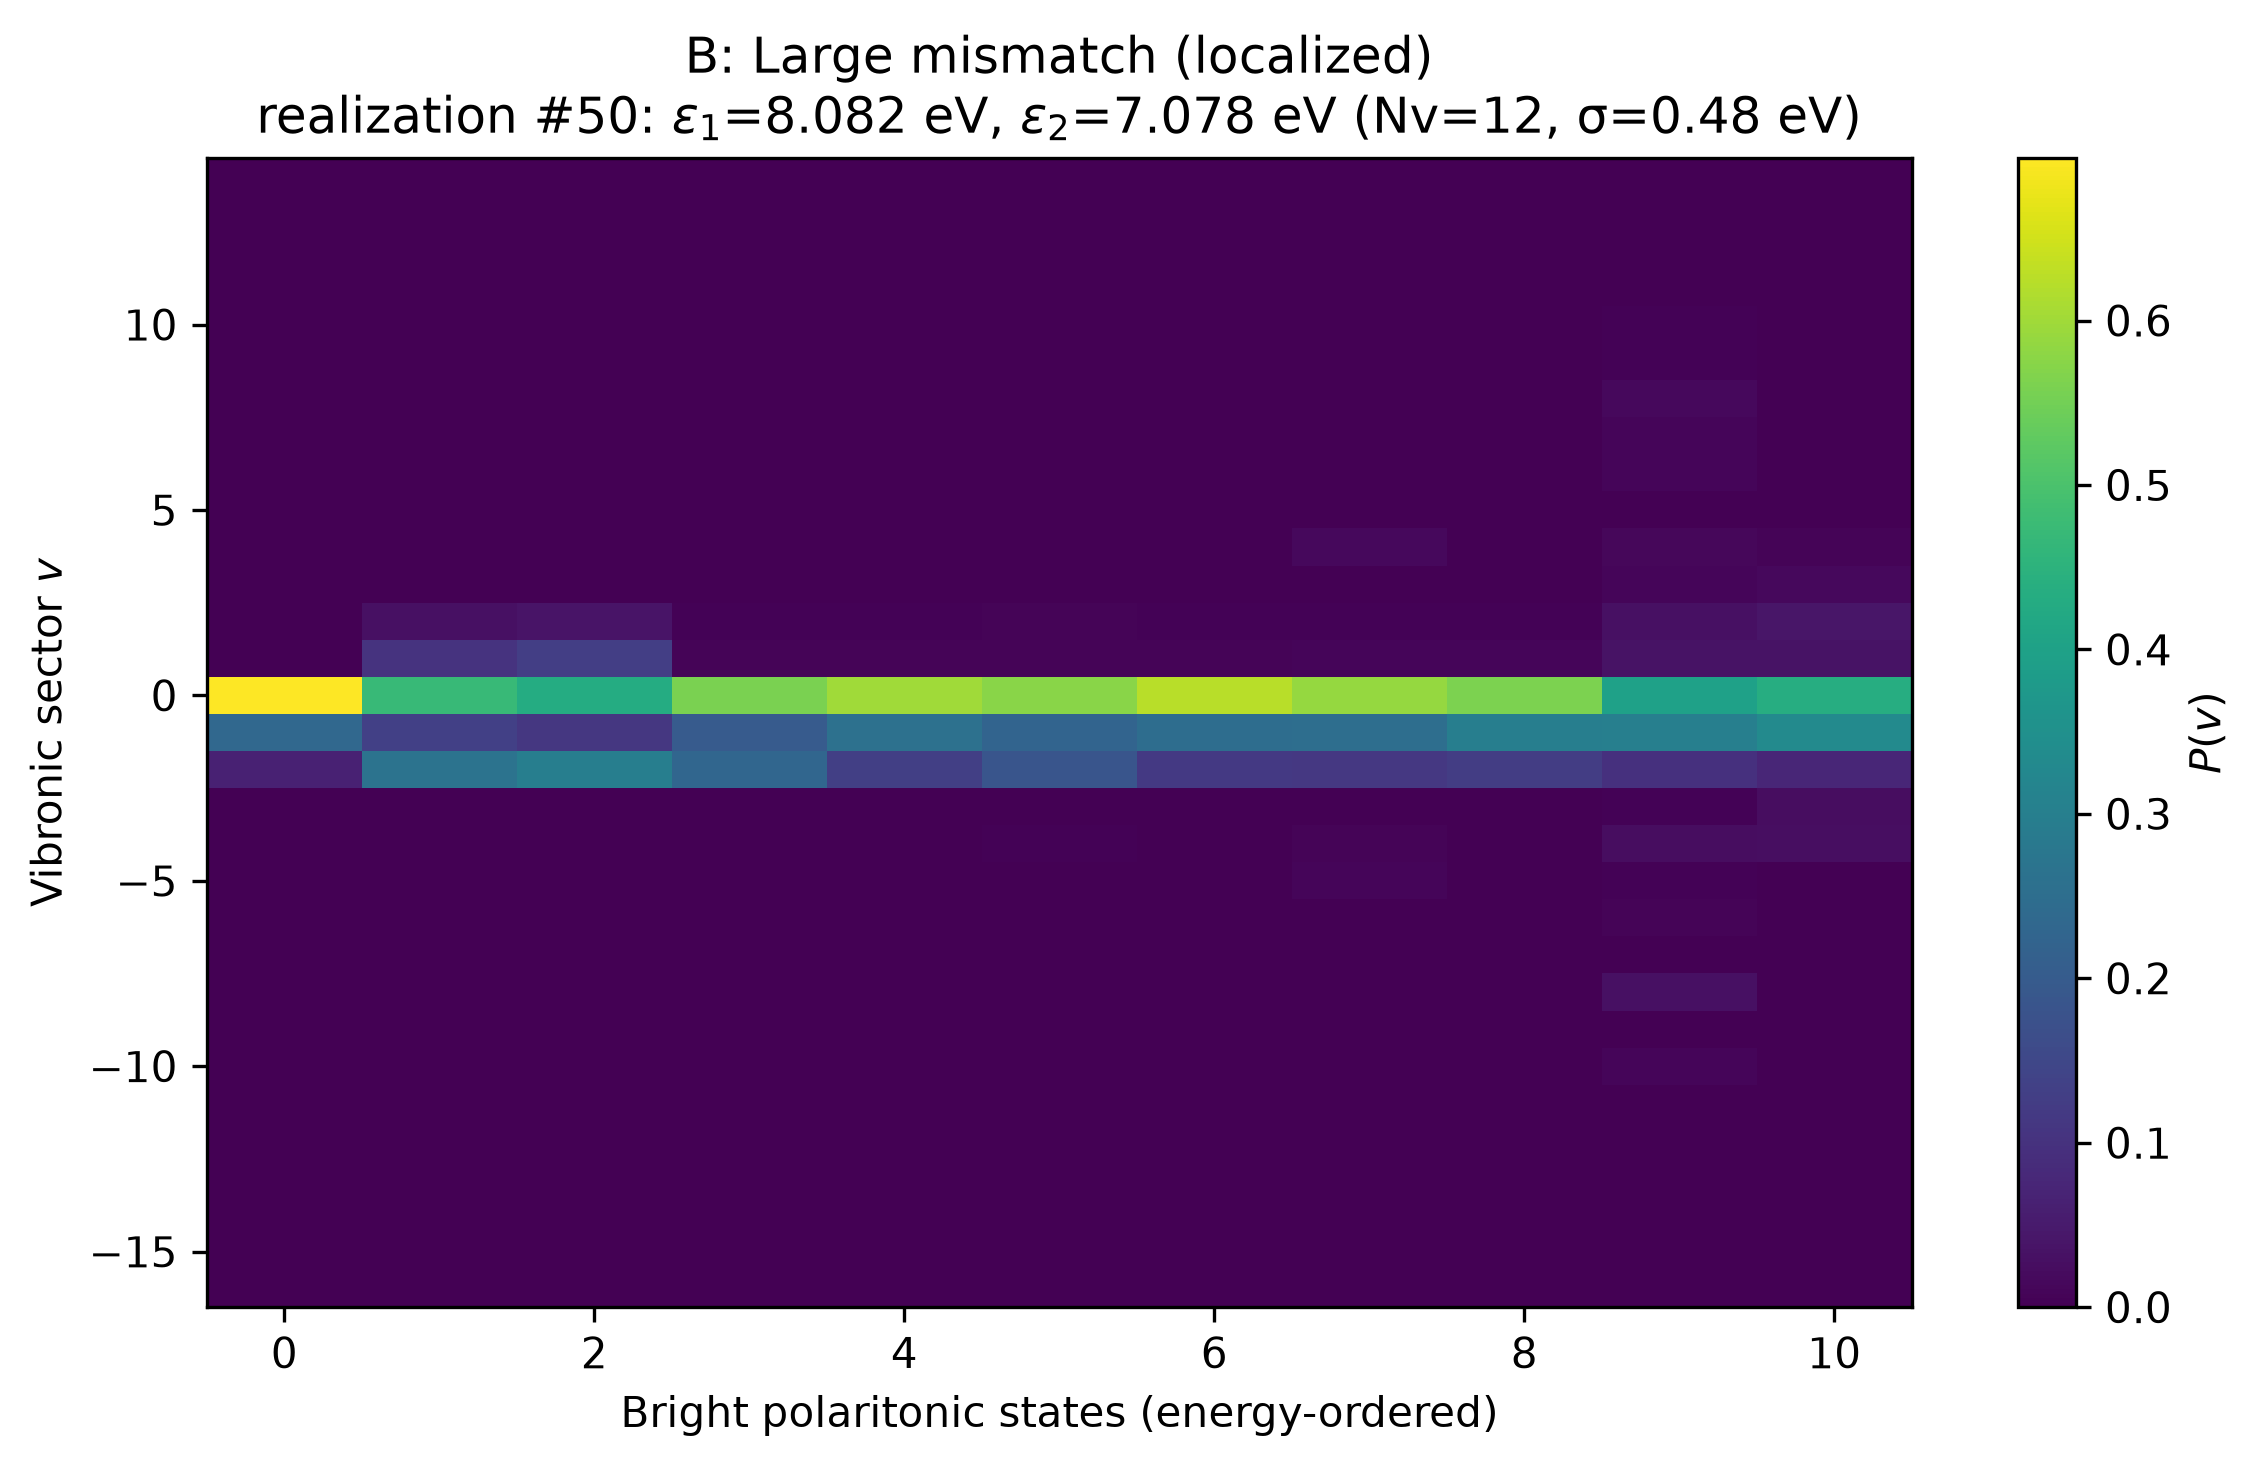
\includegraphics[width=0.44\textwidth]{fig_case_B_heatmap.png}
\caption{\textbf{Top - Case C}, opposite disorder pushed far out along the
A--C line, $(\epsilon_1,\epsilon_2)=(6.277,7.763)$, $\Delta=6g$, $s\approx0$.
\textbf{Bottom - Case B}, large same-side mismatch,
$(\epsilon_1,\epsilon_2)=(8.082,7.078)$, $\Delta=4g$, $s=+2.4g$; the orange
curve is a single-molecule JT polariton spectrum computed at $g/\sqrt2$ for
comparison.}
\label{fig:caseCB}
\end{figure}
\FloatBarrier

\textbf{Case C} continues along the same A--H--C line to $\Delta=6g$. Both
molecules have now left the bright line, in opposite directions, and the
spectrum collapses onto a single dominant peak at $6.876$~eV - essentially
the bare cavity photon. Only $14$ states are bright, $\PR_{\max}$ falls to
$8.5$, and the $P(v)$ weight is mostly pinned to $v\in\{0,-1,-2\}$ with a faint
high-$v$ tail. Along A $\to$ H $\to$ C the cascade therefore weakens
monotonically, $\PR_{\max}: 20.6\to16.2\to8.5$, as the opposite-disorder
mismatch grows.

\textbf{Case B} takes the mismatch to the \emph{same} side instead: molecule 1
is detuned by $+4.5g$ while molecule 2 stays near resonance ($\Delta=4g\gg g$),
and the excitation \emph{localizes} entirely on the resonant molecule. The
spectrum is that of a \emph{single} JT polariton - LP at $6.620$~eV followed
by a clean vibrational progression at $6.701$, $6.763$~eV and one UP feature at
$7.113$~eV - and it overlays the independently computed one-molecule spectrum
at $g/\sqrt2$ (orange curve, Fig.~\ref{fig:caseCB}). The heatmap confirms
this: $11$ bright states, all with $P(v)$ confined to a flat horizontal band,
$\PR_{\max}=3.8$, i.e.\ the single-molecule bound of Sec.~\ref{sec:1mol}. Case
B is thus a direct, disorder-induced crossover from the collective physics of
Ref.~\cite{Pandit2025} back to the single-molecule physics of
Ref.~\cite{Nandipati2023}; its $11$ bright lines are a Franck--Condon
progression, not a cascade.

\subsection{Case G - bare-molecule limit}

\begin{figure}[htbp]
\centering
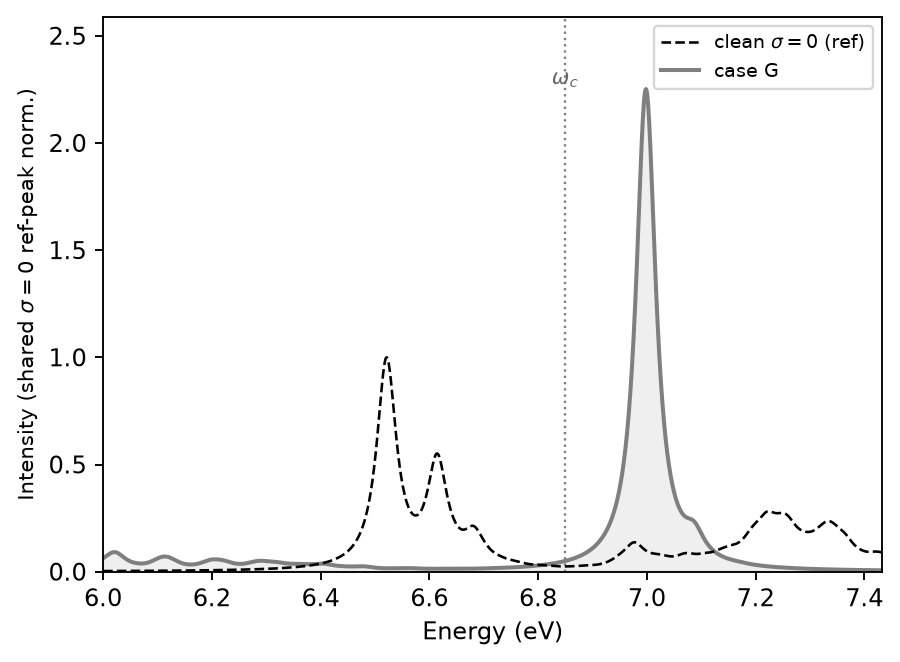
\includegraphics[width=0.39\textwidth]{fig_case_G_spec.png}\hfill
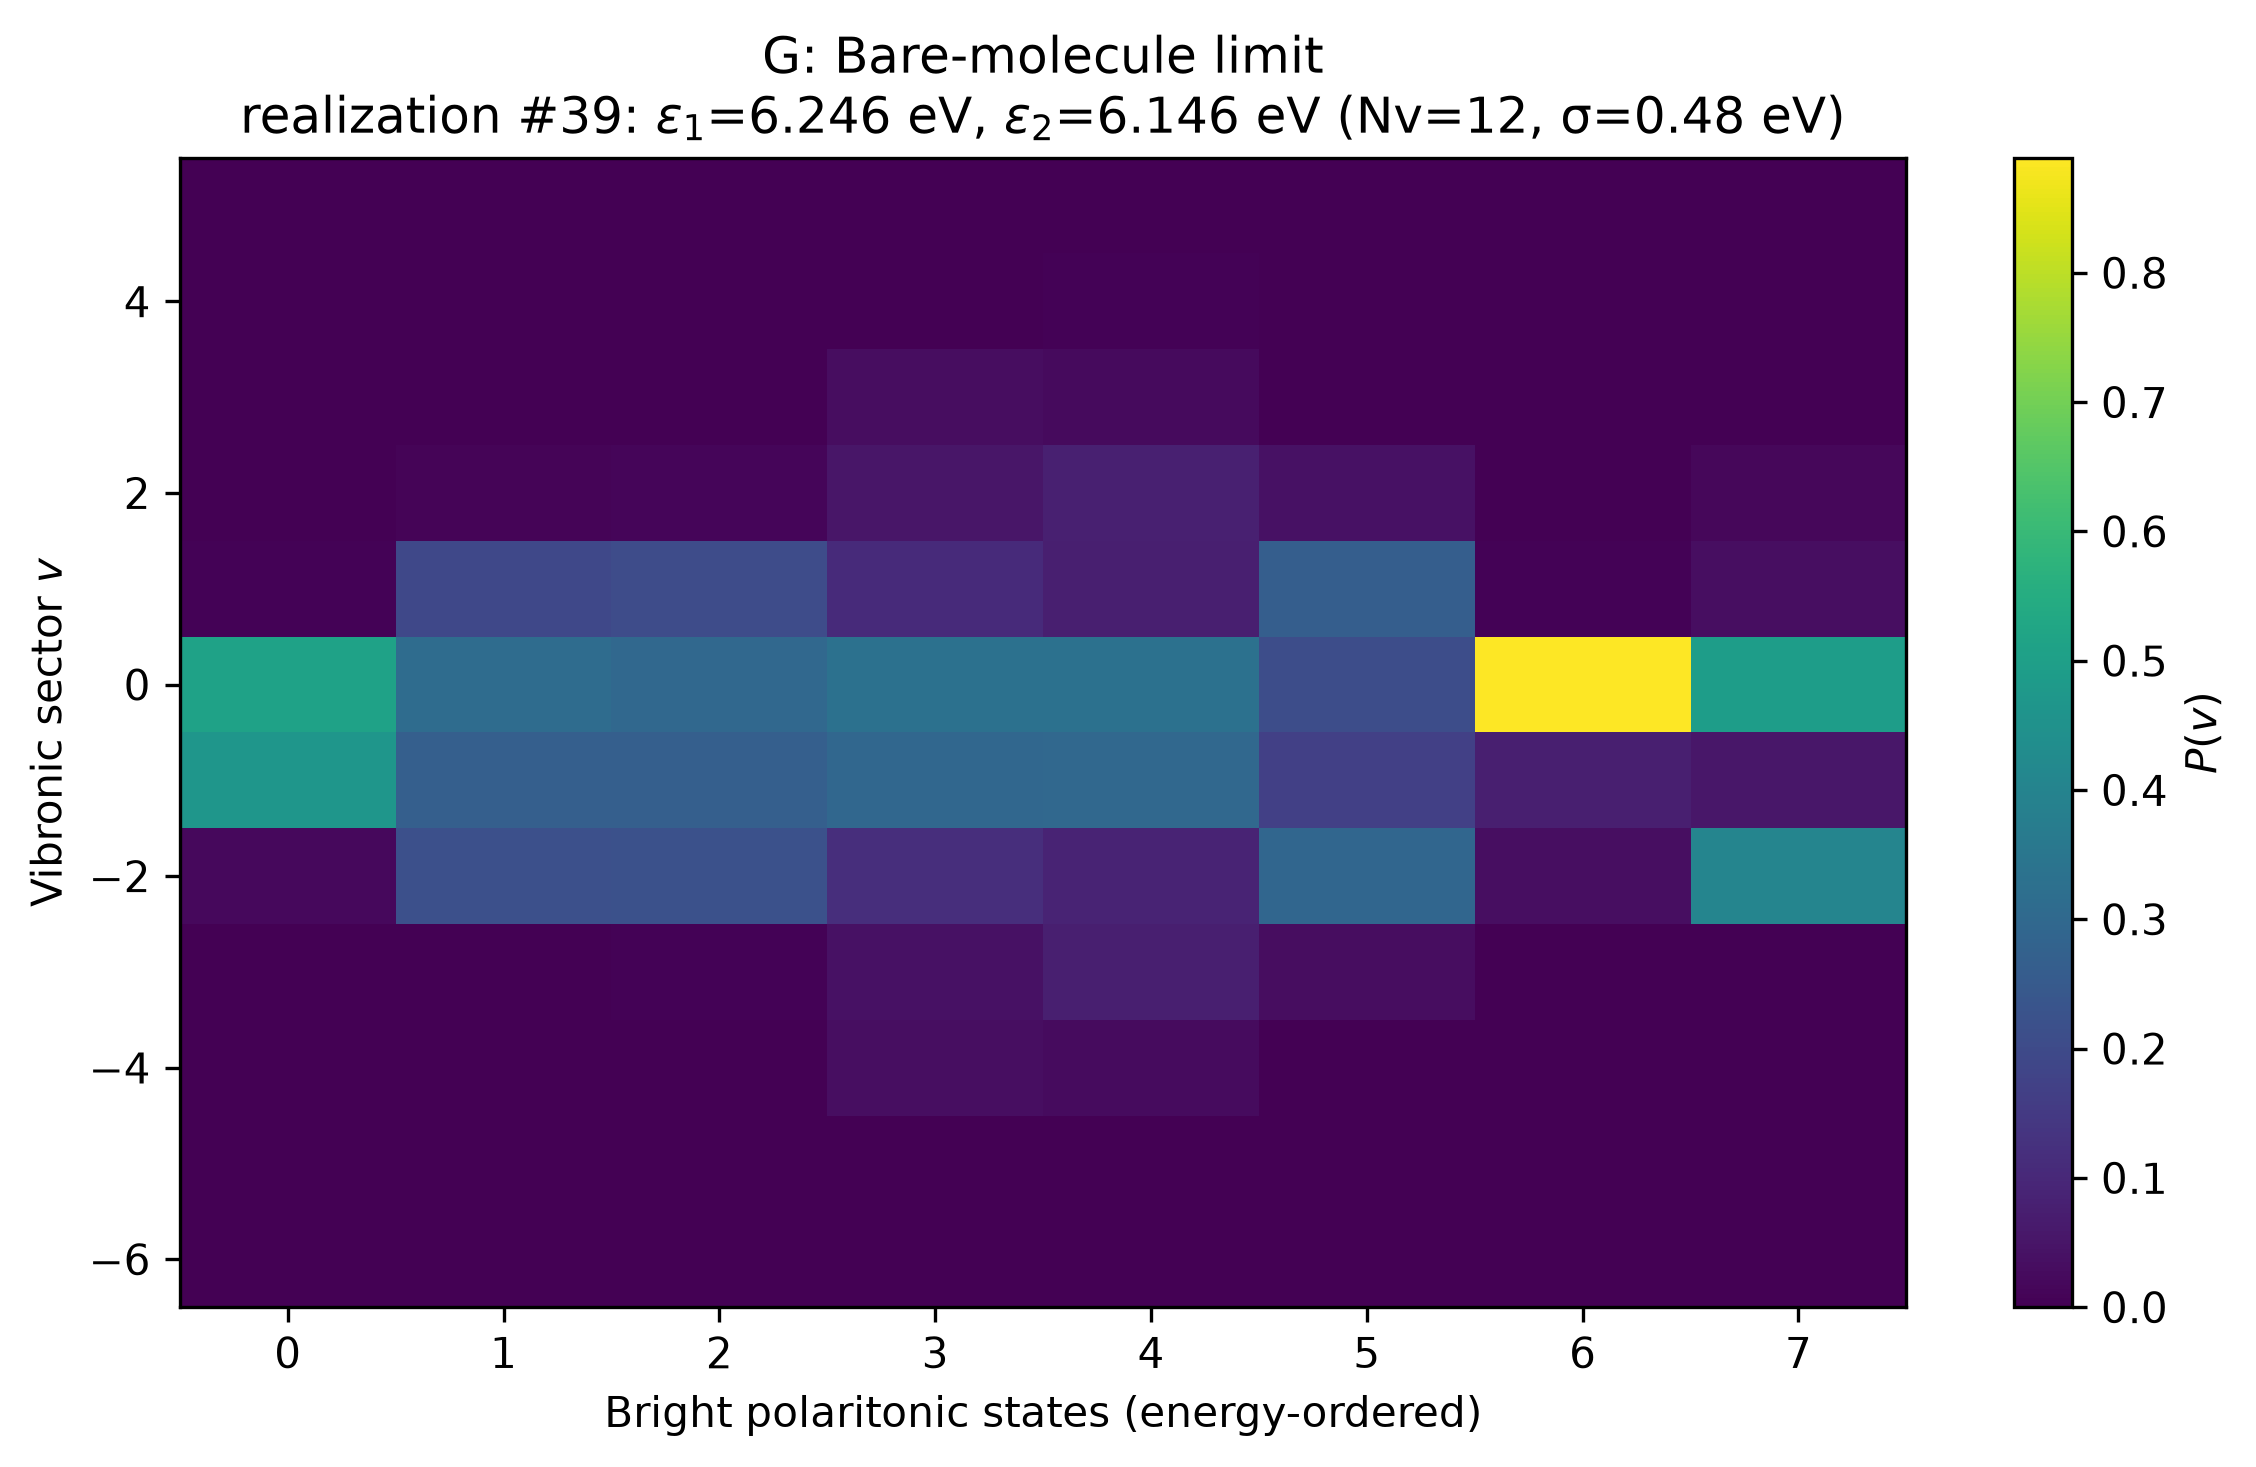
\includegraphics[width=0.44\textwidth]{fig_case_G_heatmap.png}
\caption{\textbf{Case G}, bare-molecule limit,
$(\epsilon_1,\epsilon_2)=(6.246,6.146)$: both molecules pushed far below
resonance together, $s=-3.3g$, $\Delta=0.10$.}
\label{fig:caseG}
\end{figure}
\FloatBarrier

Finally, Case G (Fig.~\ref{fig:caseG}) pushes \emph{both} molecules far below
resonance together:
they remain perfectly matched ($\Delta=0.10$) but sit $s=-3.3g$ - well
outside the polariton band - from the bright line. The absorption collapses
to a single peak at $6.998$~eV, the essentially uncoupled cavity photon, and
the heatmap retains only $8$ bright states confined to $v\in[-4,3]$, one of
which holds $\approx90\%$ of its weight in $v=0$; $\PR_{\max}=4.5$.

Cases B and G are both ``dead'' at nearly the same $\PR_{\max}\approx4$, but
they die by \emph{different} mechanisms - a distinction that is one of the
main results of this work. B dies along the \emph{mismatch} axis: $\Delta\gg g$
decouples the molecules from each other and the excitation localizes on one,
giving a bounded single-molecule cascade. G dies along the \emph{common-mode}
axis: the molecules stay perfectly matched, but $|s|\gg\sqrt N g$ places both
outside the polariton band, so the bright eigenstate reverts to the bare photon
and the cavity-mediated exchange driving the cascade is switched off.

\subsection{Overview: bright states and cascade strength across cases}

\begin{figure}[htbp]
\centering
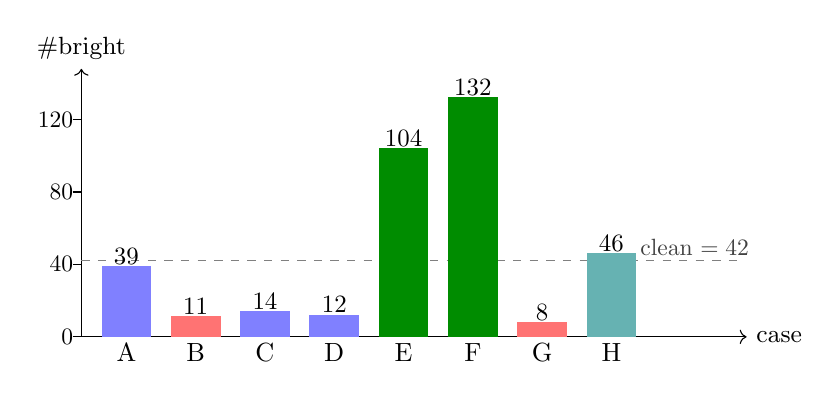
\begin{tikzpicture}[yscale=0.92,xscale=0.88]
  \draw[->] (-0.3,0)--(9.3,0) node[right]{\small case};
  \draw[->] (-0.3,0)--(-0.3,3.7) node[above]{\small \#bright};
  \foreach \y/\l in {0/0,1/40,2/80,3/120}
    {\draw (-0.42,\y)--(-0.3,\y) node[left,scale=0.85]{\l};}
  \draw[dashed,gray] (-0.3,1.05) -- (9.2,1.05);
  \node[gray!50!black,scale=0.85] at (8.55,1.24){clean $=42$};
  \filldraw[blue!50]        (0,0) rectangle (0.7,0.975);
  \filldraw[red!55]         (1,0) rectangle (1.7,0.275);
  \filldraw[blue!50]        (2,0) rectangle (2.7,0.35);
  \filldraw[blue!50]        (3,0) rectangle (3.7,0.30);
  \filldraw[green!55!black] (4,0) rectangle (4.7,2.60);
  \filldraw[green!55!black] (5,0) rectangle (5.7,3.30);
  \filldraw[red!55]         (6,0) rectangle (6.7,0.20);
  \filldraw[teal!60]        (7,0) rectangle (7.7,1.15);
  \foreach \x/\l in {0/A,1/B,2/C,3/D,4/E,5/F,6/G,7/H}
    {\node[scale=0.95] at (\x+0.35,-0.22){\l};}
  \foreach \x/\v/\h in {0/39/0.975,1/11/0.275,2/14/0.35,3/12/0.30,
                        4/104/2.60,5/132/3.30,6/8/0.20,7/46/1.15}
    {\node[scale=0.9] at (\x+0.35,\h+0.14){\v};}
\end{tikzpicture}
\caption{Number of bright polaritonic states per case (intensity above
$10^{-2}$ of the maximum), compared with the clean $N=2$ reference (dashed,
$42$). Green: enhanced (E, F); red: dead (B, G); teal: intermediate (H);
blue: the remaining cases (A, C, D).}
\label{fig:bright}
\end{figure}
\FloatBarrier

Figure~\ref{fig:bright} summarises the bright-state count. Ordering the cases
instead by the cleaner, per-state cascade metric $\PR_{\max}$ gives
\begin{equation*}
  \text{E }(22.4)\ \approx\ \text{F }(21.6)\ \approx\ \text{A }(20.6)
  \ >\ \text{H }(16.2)\ >\ \text{D }(12.5)\ >\ \text{C }(8.5)
  \ >\ \text{G }(4.5)\ \approx\ \text{B }(3.8).
\end{equation*}
This ordering also separates cleanly into three groups rather than forming a
smooth trend: E, F and A cluster at or above the clean value; H, D and C form
a middle band; and G, B sit together at the bottom, an order of magnitude
lower. Neither grouping lines up with the mismatch $\Delta$ alone: Case G's
mismatch ($\Delta=0.10$) is far smaller than Case H's ($\Delta=2.5g$), yet G
is dead and H is only partially degraded. This three-way split is itself a
hint that a single
disorder magnitude does not set the outcome; Sec.~\ref{sec:discussion} makes
precise what does.

%=============================================================================
\section{Discussion}\label{sec:discussion}
%=============================================================================

Every case above can be described through a single candidate mechanism,
\textbf{bright/dark mixing}, adapted from the random-arrowhead-matrix analysis
of Ref.~\cite{Dubail2021}. That analysis was carried out for the disordered
Tavis--Cummings (Holstein-type) model, where each molecule contributes a
single excited level; our JT molecules instead carry a full vibronic cascade,
and extending the arrowhead proof to that richer setting has not been done
here. With that caveat, the qualitative picture is as follows. In the clean,
matched, resonant system the permutation symmetry splits the two-molecule
matter states into a bright symmetric combination
$(\ket{E,A}+\ket{A,E})/\sqrt2$, which carries all the photon coupling and
forms the LP/UP pair split off by $\pm\sqrt N g$, and a dark antisymmetric
combination with zero photon weight and hence zero intensity - this part is
exact, independent of the vibronic richness (Sec.~\ref{sec:cavity}).

Whether this exact, clean-limit coupling is actually what drives the
case-by-case behaviour of Sec.~\ref{sec:results}, rather than merely being
consistent with it, is left open (see Caveats below). The key point from that
case-by-case evidence is that
the outcome is \emph{not} monotonic in the disorder magnitude. Moderate mixing
- the bright polariton pushed \emph{towards} the dense dark manifold, as in
E and F - is a plausible reason why more of the cascade becomes visible than
in the clean system, matching the enhancement Ref.~\cite{Wellnitz2022}
describes for the simpler Holstein-type model. Excessive mixing, or mixing in
the wrong direction, coincides with the cascade being destroyed instead.
Which of the two happens is governed by
proximity to cavity resonance and to the collective coupling scale, not by
$|\delta_1|,|\delta_2|$ alone.

\paragraph{Caveats.} Three limitations should be kept in mind. (i)~Each case is
a \emph{single} extremal draw chosen to illustrate a mechanism; $\PR$ and
\#bright fluctuate strongly between realizations, so quantitative claims would
require averaging over all realizations at fixed $W$. (ii)~\#bright depends on
the brightness threshold. (iii)~The
``bright/dark'' language is borrowed from the $N\to\infty$ arrowhead-matrix
limit of Ref.~\cite{Dubail2021}, itself proved for the disordered
Tavis--Cummings (Holstein-type) model rather than a JT vibronic cascade;
extending that proof to our model, and to the $N=2$ case specifically, remains
to be done. With two molecules there is only one dark combination per
vibronic channel, so ``brightening'' means antisymmetric channels gaining
photon weight, not the filling of a large dark band.

%=============================================================================
\section{Summary and conclusions}\label{sec:summary}
%=============================================================================

\begin{enumerate}\itemsep2pt
  \item \textbf{Reproduced} the single-molecule cavity Jahn--Teller polariton
  spectrum of Ref.~\cite{Nandipati2023} - LP/UP branches, bounded vibronic
  sectors $v\in\{0,-1,-2\}$ - and the two-molecule collective spectrum of
  Ref.~\cite{Pandit2025} together with its $P(v)$ heatmap, recovering the
  unbounded cascade with $\PR$ up to $\approx20$ over $42$ bright states.
  \item \textbf{Introduced static Gaussian energy disorder} into the $N=2$
  cavity-JT model, following the disordered Holstein--Tavis--Cummings
  \cite{Wellnitz2022} and random-arrowhead \cite{Dubail2021} frameworks:
  $\epsilon_i\sim\mathcal N(\epsilon,W^2)$, with the spectrum built from the
  photon weight of each eigenstate of the $(n_{\mathrm{ex}}=1,j=-1)$ block,
  Lorentzian broadened and averaged over realizations.
  \item \textbf{Implemented and analysed} the disorder layer: symmetry
  filtering from $746\,496$ to $6\,900$ basis states, a representative-%
  realization analysis recovering the individual draws behind the average,
  eight physically selected cases and a $P(v)$
  heatmap for each, validated by regression tests and by the near-zero-disorder
  control (Case A).
  \item \textbf{Key result.} Whether disorder destroys the collective vibronic
  cascade depends on whether it pushes the bright polariton \emph{closer to}
  the dense manifold of otherwise-dark states or \emph{pulls it away} -
  governed by proximity to cavity resonance and to the collective coupling
  scale, not by the disorder magnitude alone. In the favourable direction
  disorder \emph{enhances} the observable cascade (Cases E and F: $104$ and
  $132$ bright states versus $42$ for the clean system, at undiminished
  $\PR$); in the unfavourable ones it destroys it by two distinct routes,
  localization on a single molecule (Case B) and decoupling from the cavity
  (Case G).
\end{enumerate}

Natural continuations are to map $\PR$ over the mismatch and common-mode shift
more broadly at
several disorder widths, to separate convergence in the vibrational cutoff
$N_v$ from the disorder effect, and to extend the analysis to $N>2$, where the
dark manifold becomes a genuine band and the arrowhead predictions apply
quantitatively.

%=============================================================================
\small
\begin{thebibliography}{99}
\setlength{\itemsep}{0pt}\setlength{\parskip}{0pt}
%=============================================================================

\bibitem{Nandipati2023}
K.~R.~Nandipati and O.~Vendrell,
\textit{Cavity Jahn-Teller polaritons in molecules},
Phys.\ Rev.\ A \textbf{107}, L061101 (2023).

\bibitem{Pandit2025}
S.~K.~Pandit, A.~Pandey, A.~Shankar and K.~R.~Nandipati,
\textit{Collective Vibronic Cascade in Cavity-Coupled Jahn-Teller Active
Molecules}, arXiv:2511.07880 [quant-ph] (2025).

\bibitem{Dubail2021}
C.~Dubail, T.~Botzung, J.~Schachenmayer, G.~Pupillo and D.~Hagenm\"uller,
\textit{Large random arrowhead matrices: multifractality, semi-localization,
and protected transport in disordered quantum spins coupled to a cavity},
arXiv:2105.08444 (2021); Phys.\ Rev.\ A \textbf{105}, 023714 (2022).

\bibitem{Wellnitz2022}
D.~Wellnitz, G.~Pupillo and J.~Schachenmayer,
\textit{Disorder enhanced vibrational entanglement and dynamics in
polaritonic chemistry},
Commun.\ Phys.\ \textbf{5}, 120 (2022).

\bibitem{JahnTeller1937}
H.~A.~Jahn and E.~Teller,
\textit{Stability of polyatomic molecules in degenerate electronic states.
I. Orbital degeneracy},
Proc.\ R.\ Soc.\ Lond.\ A \textbf{161}, 220 (1937).

\bibitem{LonguetHiggins1958}
H.~C.~Longuet-Higgins, U.~\"Opik, M.~H.~L.~Pryce and R.~A.~Sack,
\textit{Studies of the Jahn-Teller effect. II. The dynamical problem},
Proc.\ R.\ Soc.\ Lond.\ A \textbf{244}, 1 (1958).

\bibitem{Bersuker2006}
I.~B.~Bersuker,
\textit{The Jahn-Teller Effect} (Cambridge University Press, Cambridge, 2006).

\bibitem{Koppel1984}
H.~K\"oppel, W.~Domcke and L.~S.~Cederbaum,
\textit{Multimode molecular dynamics beyond the Born-Oppenheimer
approximation},
Adv.\ Chem.\ Phys.\ \textbf{57}, 59 (1984).

\bibitem{Whetten1986}
R.~L.~Whetten, K.~S.~Haber and E.~R.~Grant,
\textit{The dynamic Jahn-Teller effect in sym-triazine: Nonadiabatic wave
functions and hindered fluxionality},
J.\ Chem.\ Phys.\ \textbf{84}, 1270 (1986).

\bibitem{Harris1989}
D.~C.~Harris and M.~D.~Bertolucci,
\textit{Symmetry and Spectroscopy: An Introduction to Vibrational and
Electronic Spectroscopy} (Dover, New York, 1989).

\bibitem{Ebbesen2016}
T.~W.~Ebbesen,
\textit{Hybrid light-matter states in a molecular and material science
perspective},
Acc.\ Chem.\ Res.\ \textbf{49}, 2403 (2016).

\bibitem{Feist2018}
J.~Feist, J.~Galego and F.~J.~Garcia-Vidal,
\textit{Polaritonic chemistry with organic molecules},
ACS Photonics \textbf{5}, 205 (2018).

\bibitem{Herrera2016}
F.~Herrera and F.~C.~Spano,
\textit{Cavity-controlled chemistry in molecular ensembles},
Phys.\ Rev.\ Lett.\ \textbf{116}, 238301 (2016).

\bibitem{Barnett2012}
S.~M.~Barnett, R.~P.~Cameron and A.~M.~Yao,
\textit{Duplex symmetry and its relation to the conservation of optical
helicity},
Phys.\ Rev.\ A \textbf{86}, 013845 (2012).

\bibitem{Crisp1991}
M.~D.~Crisp,
\textit{Jaynes-Cummings model without the rotating-wave approximation},
Phys.\ Rev.\ A \textbf{43}, 2430 (1991).

\bibitem{Nandipati2021}
K.~R.~Nandipati and O.~Vendrell,
\textit{Dynamical Jahn-Teller effects on the generation of electronic ring
currents by circularly polarized light},
Phys.\ Rev.\ Research \textbf{3}, L042003 (2021).

\bibitem{Vendrell2018}
O.~Vendrell,
\textit{Coherent dynamics in cavity femtochemistry: Application of the
multi-configuration time-dependent Hartree method},
Chem.\ Phys.\ \textbf{509}, 55 (2018).

\bibitem{Harris2020}
C.~R.~Harris \emph{et al.},
\textit{Array programming with NumPy},
Nature \textbf{585}, 357 (2020).

\bibitem{Virtanen2020}
P.~Virtanen \emph{et al.},
\textit{SciPy 1.0: fundamental algorithms for scientific computing in
Python},
Nat.\ Methods \textbf{17}, 261 (2020).

\bibitem{Hunter2007}
J.~D.~Hunter,
\textit{Matplotlib: A 2D graphics environment},
Comput.\ Sci.\ Eng.\ \textbf{9}, 90 (2007).

\end{thebibliography}

\end{document}
